\documentclass[12pt]{article}

\usepackage[a4paper, left=1.2in, right=1.2in]{geometry}
\usepackage{setspace}
\usepackage[utf8]{inputenc}
\usepackage[italian]{babel}
\usepackage[OT1]{fontenc}
\usepackage{graphicx}
\usepackage{subcaption}
\usepackage{float}
\usepackage{fancyhdr}
\usepackage{xcolor}
\usepackage{mathtools}
\usepackage{amsmath}
\usepackage{amssymb}
\usepackage{tikz}
\usepackage{imakeidx}
\usepackage{textcomp}
\usepackage{pifont}
\usepackage{polynom}
\usepackage{algorithm}
\usepackage{algpseudocode}
\usepackage{mathtools}
\usepackage[colorlinks=true,linkcolor=black,anchorcolor=black,citecolor=black,filecolor=black,menucolor=black,runcolor=black,urlcolor=black]{hyperref}
\usepackage{cancel}
\usepackage{pgfplots}
\usepackage{caption}
\usepackage{tabularx}
\usepackage{comment}
\usepackage{float}
\usepackage{bm}



\onehalfspacing

\begin{document}
\bibliographystyle{plain}
    \pagestyle{fancy}
    \everymath{\displaystyle}
    \sffamily
    \begin{figure}
        \centering
        
\includegraphics[scale=0.1]{images/uniba-logo.png}
        \caption*{Università degli Studi di Bari Aldo Moro}
    \end{figure}
    \begin{figure}
        \centering
        
\includegraphics[scale=0.1]{images/swap.png}
        \caption*{Gruppo di ricerca Semantic Web Access and Personalization}
    \end{figure}
    

    \title{
        Tesi in Metodi per il Ritrovamento dell'Informazione\\   
    \textbf{Sustainability of RecSys}}
    \date{Tesi triennale in Informatica\\Anno accademico 2023/2024}
    \maketitle

\begin{itemize}
    \item \textbf{Relatore}: Prof. Pasquale Lops
    \item \textbf{Relatore}: Prof. Cataldo Musto
    \item \textbf{Laureando}: Emanuele Fontana
\end{itemize}
\newpage
    \tableofcontents
    \newpage
    \section*{ABSTRACT}
\addcontentsline{toc}{section}{ABSTRACT}
Lo scopo di questa tesi è quello di analizzare la sostenibilità ambientale dei sistemi di raccomandazione, in particolare di quelli basati su algoritmi di apprendimento automatico.Si vuole indagare su quello che è il trade-off tra le performance dei modelli di raccomandazione a stato dell'arte e il loro impatto ambientale e vedere se sia possibile ridurre quest'ultimo senza compromettere in modo significativo le performance.Per fare ciò si è scelto di addestrare alcuni modelli di raccomandazione a stato dell'arte su dataset di dimensioni diverse e cercare di capire il trade-off tra performance e impatto ambientale di ciascuno di essi. Successivamente si è cercato di ridurre l'impatto ambientale di questi modelli lavorando sul criterio di early stopping, cercando di capire se sia possibile utilizzare un criterio di early stopping basato anche sulle emissioni dei modelli. Anche questi esperimenti sono stati condotti su dataset di dimensioni diverse e sui diversi modelli di raccomandazione a stato dell'arte per valutare il trade-off tra performance e impatto ambientale. Successivamente si sono confrontati i risultati ottenuti con quelli precedenti.I risultati ottenuti mostrano che, in generale, è possibile ridurre l'impatto ambientale dei modelli di raccomandazione senza compromettere in modo significativo le performance dei modelli stessi.
\setcounter{section}{0}
\renewcommand{\thesection}{\arabic{section}}
    \newpage
    \input{pages/sostenibilità.tex}
    \newpage
    \section{Recommender Systems}

\subsection{Introduzione}

Un sistema di raccomandazione (Recommender System) \cite{RecommenderOverview} è un sistema software progettato per suggerire all'utente elementi di interesse, come ad esempio prodotti, servizi, informazioni o contenuti multimediali, in base alle preferenze e ai comportamenti passati dell'utente. I sistemi di raccomandazione sono ampiamente utilizzati in diversi contesti, come ad esempio il commercio elettronico, i social network, i servizi di streaming multimediale e le piattaforme di ricerca e informazione. I sistemi di raccomandazione sono utili per migliorare l'esperienza dell'utente, aumentare la soddisfazione e la fidelizzazione del cliente, e favorire la scoperta di nuovi contenuti e opportunità.
Questi sistemi sono basati su algoritmi di apprendimento automatico e intelligenza artificiale, che analizzano i dati relativi alle preferenze e ai comportamenti degli utenti, e generano raccomandazioni personalizzate in base a tali informazioni.\\

\begin{figure}[h!]
    \centering
    \begin{minipage}{0.2\textwidth}
        \centering
        
\includegraphics[width=\textwidth]{images/netflix.png}
    \end{minipage}\hfill
    \begin{minipage}{0.2\textwidth}
        \centering
        
\includegraphics[width=\textwidth]{images/amazon.png}
    \end{minipage}\hfill
    \begin{minipage}{0.2\textwidth}
        \centering
        
\includegraphics[width=\textwidth]{images/spotify.png}
    \end{minipage}\hfill
    \begin{minipage}{0.2\textwidth}
        \centering
        
\includegraphics[width=\textwidth]{images/tiktok.png}
    \end{minipage}
    \caption{Alcuni famose piattaforme che utilizzano sistemi di raccomandazione}
\end{figure}


\noindent I sistemi di raccomandazione possono essere di diversi tipi, a seconda della tecnica utilizzata per generare le raccomandazioni.
\begin{itemize}
    \item \textbf{Collaborative filtering} \cite{CFRS}
    \item \textbf{Content-based} \cite{Lops2011}
    \item \textbf{Knowledge-based} \cite{KnowledgeBased}
    \item \textbf{Approci ibridi}: combinano le tecniche precedenti
\end{itemize}



\begin{table}[H]
    \centering
    \footnotesize
    \setlength\tabcolsep{0pt}
    \begin{tabularx}{\textwidth}{|X|X|}
        \hline
        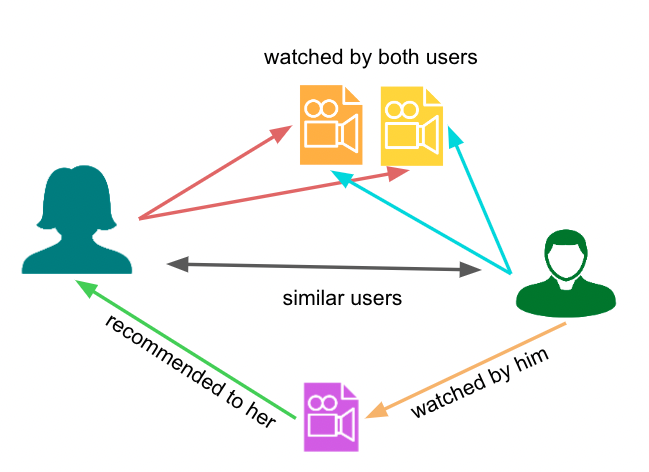
\includegraphics[width=\linewidth, trim=0 0 0 0]{images/cfRecSys.png} &
        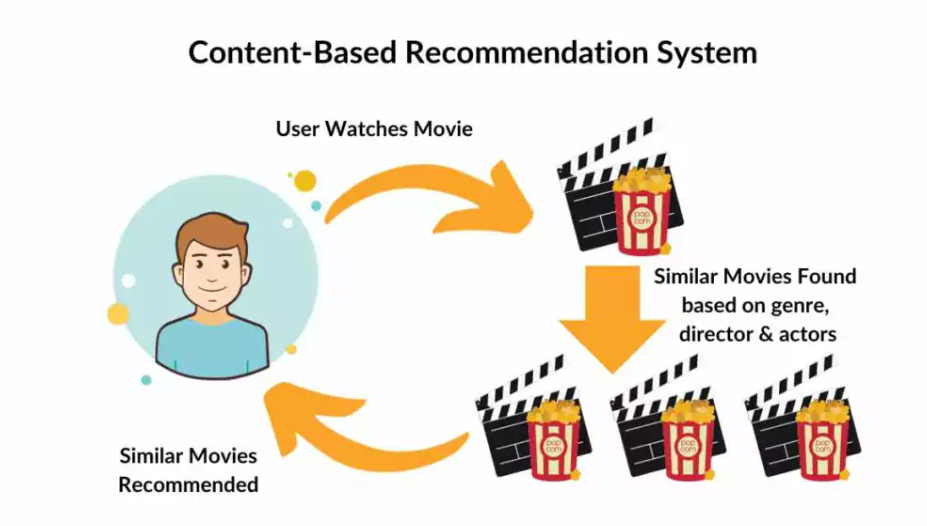
\includegraphics[width=\linewidth, trim=0 0 0 0]{images/contentbased.png} \\
        \hline
        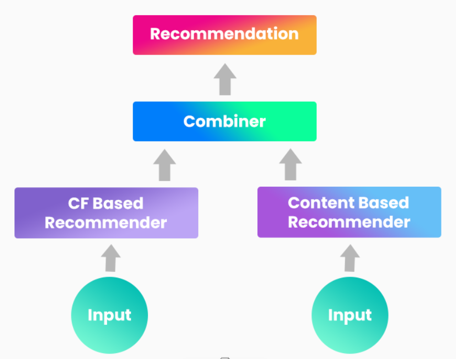
\includegraphics[width=\linewidth, trim=0 0 0 0]{images/hybridRecSys.png} &
        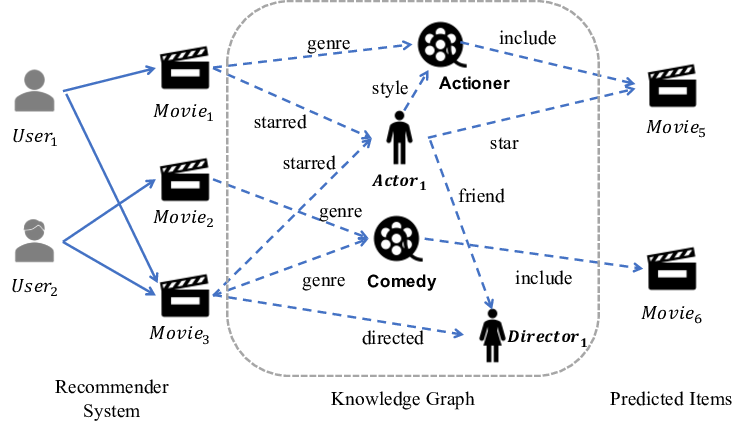
\includegraphics[width=\linewidth, trim=0 0 0 0]{images/knowledge.png} \\
        \hline
    \end{tabularx}
    \caption{Tipi di Recommender Systems}
\end{table}


\noindent Per valutare le prestazioni di un sistema di raccomandazione si possono utilizzare diverse metriche che è possibile riassumere nelle seguenti categorie:
\begin{itemize}
    \item \textbf{Accuracy metrics}: queste metriche valutano la precisione e l'accuratezza delle raccomandazioni generate dal sistema. Alcune delle metriche più comuni sono l'RMSE (Root Mean Squared Error) e il MAE (Mean Absolute Error).
    \item \textbf{Ranking metrics}: queste metriche valutano la qualità dell'ordinamento delle raccomandazioni generate dal sistema. Alcune delle metriche più comuni sono il coefficiente di correlazione di Kendall Tau, il coefficiente di correlazione di Spearman, l'NDCG (Normalized Discounted Cumulative Gain).
    \item \textbf{Diversity metrics}: queste metriche valutano la diversità delle raccomandazioni generate dal sistema. Alcune delle metriche più comuni sono la diversità delle raccomandazioni e la novità delle raccomandazioni.
    \item \textbf{Coverage metrics}: queste metriche valutano la copertura degli elementi raccomandati dal sistema.
    
    \item \textbf{Classification metrics}: queste metriche valutano la capacità del sistema di classificare correttamente gli elementi in base alle preferenze dell'utente. Alcune delle metriche più comuni sono l'accuracy, la precision, il recall e l'F1-score.
\end{itemize}

\noindent Alcuni tipici problemi che si possono incontrare nella progettazione e nell'implementazione di un sistema di raccomandazione sono:
\begin{itemize}
    \item \textbf{Cold start problem} \cite{ColdStart}: il problema del cold start si verifica quando un nuovo utente o un nuovo elemento si registra nel sistema e non ci sono dati sufficienti per generare raccomandazioni personalizzate.
    \item \textbf{Data sparsity problem} \cite{DataSparsity}: nella maggior parte delle reali applicazioni il numero di item è molto maggiore del numero di item valutati da ciascun utente. Questo porta a una matrice di valutazioni molto sparsa, che rende difficile la generazione di raccomandazioni accurate
    \item \textbf{Vulnerabilità agli attacchi} \cite{Attacchi} : i sistemi di raccomandazione possono essere vulnerabili a diversi tipi di attacchi, come ad esempio le recensioni fake (tipico problema degli e-commerce)
\end{itemize}

\subsection{Collaborative Filtering}
I sistemi di raccomandazione collaborative filtering generano raccomandazioni/filtrano i contenuti basandosi sull' "opinione" di altri utenti.\\ Con il termine utente ci si riferisce a qualsiasi individuo che inserisca delle valutazioni per gli item presenti nel sistema. \\ Gli item sono gli oggetti che vengono raccomandati agli utenti (es. film, libri, prodotti, etc.).\\
L'idea alla base del collaborative filtering è creare una matrice di valutazioni utente-item, in cui ogni cella della matrice rappresenta la valutazione di un utente per un item.\\ Le valutazioni sono in genere numeriche, e possono essere espresse in termini di rating (es. da 1 a 5 stelle) o di preferenze (es. like/dislike).\\
Esistono principalmente due tipi di collaborative filtering:
\begin{itemize}
    \item \textbf{User-based collaborative filtering}: in questo approccio, le raccomandazioni vengono generate confrontando le preferenze dell'utente con quelle degli altri utenti. In particolare, si calcola la similarità tra l'utente target e gli altri utenti, e si generano raccomandazioni basate sulle preferenze degli utenti più simili all'utente target. Due utenti sono ritenuti simili se hanno uno stile di valutazione simile per gli item (cioè valutano gli stessi item in modo simile)
    \item \textbf{Item-based collaborative filtering}: in questo approccio, le raccomandazioni vengono generate confrontando le preferenze degli utenti per gli item. In particolare, si calcola la similarità tra gli item, e si generano raccomandazioni basate sugli item più simili a quelli valutati positivamente dall'utente target. Due item sono ritenuti simili se vengono valutati in modo simile dagli stessi utenti.
\end{itemize}
I principali vantaggi del collaborative filtering sono la sua semplicità e la sua capacità di generare raccomandazioni personalizzate senza la necessità di dover conoscere le caratteristiche degli item (es. la durata di un film, il genere di un libro, etc.). Tuttavia, il collaborative filtering può soffrire di problemi come il cold start (per un nuovo utente e per un nuovo item), la vulnerabilità agli attacchi come le recensioni fake e la scarsa spiegaibilità delle raccomandazioni generate.\\

%crea un esempio di matrice utente-item
\begin{table}[H]
    \centering
    \begin{tabular}{|c|c|c|c|c|}
        \hline
        & Item 1 & Item 2 & Item 3 & Item 4 \\
        \hline
        User 1 & 5 & 4 & 0 & 0 \\ \hline
        User 2 & 0 & 0 & 3 & 4 \\ \hline
        User 3 & 0 & 0 & 0 & 0 \\ \hline
        User 4 & 0 & 0 & 0 & 0 \\
        \hline
    \end{tabular}
    \caption{Esempio di matrice utente-item}
\end{table}


\subsection{Content-based}
I sistemi di raccomandazione content-based generano raccomandazioni basate sul contenuto degli elementi e sulle preferenze dell'utente. Questi sistemi analizzano le caratteristiche degli elementi e le preferenze dell'utente, e generano raccomandazioni in base alla somiglianza tra gli elementi e le preferenze dell'utente. Per preferenze dell'utente si intendono le caratteristiche degli elementi che l'utente ha valutato in passato.
Un sistema di raccomandazione content-based è composto da tre componenti principali:
\begin{itemize}
    \item \textbf{Profile learner}: Questa componente colleziona i dati relativi alle preferenze dell'utente e cerca di generalizzarle per creare un profilo dell'utente. Spesso questa generalizzazione avviene mediante tecniche di apprendimento automatico.
    \item \textbf{Content analyzer}: Questa componente ha come scopo quello di estrarre le caratteristiche degli item. Quando le descrizioni non sono strutturate (es. testo) è necessaria una fase di pre-processing per estrarre le caratteristiche rilevanti.
    \item \textbf{Filtering Component}: Questa componente ha come scopo quello di generare raccomandazioni personalizzate in base al profilo dell'utente e alle caratteristiche degli item. In particolare, si calcola la somiglianza tra il profilo dell'utente e le caratteristiche degli item, e si generano raccomandazioni basate su questa somiglianza.
\end{itemize}
I principali vantaggi sono l'indipendenza dal comportamento degli altri utenti e la capacità di generare raccomandazioni personalizzate anche per nuovi item. Inoltre c'è una maggiore spiegabilità delle raccomandazioni generate. Tuttavia, i sistemi di raccomandazione content-based possono soffrire di problemi come la scarsa diversità delle raccomandazioni e la difficoltà di estrarre le caratteristiche rilevanti degli item. Rimane comunque il problema di cold-start per un nuovo utente.
\subsection{Knowledge-based}
I sistemi di raccomandazione knowledge-based generano raccomandazioni basandosi su conoscenza semantica, rappresentata mediante i knowledge-graph. I knowledge-graph sono grafi in cui i nodi rappresentano concetti e le relazioni tra i concetti, e gli archi rappresentano le relazioni tra i concetti. I sistemi di raccomandazione knowledge-based utilizzano i knowledge-graph per rappresentare le caratteristiche degli item e le preferenze dell'utente, e generare raccomandazioni basate su questa rappresentazione. In particolare, si utilizzano tecniche di reasoning per inferire nuove conoscenze a partire dalle conoscenze esistenti, e generare raccomandazioni basate su queste nuove conoscenze. I principali vantaggi dei sistemi di raccomandazione knowledge-based l'assenza del problema di cold-start. Tuttavia, i sistemi di raccomandazione knowledge-based possono soffrire di problemi come la scarsa spiegabilità delle raccomandazioni generate e la difficoltà di rappresentare la conoscenza semantica in modo accurato e completo. Inoltre, i sistemi di raccomandazione knowledge-based possono richiedere una quantità significativa di risorse computazionali per generare raccomandazioni accurate e rilevanti.\\

\subsection{Modelli di raccomandazione a stato dell'arte}
Negli ultimi anni, sono stati proposti diversi modelli di raccomandazione basati su diverse tecniche, che hanno ottenuto risultati molto promettenti in termini di accuratezza e prestazioni. Questi modelli sono chiamati a stato dell'arte (\textbf{SOTA:}state-of-the-art) per l'implementazione di sistemi di raccomandazione. Alcuni esempi di modelli di raccomandazione a stato dell'arte sono:
\begin{itemize}
    \item \textbf{ItemKNN} \cite{ItemKNN}: ItemKNN è un modello di raccomandazione basato su collaborative filtering item-based. In particolare, ItemKNN calcola la similarità tra gli item e genera raccomandazioni basate sugli item più simili a quelli valutati positivamente dall'utente target.
    \item \textbf{BPR} \cite{BPR}: BPR (Bayesian Personalized Ranking) è un modello di raccomandazione basato su collaborative filtering user-based. In particolare, BPR calcola la similarità tra gli utenti e genera raccomandazioni basate sugli utenti più simili all'utente target.
    \item \textbf{CFKG} \cite{CFKG}: CFKG è un modello di raccomandazione basato su collaborative filtering e knowledge-based. In particolare, CFKG utilizza i knowledge-graph per rappresentare le caratteristiche degli item e le preferenze dell'utente, e genera raccomandazioni basate su questa rappresentazione.
    \item \textbf{CKE} \cite{CKE}: CKE (Collaborative Knowledge Embedding) è un modello di raccomandazione basato su collaborative filtering e knowledge-based. In particolare, CKE utilizza tecniche di embedding per rappresentare le caratteristiche degli item e le preferenze dell'utente, e genera raccomandazioni basate su questa rappresentazione.
    \item \textbf{DMF} \cite{DMF}: DMF (Deep Matrix Factorization) è un modello di raccomandazione basato su deep learning. In particolare, DMF utilizza tecniche di deep learning per apprendere le rappresentazioni latenti degli item e degli utenti, e genera raccomandazioni basate su queste rappresentazioni.
    \item \textbf{KGCN} \cite{KGCN}: KGCN (Knowledge Graph Convolutional Networks) è un modello di raccomandazione basato su deep learning e knowledge-based. In particolare, KGCN utilizza tecniche di deep learning e convolutional neural networks per apprendere le rappresentazioni degli item e degli utenti a partire dai knowledge-graph, e genera raccomandazioni basate su queste rappresentazioni.
    \item \textbf{KGNNLS} \cite{KGNNLS}: KGNNLS (Knowledge Graph Neural Network with Latent Space) è un modello di raccomandazione basato su deep learning e knowledge-based. In particolare, KGNNLS utilizza tecniche di deep learning e neural networks per apprendere le rappresentazioni degli item e degli utenti a partire dai knowledge-graph, e genera raccomandazioni basate su queste rappresentazioni.
    \item \textbf{LINE} \cite{LINE}: LINE (Large-scale Information Network Embedding) è un modello di raccomandazione basato su deep learning e knowledge-based. In particolare, LINE utilizza tecniche di deep learning e neural networks per apprendere le rappresentazioni degli item e degli utenti a partire dai knowledge-graph, e genera raccomandazioni basate su queste rappresentazioni.
    \item \textbf{MultiDAE} \cite{MultiDAE}: MultiDAE è un modello di raccomandazione basato su deep learning. In particolare, MultiDAE utilizza tecniche di deep learning e variational autoencoders per apprendere le rappresentazioni latenti degli item e degli utenti, e genera raccomandazioni basate su queste rappresentazioni.
    \item \textbf{LightGCN} \cite{LightGCN}: LightGCN è un modello di raccomandazione basato su deep learning. In particolare, LightGCN utilizza tecniche di deep learning e graph convolutional networks per apprendere le rappresentazioni latenti degli item e degli utenti, e genera raccomandazioni basate su queste rappresentazioni.
    \item \textbf{NGCF} \cite{NGCF}: NGCF (Neural Graph Collaborative Filtering) è un modello di raccomandazione basato su deep learning. In particolare, NGCF utilizza tecniche di deep learning e graph convolutional networks per apprendere le rappresentazioni latenti degli item e degli utenti, e genera raccomandazioni basate su queste rappresentazioni.
    \item \textbf{DGCF} \cite{DGCF}: DGCF (Dual Graph Collaborative Filtering) è un modello di raccomandazione basato su deep learning. In particolare, DGCF utilizza tecniche di deep learning e graph convolutional networks per apprendere le rappresentazioni latenti degli item e degli utenti, e genera raccomandazioni basate su queste rappresentazioni.
\end{itemize}


\noindent Ovviamente ci sono tanti altri modelli di raccomandazione a stato dell'arte, ma questi sono solo alcuni esempi.\\
I progettisti di RecSys spesso prendono spunto da questi modelli per creare nuovi modelli che possano adattarsi meglio alle esigenze specifiche del problema che si vuole risolvere.\\



\subsection{Recommender Systems e Sustainability}

I sistemi di raccomandazione, così come tutti gli altri modelli di AI, possono essere utilizzati per promuovere la sostenibilità in tutti i suoi punti, ad esempio cercando di adempiere agli obiettivi dell'Agenda 2030 \cite{RecommenderSustainability}.

\noindent In ambito \textit{energia pulita e riduzione delle emissioni} viene suggerito come i sistemi di raccomandazione possano essere utilizzati per promuovere l'adozione di comportamenti sostenibili, ad esempio suggerendo all'utente di utilizzare mezzi di trasporto pubblici o condivisi, di ridurre il consumo di energia elettrica o di acquistare prodotti sostenibili. Inoltre, i sistemi di raccomandazione possono essere utilizzati per promuovere l'adozione di energie rinnovabili e la riduzione delle emissioni di gas serra. In questo caso si parla dunque di sistemi di raccomandazione i quali cercano di promuovere comportamenti sostenibili, ma a loro vola per essere addestrati richiedono grandi quantità di dati e di risorse computazionali, che possono avere un impatto negativo sull'ambiente.

\noindent Una soluzione dunque può essere quella di addestrare i modelli di raccomandazione in modo sostenibile, senza però perdere di performance.



    \newpage
    \section{Metodologia}

\subsection{RQs e obiettivi del lavoro}

Le \textbf{RQs} (Research Questions) sono le domande di ricerca che si vogliono risolvere con il lavoro. Queste sono state definite in fase di progettazione del lavoro e sono state utilizzate per guidare lo sviluppo del progetto. Le RQs sono le seguenti:
\begin{itemize}
    \item \textbf{RQ1}: Qual è il trade-off tra emissioni e performance dei modelli di raccomandazione a stato dell'arte?
    \item \textbf{RQ2}: E' possibile usare un criterio di early-stopping basato sulle emissioni per migliorare il trade-off tra emissioni e performance dei modelli di raccomandazione a stato dell'arte?
    \item \textbf{RQ3}: Quali parametri di early-stopping basati sulle emissioni possono essere utilizzati per migliorare il trade-off tra emissioni e performance dei modelli di raccomandazione a stato dell'arte?
\end{itemize}

\noindent Con la prima RQ si vuole dunque analizzare il trade-off tra emissioni e performance dei modelli di raccomandazione a stato dell'arte. Per rispondere a questa domanda si è deciso di addestrare diversi modelli di raccomandazione a stato dell'arte e di analizzare le emissioni e le performance di ognuno di essi. Con la seconda RQ si vuole invece analizzare se lavorare con un criterio di early-stopping basato anche sulle emissioni migliora il trade-off tra emissioni e performance rispetto ad un criterio di early-stopping basato sulle sole performance. Per rispondere a questa domanda si è prima di tutto studiato il criterio di early-stopping classico e capire come esso funziona, si è studiato il miglioramento delle performance di epoca in epoca e si è analizzato il trade-off tra emissioni e performance. Successivamente si è implementato un criterio di early-stopping basato anche sulle emissioni e si è analizzato il trade-off tra emissioni e performance di questo criterio. Infine con la terza RQ si vuole analizzare quali criteri di early-stopping basati sulle emissioni possono essere utilizzati per migliorare il trade-off tra emissioni e performance dei modelli di raccomandazione a stato dell'arte. Per rispondere a questa domanda si è deciso di implementare diversi criteri di early-stopping basati sulle emissioni e di analizzare il trade-off tra emissioni e performance di ognuno di essi fissando il dataset utilizzato.

\subsection{Addestamento dei modelli}

Per quanto riguarda l'addestamento dei modelli, si è deciso di addestrare i modelli di raccomandazione a stato dell'arte utilizzando diversi dataset. I modelli di raccomandazione a stato dell'arte addestrati sono i seguenti: ItemKNN, BPR, CFKG, CKE, DMF, KGCN, KGNNLS, LINE, MultiDAE, LightGCN, NFCF, DGCF i quali sono tutti presenti in un framework di raccomandazione a stato dell'arte chiamato \textbf{RecBole} \cite{recbole}.\\
Possiamo dividere questi modelli in due gruppi:
\begin{itemize}
    \item \textbf{Modelli di raccomandazione generali CF}: BPR,CFKG, DMF, KGNNLS, LINE, MultiDAE, LightGCN, ItemKNN. Questi modelli sfruttano le sole valutazioni degli utenti per fare raccomandazioni.
    \item \textbf{Modelli di raccomandazione basati su conoscenza}: CKE, KGCN, NFCF, DGCF. Questi modelli sfruttano sia le valutazioni degli utenti che delle conoscenze aggiuntive (knowledge graph) per fare raccomandazioni.
\end{itemize}
\noindent Dunque questi modelli sono stati scelti in quanto rappresentati delle loro categorie (Collaborative Filtering puro, Deep Learning, Graph Neural Network, Knowledge Graph).\\ 
Sono stati usati dei dataset di dimensioni diverse per poter analizzare il comportamento dei modelli in base alla dimensione del dataset. Durante questo lavoro i dataset utilizzati sono i seguenti: \footnote{https://grouplens.org}{\textbf{Movielens-1m}}, \footnote{https://grouplens.org}{\textbf{Movielens-10m}}, \footnote{https://jmcauley.ucsd.edu/data/amazon/}{\textbf{Amazon-Book}}, \footnote{http://www.cp.jku.at/datasets/LFM-1b/}{\textbf{LFM1b}}. I primi due dataset contengono valutazioni di film, il terzo valutazioni di libri e il quarto valutazioni di canzoni. Questi dataset sono compatibili con il framework RecBole.



\subsection{Tracking delle emissioni}
Per il tracking delle emissioni si è deciso di utilizzare una libreria Python chiamata \footnote{https://mlco2.github.io/codecarbon/}{\textbf{CodeCarbon}}, la quale usa il carbon dioxide equivalent (CO$_2$eq) per il tracciamento.\\
\noindent
Tracciare le emissioni degli algoritmi di raccomandazione è molto importante quando si parla di sviluppo sostenibile in campo Recommender Systems. Ancora oggi si tende a trascurare l'impatto ambientale di un'attività e, in questo ambito, si è molto propensi nell'utilizzare dei modelli molti complessi e pesanti
che richiedono molte risorse per essere addestrati ed eseguti per ottenere delle buone performance. Spesso, però, modelli molto più leggeri e semplici riescono a ottenere delle performance molto simili (se non superiori) a modelli più complessi e il tutto con un impatto ambientale decisamente minore.
Ad oggi CO$_2$eq è il principale indicatore utilizzato da governi e enti per misurare l'impatto ambientale di un'attività.
Il CO$_2$eq è un'unità di misura che esprime l'equivalente in CO$_2$ di tutti i gas serra emessi da un'attività, in modo da poter confrontare l'impatto ambientale di attività diverse.
Una strategia comune per calcolare il CO$_2$eq è quella di moltiplicare tra loro il \textbf{carbon intensity(CI)} e l'\textbf{energia consumata(PC)} dall'attività (nel nostro caso l'esecuzione di algoritmi).



\begin{equation}
    \textit{emission} = \textit{CI}  \cdot \textit{PC}
\end{equation}

\noindent In particolare i valori di CI dipendono dalle diverse fonti di energia utilizzate durante la computazione 
(es. energia solare, energia eolica, etc.). Se \textit{s} è la fonte di energia,  \textit{e$_s$} sono le emissioni per KW/h di energia e \textit{p$_s$}  è la percentuale di energia prodotta dalla fonte s, allora il CI è dato da:
\begin{equation}
    \textit{CI} = \sum_{s \in S} \textit{e$_s$} \cdot \textit{p$_s$}
\end{equation}

\begin{figure}[H]
    \centering
    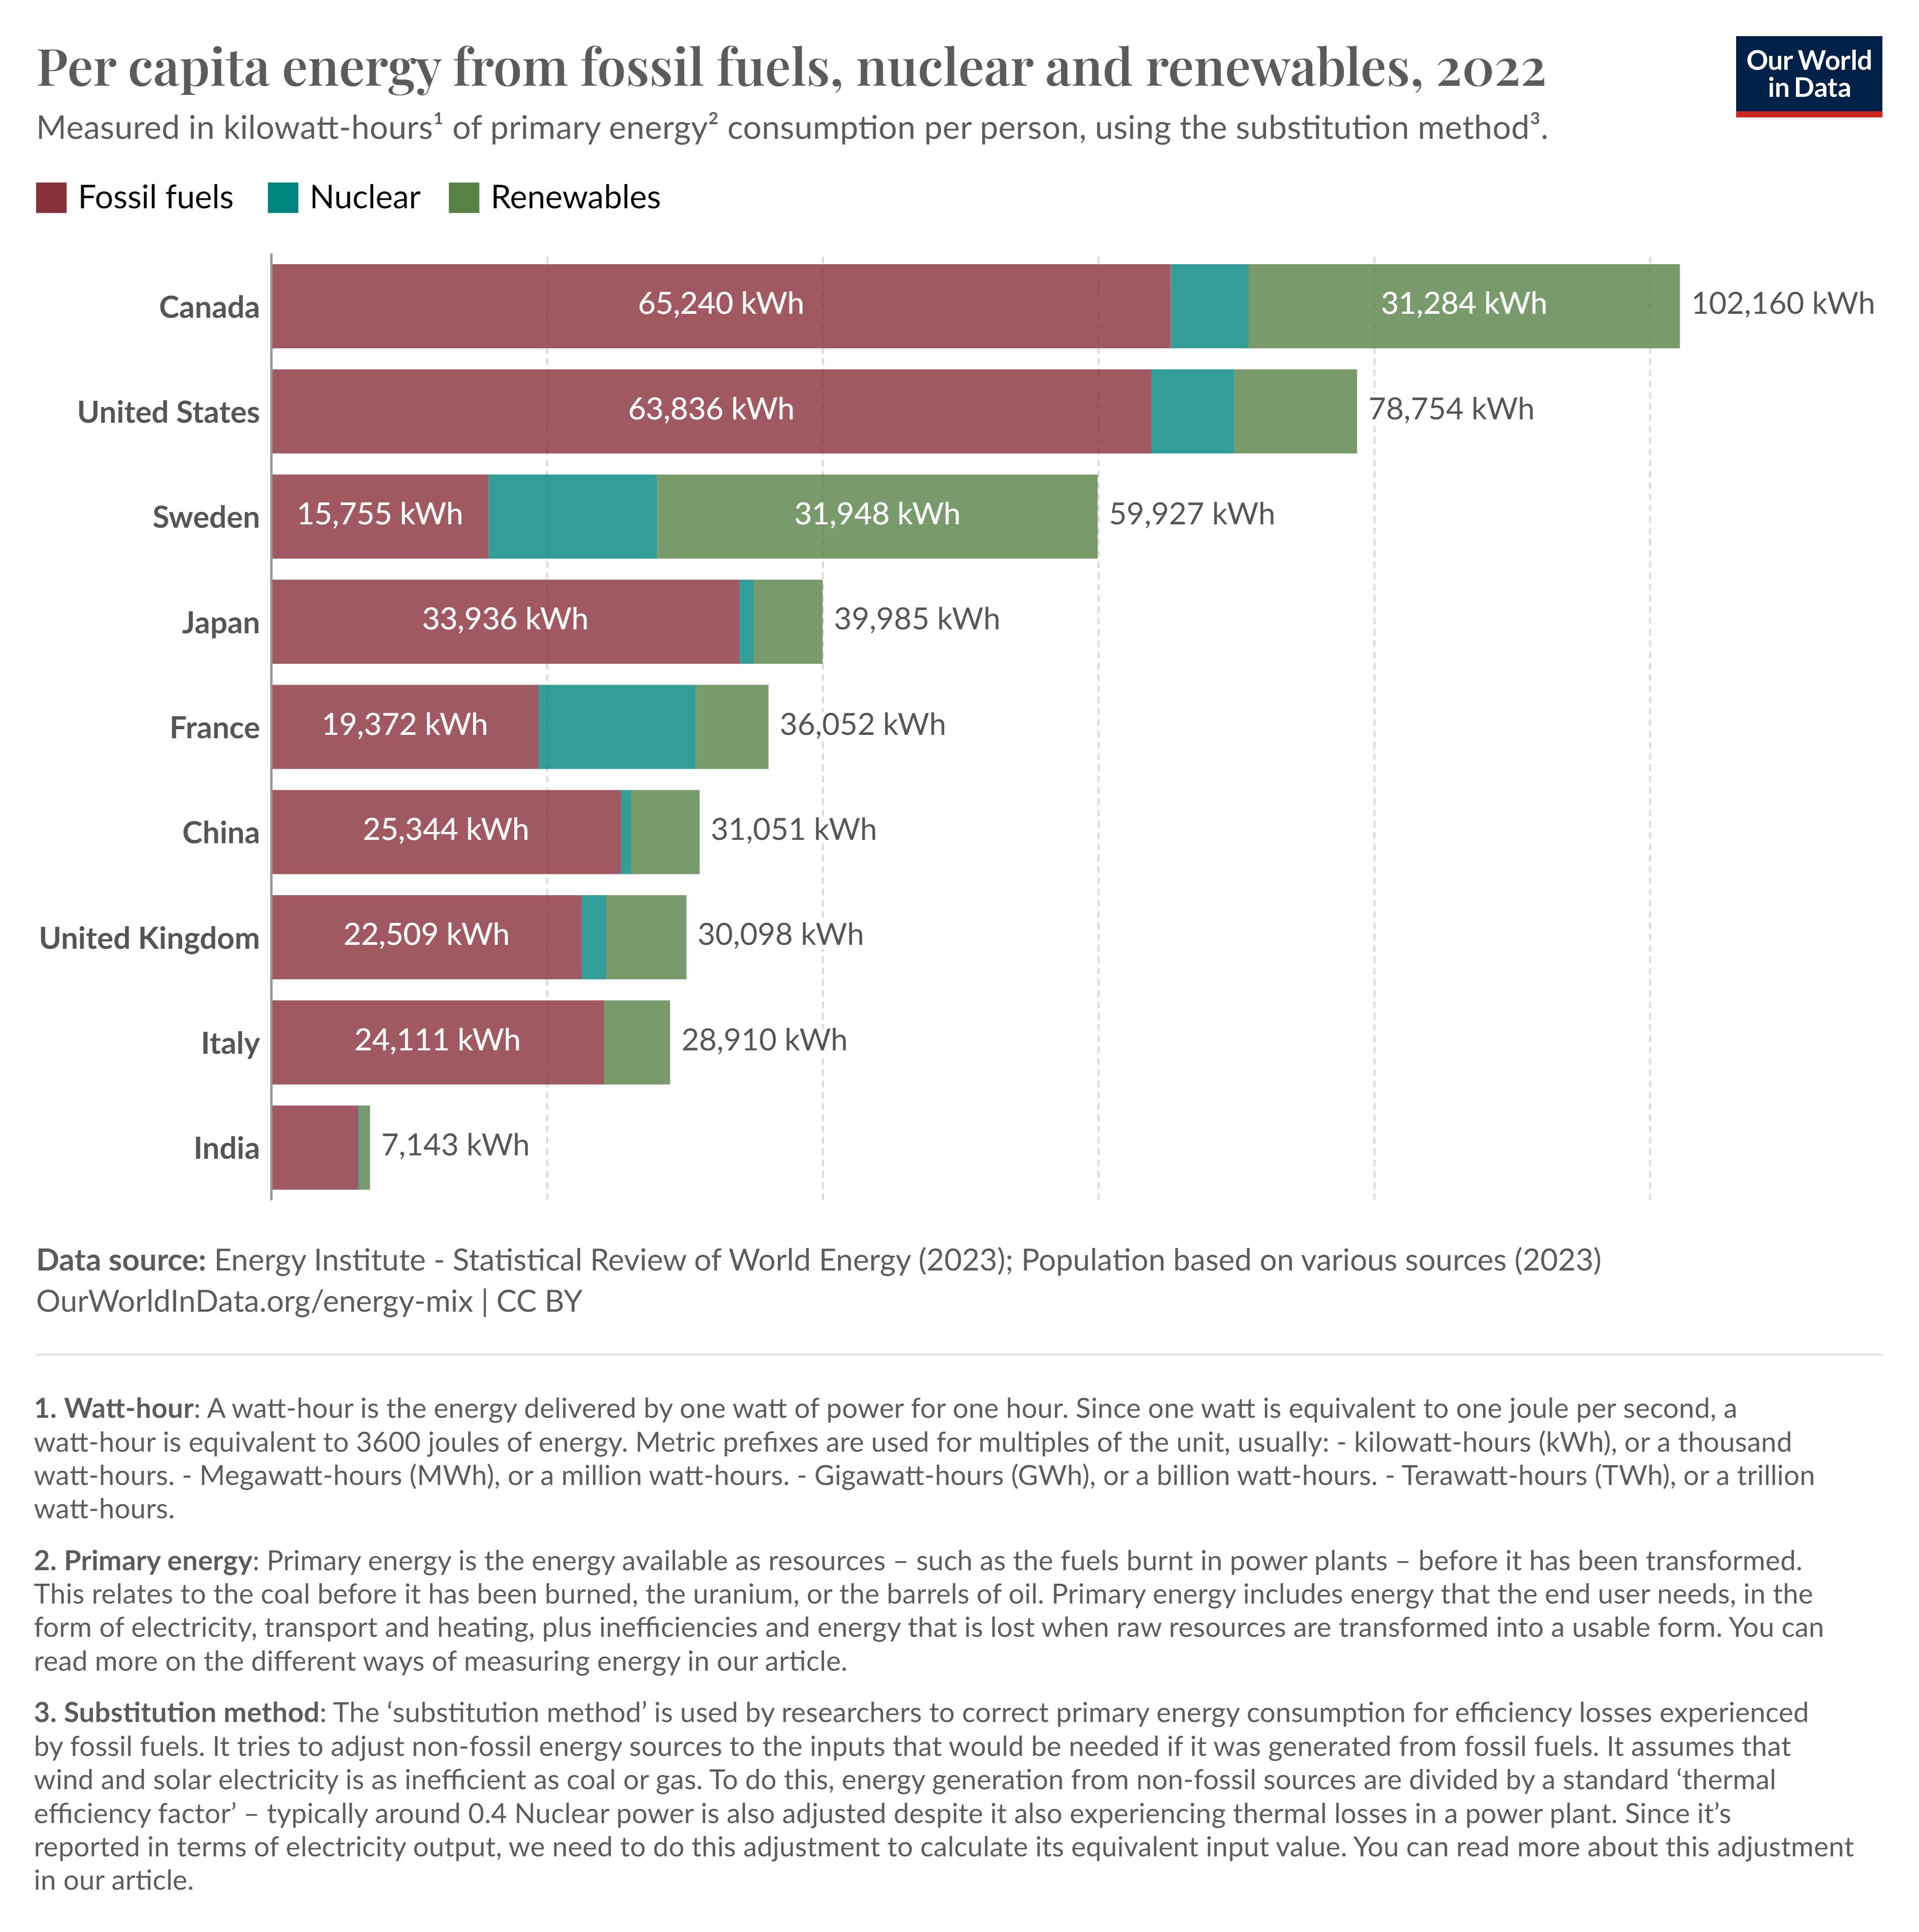
\includegraphics[scale=0.1]{images/per-capita-energy-source-stacked.png}
    \caption{Fonti di energia per paese}
\end{figure}

\noindent Come si può vedere dal grafico \cite{energy-mix} le fonti di energia variano da paese a paese e quindi il CI varia a seconda del paese in cui si esegue l'attività. Questo è un aspetto molto importante nel caso di addestramento sostenibile. A parità di energia consumata un modello addestrato in un paese con una fonte di energia più pulita avrà un impatto ambientale minore rispetto ad un modello addestrato in un paese con una fonte di energia più inquinante.\\

    \newpage
    \section{Esperimenti}

\subsection{Dataset utilizzati}
\subsubsection{LFM1b}


LFM1b\_artist è un dataset contenente informazioni riguardanti le interazioni tra utenti e artisti musicali.

\noindent Descrizione del dataset
\begin{table}[H]
    \centering
    \footnotesize
    \begin{tabularx}{\textwidth}{|c|X|}
        \hline
        \textbf{Feature} & \textbf{Descrizione} \\
        \hline
        n\_users & 120322 \\
        \hline
        n\_items & 3123496 \\
        \hline
        n\_inter & 65133026 \\
        \hline
        sparsity & 0.9998266933373666 \\
        \hline
        avg\_inter\_user & 541.3226675088513 \\
        \hline
    \end{tabularx}
    \caption{Informazioni sul dataset LFM1b\_artist}
    \label{tab:dataset_info}
\end{table}


\noindent Descrizione del knowledge graph
\begin{table}[H]
    \centering
    \footnotesize
    \begin{tabularx}{\textwidth}{|c|X|}
        \hline
        n\_ent\_head & 823213 \\
        \hline
        n\_ent\_tail & 353607 \\
        \hline
        n\_rel & 8 \\
        \hline
        n\_triple & 2114049 \\
        \hline
    \end{tabularx}
    \caption{Informazioni sul knowledge graph del dataset LFM1b\_artist}
    \label{tab:dataset_info}
\end{table}



\paragraph{Descrizione procedimento di pre-processing}


\noindent Il dataset originale risultava essere troppo grande per le risorse a nostra disposizione, dunque è stato opportunamente processato. In paritcolare sono state svolte le seguenti operazioni
\begin{itemize}
    \item \textbf{Filtraggio:} il dataset è stato filtrato eliminando tutte le interazioni in cui erano coinvolti utenti e/o item con meno di 5 interazioni
    \item \textbf{Sampling:} dopo la fase di filtraggio, è stato effettuato un sampling casuale il cui scopo era quello di ridurre il numero di utenti e di item presenti. In particolare sono stati selezionati casualmente 20000 utenti e 50000 item e sono state mantenute solo le interazioni in cui erano coinvolti utenti e item selezionati
\end{itemize}

\noindent In questo modo è stato ottenuto un dataset più piccolo e più facilmente gestibile rispetto a quello originale.
Per poter lavorare su più dataset si è deciso di effettuare un ulteriore processing del dataset, andando a creare dei sampling con una strategia di stratificazione: \footnote{{{Mantenendo il numero di utenti inalterato per ognuno di essi sono stati campionati casualmente un determinato numero di interazioni cercando di mantenere inalterati i "rapporti originali" tra i diversi utenti}}}{}
\begin{itemize}
    \item \textbf{75\%:} Per ogni utente sono state mantenute il 75\% delle interazioni originali
    \item \textbf{50\%:} Dal dataset al 75\% sono state mantenute circa il 66.67\% delle interazioni di ogni utente, in modo tale da avere il 50\% delle interazioni originali
    \item \textbf{25\%:} Dal dataset al 50\% sono state mantenute il 50\% delle interazioni di ogni utente, in modo tale da avere il 25\% delle interazioni originali
\end{itemize}


\noindent\textbf{Dataset 20.000 users, 50.000 items}

\noindent Descrizione del dataset
\begin{table}[H]
    \centering
    \footnotesize
    \begin{tabularx}{\textwidth}{|c|X|}
        \hline
        \textbf{Feature} & \textbf{Descrizione} \\
        \hline
        n\_users & 19841 \\
        \hline
        n\_items & 42457 \\
        \hline
        n\_inter & 900212 \\
        \hline
        sparsity & 0.9989313587429705 \\
        \hline
        avg\_inter\_user & 45.371301849705155 \\
        \hline
    \end{tabularx}
    \caption{Informazioni sul dataset LFM1b\_artist\_20U50I}
    \label{tab:dataset_info}
\end{table}


\noindent Descrizione del knowledge graph
\begin{table}[H]
    \centering
    \footnotesize
    \begin{tabularx}{\textwidth}{|c|X|}
        \hline
        n\_ent\_head & 15509 \\
        \hline
        n\_ent\_tail & 35156 \\
        \hline
        n\_rel & 5 \\
        \hline
        n\_triple & 46827 \\
        \hline
    \end{tabularx}
    \caption{Informazioni sul knowledge graph del dataset LFM1b\_artist\_20U50I}
    \label{tab:dataset_info}
\end{table}

\noindent\textbf{Dataset 75\%}

\noindent Descrizione del dataset
\begin{table}[H]
    \centering
    \footnotesize
    \begin{tabularx}{\textwidth}{|c|X|}
        \hline
        \textbf{Feature} & \textbf{Descrizione} \\
        \hline
        n\_users & 19841 \\
        \hline
        n\_items & 38932 \\
        \hline
        n\_inter & 667850 \\
        \hline
        sparsity & 0.9991354130849345 \\
        \hline
        avg\_inter\_user & 33.660097777329774 \\
        \hline
    \end{tabularx}
    \caption{Informazioni sul dataset LFM1b\_artist\_20U50I\_75strat}
    \label{tab:dataset_info}
\end{table}


\noindent Descrizione del knowledge graph
\begin{table}[H]
    \centering
    \footnotesize
    \begin{tabularx}{\textwidth}{|c|X|}
        \hline
        n\_ent\_head & 14327 \\
        \hline
        n\_ent\_tail & 32981 \\
        \hline
        n\_rel & 5 \\
        \hline
        n\_triple & 43559 \\
        \hline
    \end{tabularx}
    \caption{Informazioni sul knowledge graph del dataset LFM1b\_artist\_20U50I\_75strat}
    \label{tab:dataset_info}
\end{table}

\noindent\textbf{Dataset 50\%}

\noindent Descrizione del dataset
\begin{table}[H]
    \centering
    \footnotesize
    \begin{tabularx}{\textwidth}{|c|X|}
        \hline
        \textbf{Feature} & \textbf{Descrizione} \\
        \hline
        n\_users & 19841 \\
        \hline
        n\_items & 33653 \\
        \hline
        n\_inter & 440620 \\
        \hline
        sparsity &  0.9993401019218887 \\
        \hline
        avg\_inter\_user & 22.20755002268031 \\
        \hline
    \end{tabularx}
    \caption{Informazioni sul dataset LFM1b\_artist\_20U50I\_50strat}
    \label{tab:dataset_info}
\end{table}


\noindent Descrizione del knowledge graph
\begin{table}[H]
    \centering
    \footnotesize
    \begin{tabularx}{\textwidth}{|c|X|}
        \hline
        n\_ent\_head & 12522 \\
        \hline
        n\_ent\_tail & 29509 \\
        \hline
        n\_rel & 5 \\
        \hline
        n\_triple & 38491 \\
        \hline
    \end{tabularx}
    \caption{Informazioni sul knowledge graph del dataset LFM1b\_artist\_20U50I\_50strat}
    \label{tab:dataset_info}
\end{table}

\noindent\textbf{Dataset 25\%}

\noindent Descrizione del dataset
\begin{table}[H]
    \centering
    \footnotesize
    \begin{tabularx}{\textwidth}{|c|X|}
        \hline
        \textbf{Feature} & \textbf{Descrizione} \\
        \hline
        n\_users & 19841 \\
        \hline
        n\_items & 24878 \\
        \hline
        n\_inter & 218457 \\
        \hline
        sparsity & 0.9995574249320202 \\
        \hline
        avg\_inter\_user & 11.01038254120256 \\
        \hline
    \end{tabularx}
    \caption{Informazioni sul dataset LFM1b\_artist\_20U50I\_25strat}
    \label{tab:dataset_info}
\end{table}


\noindent Descrizione del knowledge graph
\begin{table}[H]
    \centering
    \footnotesize
    \begin{tabularx}{\textwidth}{|c|X|}
        \hline
        n\_ent\_head & 9444 \\
        \hline
        n\_ent\_tail & 23463 \\
        \hline
        n\_rel & 5 \\
        \hline
        n\_triple & 29822 \\
        \hline
    \end{tabularx}
    \caption{Informazioni sul knowledge graph del dataset LFM1b\_artist\_20U50I\_25strat}
    \label{tab:dataset_info}
\end{table}

\subsubsection{Movielens-10m}
\noindent MovieLens10M è la versione a 10 milioni di interazioni del dataset MovieLens. In questo caso è stato aggiunto anche un KG con un hop pari a 1

\noindent Descrizione del dataset
\begin{table}[H]
    \centering
    \footnotesize
    \begin{tabularx}{\textwidth}{|c|X|}
        \hline
        \textbf{Feature} & \textbf{Descrizione} \\
        \hline
        n\_users & 69878 \\
        \hline
        n\_items & 10677 \\
        \hline
        n\_inter & 10000054 \\
        \hline
        sparsity & 0.9865966722939162 \\
        \hline
        avg\_inter\_user & 143.10732991785684 \\
        \hline
    \end{tabularx}
    \caption{Informazioni sul dataset ml-10m}
    \label{tab:dataset_info}
\end{table}


\noindent Descrizione del knowledge graph
\begin{table}[H]
    \centering
    \footnotesize
    \begin{tabularx}{\textwidth}{|c|X|}
        \hline
        n\_ent\_head & 179775 \\
        \hline
        n\_ent\_tail & 181868 \\
        \hline
        n\_rel & 49 \\
        \hline
        n\_triple & 1051385 \\
        \hline
    \end{tabularx}
    \caption{Informazioni sul knowledge graph del dataset ml-10m}
    \label{tab:dataset_info}
\end{table}




\paragraph{Descrizione procedimento di pre-processing}


\noindent Il dataset originale risultava essere troppo grande per le risorse a nostra disposizione, dunque è stato opportunamente processato. In paritcolare sono state svolte le seguenti operazioni
\begin{itemize}
    \item \textbf{Filtraggio:} il dataset è stato filtrato eliminando tutte le interazioni in cui erano coinvolti utenti e/o item con meno di 5 interazioni
    \item \textbf{Sampling:} dopo la fase di filtraggio, è stato effettuato un sampling casuale il cui scopo era quello di ridurre il numero di utenti e di item presenti. In particolare sono stati selezionati casualmente 50000 utenti e 10000 item e sono state mantenute solo le interazioni in cui erano coinvolti utenti e item selezionati
\end{itemize}

\noindent In questo modo è stato ottenuto un dataset più piccolo e più facilmente gestibile rispetto a quello originale.

\noindent\textbf{Dataset con 50.000 utenti e 10.000 items}

\noindent Descrizione del dataset
\begin{table}[H]
    \centering
    \footnotesize
    \begin{tabularx}{\textwidth}{|c|X|}
        \hline
        \textbf{Feature} & \textbf{Descrizione} \\
        \hline
        n\_users & 50000 \\
        \hline
        n\_items & 10000 \\
        \hline
        n\_inter & 7053774 \\
        \hline
        sparsity & 0.985892452 \\
        \hline
        avg\_inter\_user & 141.07548 \\
        \hline
    \end{tabularx}
    \caption{Informazioni sul dataset ml-10m\_50U10I}
    \label{tab:dataset_info}
\end{table}


\noindent Descrizione del knowledge graph
\begin{table}[H]
    \centering
    \footnotesize
    \begin{tabularx}{\textwidth}{|c|X|}
        \hline
        n\_ent\_head & 9937 \\
        \hline
        n\_ent\_tail & 167042 \\
        \hline
        n\_rel & 31 \\
        \hline
        n\_triple & 521125 \\
        \hline
    \end{tabularx}
    \caption{Informazioni sul knowledge graph del dataset ml-10m\_50U10I}
    \label{tab:dataset_info}
\end{table}


\subsubsection{Movielens-1m}

\noindent MovieLens1M è la versione a 1 milione di interazioni del dataset MovieLens.

\noindent Descrizione del dataset
\begin{table}[H]
    \centering
    \footnotesize
    \begin{tabularx}{\textwidth}{|c|X|}
        \hline
        \textbf{Feature} & \textbf{Descrizione} \\
        \hline
        n\_users & 6040 \\
        \hline
        n\_items & 3706 \\
        \hline
        n\_inter & 1000209 \\
        \hline
        sparsity & 0.9553163743776871 \\
        \hline
        avg\_inter\_user & 165.5975165562914 \\
        \hline
    \end{tabularx}
    \caption{Informazioni sul dataset ml-1m}
    \label{tab:dataset_info}
\end{table}

\noindent Descrizione del knowledge graph
\begin{table}[H]
    \centering
    \footnotesize
    \begin{tabularx}{\textwidth}{|c|X|}
        \hline
        n\_ent\_head & 78314 \\
        \hline
        n\_ent\_tail & 79347 \\
        \hline
        n\_rel & 49 \\
        \hline
        n\_triple & 385923 \\
        \hline
    \end{tabularx}
    \caption{Informazioni sul knowledge graph del dataset ml-1m}
    \label{tab:dataset_info}
\end{table}


\subsubsection{Amazon-Book}

\noindent Amazon-Book è un dataset contenente informazioni riguardanti le interazioni tra utenti e libri.
In questo caso è stata usata direttamente una versione ridotta (quindi con pre-processing già effettuato) del dataset originale con un core di 60.

\noindent Descrizione del dataset
\begin{table}[H]
    \centering
    \footnotesize
    \begin{tabularx}{\textwidth}{|c|X|}
        \hline
        \textbf{Feature} & \textbf{Descrizione} \\
        \hline
        n\_users & 22155 \\
        \hline
        n\_items & 54458 \\
        \hline
        n\_inter & 1465871 \\
        \hline
        sparsity & 0.9987850390735069 \\
        \hline
        avg\_inter\_user & 66.16434213495825 \\
        \hline
    \end{tabularx}
    \caption{Informazioni sul dataset amazon\_books\_60core\_kg}
    \label{tab:dataset_info}
\end{table}

\noindent Descrizione del knowledge graph
\begin{table}[H]
    \centering
    \footnotesize
    \begin{tabularx}{\textwidth}{|c|X|}
        \hline
        n\_ent\_head & 26282 \\
        \hline
        n\_ent\_tail & 26300 \\
        \hline
        n\_rel & 16 \\
        \hline
        n\_triple & 96476 \\
        \hline
    \end{tabularx}
    \caption{Informazioni sul knowledge graph del dataset amazon\_books\_60core\_kg}
    \label{tab:dataset_info}
\end{table}


\subsection{Esperimenti svolti}
\subsubsection{Benchmarking dei modelli}

La fase di benchmarking consiste nel continuare le ricerche già svolte in questo campo per poter confermare oppure smentire i risultati già ottenuti in passato.\\
\begin{figure}[H]
    \centering
    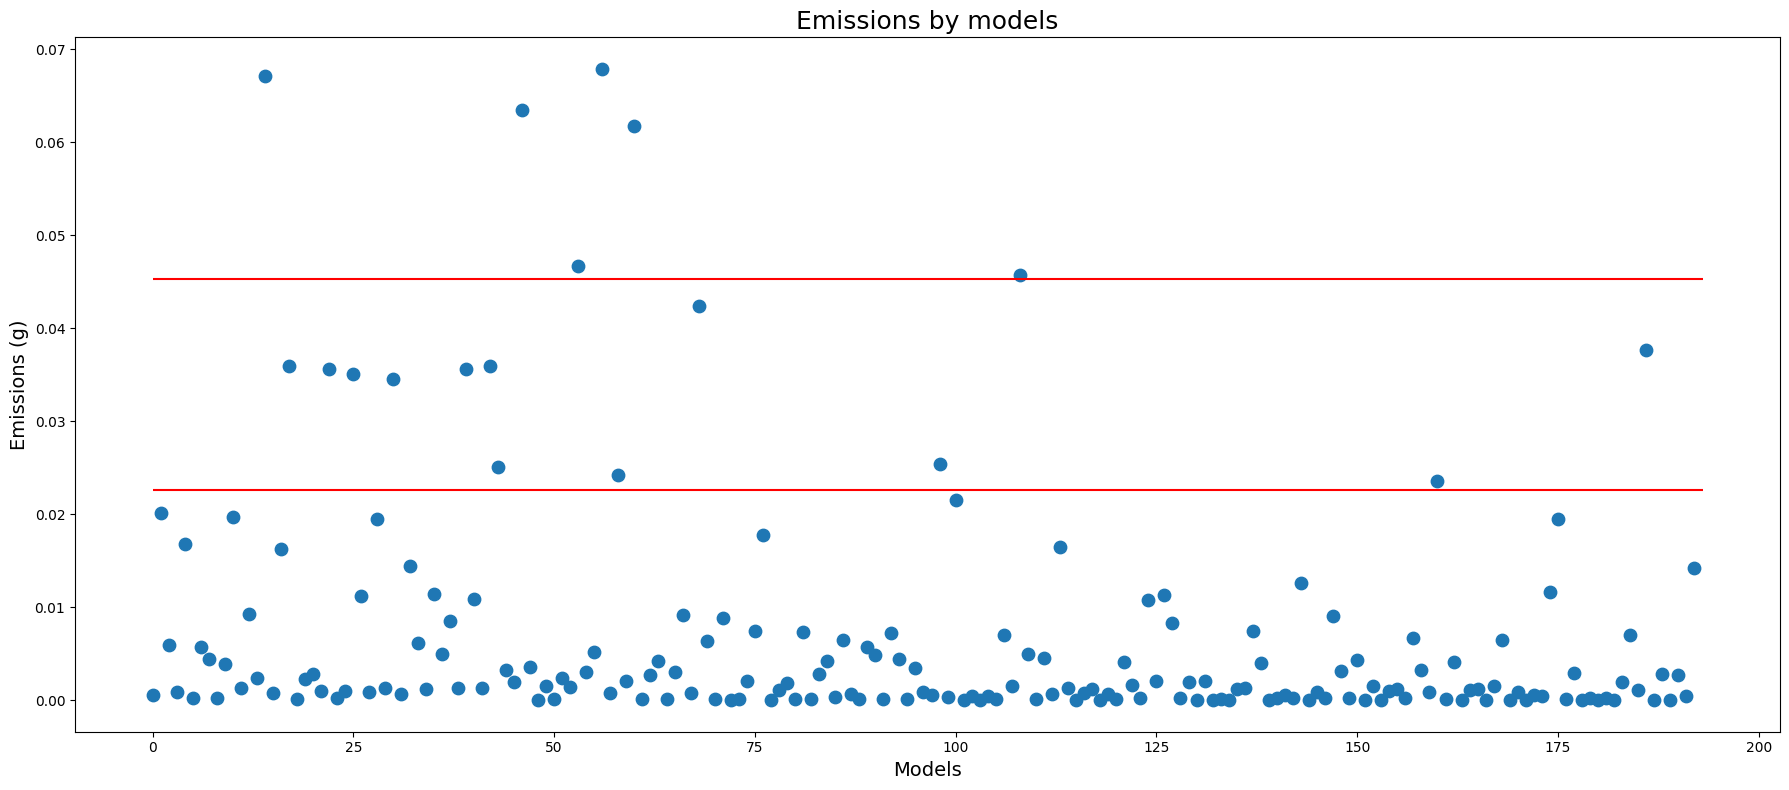
\includegraphics[width=\textwidth]{images/situazione-attuale.png}
    \caption{Emissioni prodotte dai vari modelli}
\end{figure}

\noindent Gli esperimenti passati sono stati condotti su dataset e modelli presenti all'interno di RecBole.\\I dataset utilizzati per l'addestramento dei modelli sono:
\begin{itemize}
    \item \textbf{MovieLens-1M}
    \item \textbf{Amazon\_Book\_60core\_kg} 
    \item \textbf{Mind}
\end{itemize}

\noindent I modelli utilizzati per l'addestramento sono:
\begin{itemize}
    \item \textbf{BPR} \cite{BPR}: General
    \item \textbf{CDAE} \cite{CDAE}: General
    \item \textbf{CFKG} \cite{CFKG}: Knowledge
    \item \textbf{CKE} \cite{CKE}: Knowledge
    \item \textbf{DGCF} \cite{DGCF}: Knowledge
    \item \textbf{DMF} \cite{DMF}: General
    \item \textbf{DiffRec} \cite{DiffRec}: General
    \item \textbf{ENMF} \cite{ENMF}: General 
    \item \textbf{FISM} \cite{FISM}: General
    \item \textbf{GCMC} \cite{GCMC}: General
    \item \textbf{ItemKNN} \cite{ItemKNN}: General
    \item \textbf{KGCN} \cite{KGCN}: Knowledge
    \item \textbf{KGIN}: \cite{KGIN} Knowledge
    \item \textbf{KGNNLS} \cite{KGNNLS}: Knowledge
    \item \textbf{KTUP} \cite{KTUP}: Knowledge
    \item \textbf{LDiffRec} \cite{LDiffRec}: General
    \item \textbf{LINE} \cite{LINE}: General
    \item \textbf{LightGCN} \cite{LightGCN}: General
    \item \textbf{MKR} \cite{MKR}: Knowledge
    \item \textbf{MacridVAE} \cite{MacridVAE}: General
    \item \textbf{MultiDAE} \cite{MultiDAE}: General
    \item \textbf{MultiVAE} \cite{MultiVAE}: General
    \item \textbf{NCEPLRec} \cite{NCEPLRec}: General
    \item \textbf{NCL} \cite{NCL}: General
    \item \textbf{NGCF} \cite{NGCF}: General
    \item \textbf{NeuMF} \cite{NeuMF}: General
    \item \textbf{Pop}: General
    \item \textbf{Random}: General
    \item \textbf{RecVAE} \cite{RecVAE}: General
    \item \textbf{RippleNet} \cite{RippleNet}: Knowledge
    \item \textbf{SGL} \cite{SGL}: General
    \item \textbf{SLIMElastic} \cite{SLIMElastic}: General
    \item \textbf{SimpleX} \cite{SimpleX}: General
    \item \textbf{SpectralCF} \cite{SpectralCF}: General
    \item \textbf{EASE} \cite{EASE}: General
    \item \textbf{NAIS} \cite{NAIS}: General
    \item \textbf{ADMMSLIM} \cite{ADMMSLIM}: General
    \item \textbf{ConvNCF} \cite{ConvNCF}: General
    \item \textbf{NNCF} \cite{NNCF}: General
\end{itemize}

\noindent In questo ambito  Spillo et al.\cite{spillo2023towards} mostrano come spesso algoritmi più semplici riescono ad avere delle performance molto simili a modelli più complessi, ma con un impatto ambientale decisamente minore. Lo scopo di questo lavoro è dunque quello di confermare o smentire questi risultati.\\
\begin{figure}[H]
    \centering
    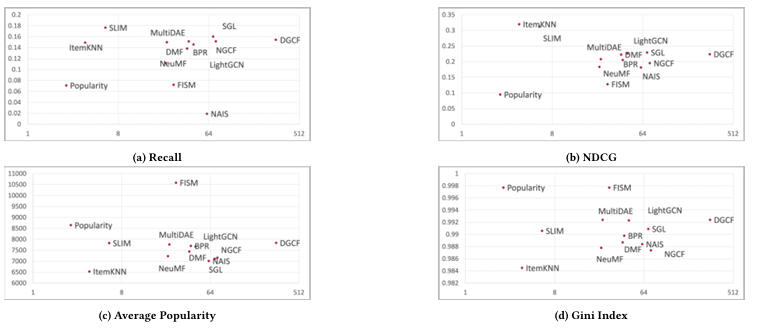
\includegraphics[width=\textwidth]{images/risultati-valutazione.png}
    \caption{Trade-off tra emissioni e performance con dataset Mind}
\end{figure}

\noindent RecBole richiede la definizione di un file di configurazione per poter addestrare i modelli. Questo file di configurazione contiene le seguenti informazioni:\\
\noindent \textbf{Parametri di environment} (servono per configurare l'ambiente di addestramento)
\begin{itemize}
    \item \textbf{gpu\_id}: 0
    \item \textbf{worker}: 0
    \item \textbf{use\_gpu}: True
    \item \textbf{seed}: 2020
    \item \textbf{state}: INFO
    \item \textbf{encoding}: utf-8
    \item \textbf{reproducibility}: True
    \item \textbf{shuffle}: True
\end{itemize}


\noindent \textbf{Parametri di training} (servono per l'addestramento dei modelli)
\begin{itemize}
    \item \textbf{epochs}: 200
    \item \textbf{train\_batch\_size}: 2048
    \item \textbf{learner}: adam
    \item \textbf{learning\_rate}: .001
    \item \textbf{train\_neg\_sample\_args}: 
    \begin{itemize}
        \item \textbf{distribution}: uniform
        \item \textbf{sample\_num}: 1
        \item \textbf{dynamic}: False
        \item \textbf{candidate\_num}: 0
    \end{itemize}
    \item \textbf{eval\_step}: 1
    \item \textbf{stopping\_step}: 10
    \item \textbf{clip\_grad\_norm}: None
    \item \textbf{loss\_decimal\_place}: 4
    \item \textbf{weight\_decay}: .0
    \item \textbf{require\_pow}: False
    \item \textbf{enable\_amp}: False
    \item \textbf{enable\_scaler}: False
\end{itemize}


\noindent \textbf{Parametri di evaluation} (servono per valutare i modelli)


\begin{itemize}
    \item \textbf{eval\_args}:
    \item \begin{itemize}
                \item \textbf{group\_by}: user
                \item \textbf{order}: RO
                \item \textbf{split}: RS : [0.8, 0.1, 0.1]
                \item \textbf{mode}: full
            \end{itemize}
    \item \textbf{repeatable}: False
    \item \textbf{metrics}: ['Recall', 'MRR', 'NDCG', 'Hit', 'MAP', 'Precision', 'GAUC', 'ItemCoverage', 'AveragePopularity', 'GiniIndex', 'ShannonEntropy', 'TailPercentage']
    \item \textbf{topk}: 10
    \item \textbf{valid\_metric}: MRR@10
    \item \textbf{eval\_batch\_size}: 4096
    \item \textbf{metric\_decimal\_place}: 4
\end{itemize}


\noindent \textbf{Iper parametri dei modelli}


\noindent Gli iper parametri dei modelli sono un insieme di parametri che vengono utilizzati per configurare i modelli. La loro configurazione può influenzare il risultato finale. Esistono delle tecniche di HyperTuning che permettono di trovare i migliori iper parametri per un determinato modello e dataset.
In questo caso si è scelto di utilizzare gli iper parametri di default per tutti i modelli.\\Per ognuno dei modelli SOTA scelti (prima elencati) sono stati effettuati run con i seguenti dataset:
\begin{itemize}
    \item \textbf{LFM1b\_artist\_20U50I}
    \item \textbf{LFM1b\_artist\_20U50I\_75strat}
    \item \textbf{LFM1b\_artist\_20U50I\_50strat}
    \item \textbf{LFM1b\_artist\_20U50I\_25strat}
    \item \textbf{ml-10m\_50U10I}
\end{itemize}

\noindent Dopo aver terminato le esecuzioni dei modelli sono stati creati dei grafici per poter confrontare i risultati ottenuti. I grafici sono i due tipi:
\begin{itemize}
    \item \textbf{Grafici a barre:} Questi grafici permettono di confrontare le emissioni dei vari modelli rispetto a ogni dataset.
    \item \textbf{Grafici a dispersione:} Questi dataset permettono di confrontare i trade-off tra emissioni e performance dei vari modelli rispetto a ogni dataset.
\end{itemize}

\noindent Per la valutazione dei modelli sono state utilizzate le seguenti metriche:
\begin{itemize}
    \item \textbf{Recall}: è una metrica che misura la capacità di un modello di raccomandare gli item rilevanti per un utente
    \item \textbf{NDCG}: è una metrica che misura la qualità delle raccomandazioni.
    \item \textbf{Gini Index}: è una metrica che misura l'equità nella distribuzione delle raccomandazioni. Un valore più vicino a zero indica una distribuzione più equa
    \item \textbf{Average Popularity}: è una metrica che misura la popolarità media degli item raccomandati. Un valore alto indica che le raccomandazioni sono concentrate su item popolari.
\end{itemize}



\subsubsection{Addestramento sostenibile}
L'addestramento sostenibile consiste nell'addestrare i modelli di recommendation in modo sostenibile, ovvero cercando di ridurre le emissioni di CO2 prodotte durante l'addestramento senza compromettere le performance dei modelli in modo significativo.
Si è dunque deciso di modificare il criterio di early stopping dei modelli inserendo come variabile anche le emissioni.
Il classico criterio di early stopping prevede di fermare l'addestramento del modello quando lo score ottenuto con il validation set non migliora per un certo numero di epoche consecutive.


\begin{figure}[H]
    \centering
     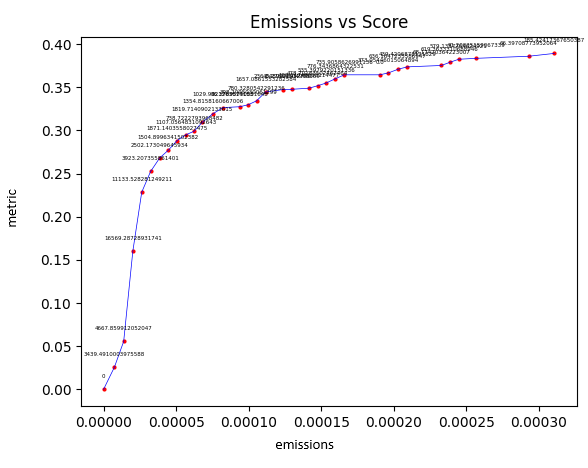
\includegraphics[width=\textwidth]{images/curve_emissions_score.png}
    \caption{Andamento dello score in funzione delle emissioni}
\end{figure}

\noindent Questa curva mostra mostra il comportamento dello score in funzione delle emissioni. In particolare si tiene traccia solo delle epoche in cui lo score è migliorato rispetto al risultato migliore.
Si può notare come la curva presenti una forte crescita iniziale, per poi stabilizzarsi e avere un andamento quasi lineare.
Questo andamento lineare indica dunque un miglioramento molto piccolo dello score rispetto all'aumento delle emissioni.

\noindent Il criterio di early stopping con emissioni si pone dunque come obiettivo quello di fermare l'addestramento del modello quando il miglioramento dello score rispetto alle emissioni è troppo piccolo.
L'idea alla base sarebbe quello di fermare l'addestramento studiando la derivata della curva. Siccome i valori sono discreti, si è deciso di approssimare la derivata con la differenza tra due punti consecutivi \footnote{Metodo delle differenze divise di ordine 1}{} mediante la seguente formula:
\begin{equation}
    \frac{f(x_{i+1}) - f(x_i)}{x_{i+1} - x_i}
\end{equation}

\noindent Quando la differenza tra due rapporti consecutivi è minore di una certa soglia, per un certo numero di volte consecutive, si ferma l'addestramento del modello.\\
\paragraph{Parte esplorativa}
In questa parte si sono eseguti diversi esperimenti usando dataset diversi e parametri diversi per cercare di capire come il criterio di early stopping con emissioni influenzi le performance dei modelli in base ai parametri e alle dimensioni del dataset.\\
\begin{itemize}
    \item \textbf{Primo esperimento}: è stato eseguito con il dataset MovieLens-1m. La soglia è stata impostata a 50 e il numero di epoche consecutive a 5.
    \item \textbf{Secondo esperimento}: è stato eseguito con il dataset LFM-1b\_artist\_20U50I\_25strat. La soglia è stata impostata a 30 e il numero di epoche consecutive a 7, dunque un criterio più stringente (una differenza tra i rapporti consecutivi minore da verificare per più miglioramenti consecutivi).
    \item \textbf{Terzo esperimento}: è stato eseguito sul dataset amazon\_books\_60core\_kg e i parametri utilizzati sono stati 40 come soglia e 6 come numero di epoche consecutive, dunque una via di mezzo tra i due esperimenti precedenti.
\end{itemize}

Per ogni esperimento sono stati realizzati i seguenti grafici:
\begin{itemize}
    \item \textbf{Grafico delle emissioni}: confronta le emissioni prodotte dai vari modelli durante l'addestramento.
    \item \textbf{Grafico del trade-off}: mette in relazione il trade-off tra emissioni e performance dei modelli addestrati con il criterio di early stopping con emissioni e il trade-off dei modelli addestrati con il criterio di early stopping classico.
    \item \textbf{Grafico del decrementi performance}: mostra il decremento delle performance dei modelli addestrati con il criterio di early stopping con emissioni rispetto al criterio di early stopping classico.
\end{itemize}

Anche in questo caso sono state utilizzate le seguenti metriche per valutare i modelli:
\begin{itemize}
    \item \textbf{Recall}
    \item \textbf{NDCG}
    \item \textbf{Gini Index}
    \item \textbf{Average Popularity}
\end{itemize}

\paragraph{Confronto tra i criteri di early stopping con emissioni}
In questa parte parte si è cercato di capire come i parametri del criterio di early stopping con emissioni influenzino le performance dei modelli.\\
Per fare ciò si è deciso di eseguire un esperimento con il dataset MovieLens-1m e di variare i parametri del criterio di early stopping con emissioni.\\
Gli esperimenti eseguti sono stati i seguenti:
\begin{itemize}
    \item \textbf{Primo esperimento}: è stato eseguito con la soglia impostata a 40 e il numero di epoche consecutive a 5.
    \item \textbf{Secondo esperimento}: è stato eseguito con la soglia impostata a 30 e il numero di epoche consecutive a 5.
    \item \textbf{Terzo esperimento}: è stato eseguito con la soglia impostata a 40 e il numero di epoche consecutive a 6.
    \item \textbf{Quarto esperimento}: è stato eseguito con la soglia impostata a 30 e il numero di epoche consecutive a 6.
    \item \textbf{Quinto esperimento}: è stato eseguito con la soglia impostata a 40 e il numero di epoche consecutive a 7.
    \item \textbf{Sesto esperimento}: è stato eseguito con la soglia impostata a 30 e il numero di epoche consecutive a 7.
\end{itemize}

\noindent Sono stati prodotti gli stessi grafici degli esperimenti precedenti per poter confrontare i risultati ottenuti. Sono state utilizzate le stesse metriche degli esperimenti precedenti per valutare i modelli.

\paragraph{Studio della sensibilità dei parametri}
\noindent Per poter confrontare i risultati ottenuti e come i parametri influenzino le performance dei modelli sono stati realizzati dei grafici che mettono in relazione i trade-off tra emissioni e performance dei modelli addestrati con i diversi parametri del criterio di early stopping con emissioni, in modo da osservare la sensibilità dei parametri.

    \newpage
    \section{Discussione}

\subsection{Benchmarking}

\subsubsection{Emissioni}
Qui di seguito vengono riportate le emissioni di CO2 per ogni esperimento effettuato.

\paragraph{LFM-1b\_artist} \textcolor{white}{.} \\
\begin{table}[H]
    \centering
    \footnotesize
    \setlength\tabcolsep{0pt}
    \begin{tabularx}{\textwidth}{|X|X|}
        \hline
        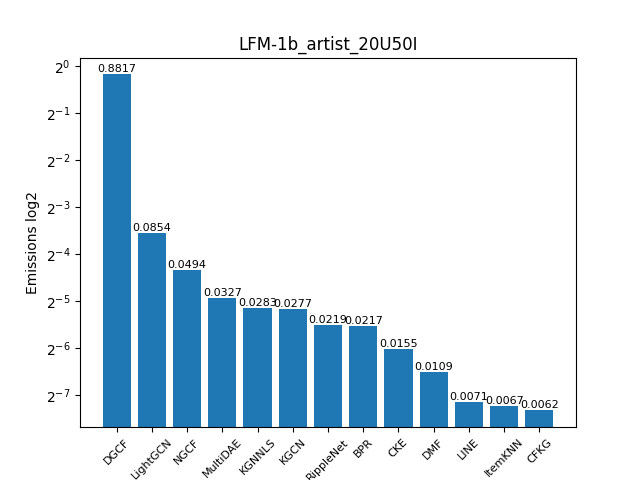
\includegraphics[width=\linewidth, trim=0 0 0 0]{images/emissions_LFM-1b_artist_20U50I.png} &
        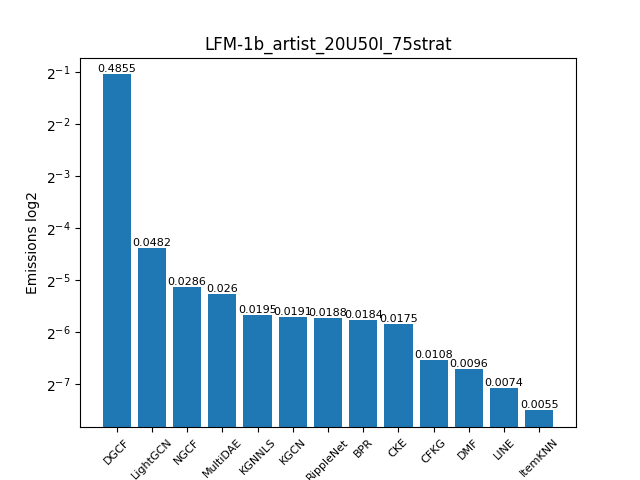
\includegraphics[width=\linewidth, trim=0 0 0 0]{images/emissions_LFM-1b_artist_20U50I_75strat.png} \\
        \hline
        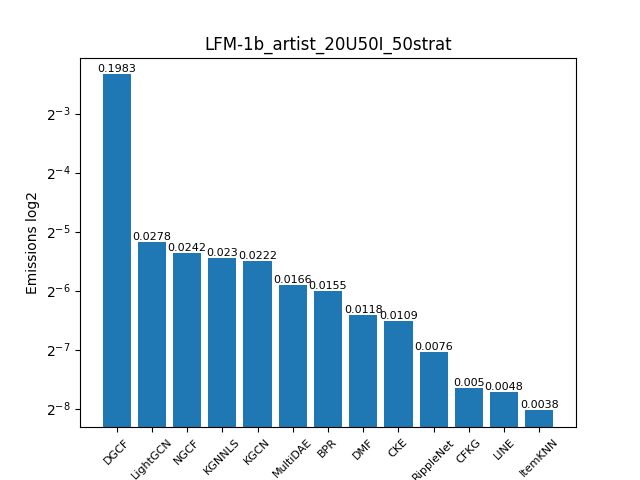
\includegraphics[width=\linewidth, trim=0 0 0 0]{images/emissions_LFM-1b_artist_20U50I_50strat.png} &
        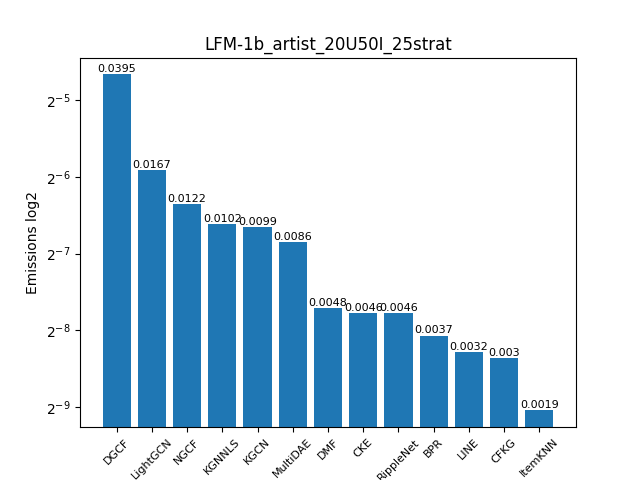
\includegraphics[width=\linewidth, trim=0 0 0 0]{images/emissions_LFM-1b_artist_20U50I_25strat.png} \\
        \hline
    \end{tabularx}
    \caption{Emissioni di CO2 per i vari dataset LFM-1b}
    \label{tab:emissions_info}
\end{table}

\noindent Si può subito notare come DGCF è il modello che emette più CO2 in assoluto.
In particolare con il dataset al 100\% e al 75\% DGCF emette circa 10 volte di più rispetto a LightGCN (il secondo per emissioni)
mentre con il dataset al 50\% emette circa 7 volte di più e con il dataset al 25\% emette circa 2 volte di più (sempre rispetto a LightGCN).
LightGCN e NCFG sono rispettivamente il secondo e il terzo modello che emettono più CO2.
Questi due modelli sono di tipo general, ma nonostante ciò emettono di più rispetto ad altri di tipo knowledge-aware, come per esempio il KGCN.
In generale possiamo vedere che ItemKNN,LINE e CFKG sono i modelli che emettono meno.
Per LINE e ItemKNN questo era abbastanza prevedibile in quanto modelli di tipo General. Interessante invece notare come CFKG, di tipo knowledge-aware, emetta meno di altri modelli di tipo General

\paragraph{MovieLens-10M\_50U10I} \textcolor{white}{.} \\
\begin{figure}[H]
    \centering
    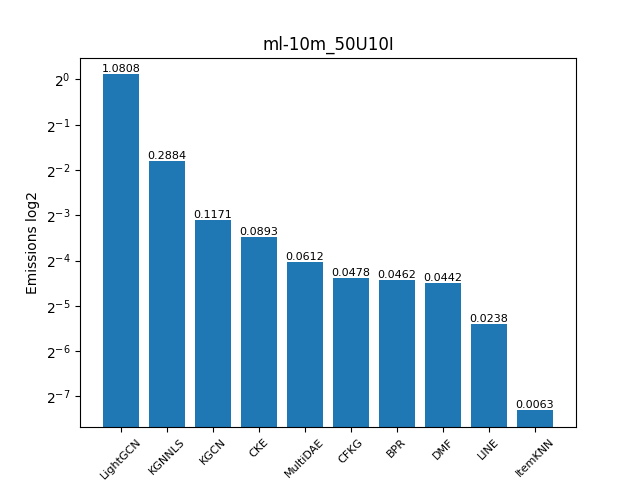
\includegraphics[scale=0.75]{images/emissions_ml-10m_50U10I.png}
    \caption{Emissioni di CO2 per il dataset MovieLens-10M\_50U10I}
\end{figure}

\noindent Si può subito notare come DGCF è il modello che emette più CO2 in assoluto.
In particolare con il dataset al 100\% e al 75\% DGCF emette circa 10 volte di più rispetto a LightGCN (il secondo per emissioni)
mentre con il dataset al 50\% emette circa 7 volte di più e con il dataset al 25\% emette circa 2 volte di più (sempre rispetto a LightGCN).
LightGCN e NCFG sono rispettivamente il secondo e il terzo modello che emettono più CO2.
Questi due modelli sono di tipo general, ma nonostante ciò emettono di più rispetto ad altri di tipo knowledge-aware, come per esempio il KGCN.
In generale possiamo vedere che ItemKNN,LINE e CFKG sono i modelli che emettono meno.
Per LINE e ItemKNN questo era abbastanza prevedibile in quanto modelli di tipo General. Interessante invece notare come CFKG, di tipo knowledge-aware, emetta meno di altri modelli di tipo General

\subsubsection{Trade-off}

In questa sezione verranno analizzati i trade-off tra le varie metriche di valutazione e le emissioni di CO2 analizzando un dataset per volta.

\paragraph{LFM-1b\_artist\_20U50I} \textcolor{white}{.} \\
\begin{table}[H]
    \centering
    \footnotesize
    \setlength\tabcolsep{0pt}
    \begin{tabularx}{\textwidth}{|X|X|}
        \hline
        \includegraphics[width=\linewidth, trim=0 0 0 0]{images/recall@10\_LFM-1b\_artist_20U50I.png} &
        \includegraphics[width=\linewidth, trim=0 0 0 0]{images/ndcg@10\_LFM-1b\_artist_20U50I.png} \\
        \hline
        \includegraphics[width=\linewidth, trim=0 0 0 0]{images/giniindex@10\_LFM-1b\_artist_20U50I.png} &
        \includegraphics[width=\linewidth, trim=0 0 0 0]{images/averagepopularity@10\_LFM-1b\_artist_20U50I.png} \\
        \hline
    \end{tabularx}
    \caption{Trade-off con il dataset LFM-1b\_artist\_20U50I}
    \label{tab:emissions_info}
\end{table}

\noindent Come già visto precedentemente, DGCF è il modello che emette di più. Nonostante ciò possiamo notare che per la recall e l'ndcg le sue performance risultano peggiori rispetto ad algoritmi più semplici come l'ItemKNN che risulta essere uno degli algoritmi che emette meno e performa meglio in queste metriche.
Per quanto riguarda il Gini Index possiamo notare che DGCF si comporta meglio di molti altri modelli ma l'ItemKNN e LINE risultano essere migliori di quest'ultimo. LINE è il miglior algoritmo.
Infine, per quanto riguarda l'Average Popularity, anche in questo caso possiamo notare anche che DGCF performa meglio di altri modelli, ma LINE risulta il miglior in assoluto ed è uno degli algoritmi che emette meno.

\paragraph{LFM-1b\_artist\_20U50I\_75strat} \textcolor{white}{.} \\
\begin{table}[H]
    \centering
    \footnotesize
    \setlength\tabcolsep{0pt}
    \begin{tabularx}{\textwidth}{|X|X|}
        \hline
        \includegraphics[width=\linewidth, trim=0 0 0 0]{images/recall@10\_LFM-1b\_artist_20U50I\_75strat.png} &
        \includegraphics[width=\linewidth, trim=0 0 0 0]{images/ndcg@10\_LFM-1b\_artist_20U50I\_75strat.png} \\
        \hline
        \includegraphics[width=\linewidth, trim=0 0 0 0]{images/giniindex@10\_LFM-1b\_artist_20U50I\_75strat.png} &
        \includegraphics[width=\linewidth, trim=0 0 0 0]{images/averagepopularity@10\_LFM-1b\_artist_20U50I\_75strat.png} \\
        \hline
    \end{tabularx}
    \caption{Trade-off con il dataset LFM-1b\_artist\_20U50I\_75strat}
    \label{tab:emissions_info}
\end{table}

\noindent Come già visto precedentemente, DGCF è il modello che emette di più. Nonostante ciò possiamo notare che per la recall e l'ndcg le sue performance risultano peggiori rispetto ad algoritmi più semplici come l'ItemKNN che risulta essere uno degli algoritmi che emette meno e performa meglio in queste metriche.
Per quanto riguarda il Gini Index possiamo notare che DGCF si comporta meglio di molti altri modelli ma l'ItemKNN e LINE risultano essere migliori di quest'ultimo. ItemKNN è il miglior algoritmo.
Infine, per quanto riguarda l'Average Popularity, anche in questo caso possiamo notare anche che DGCF performa meglio di altri modelli, ma LINE risulta il miglior in assoluto ed è uno degli algoritmi che emette meno.

\paragraph{LFM-1b\_artist\_20U50I\_50strat} \textcolor{white}{.} \\
\begin{table}[H]
    \centering
    \footnotesize
    \setlength\tabcolsep{0pt}
    \begin{tabularx}{\textwidth}{|X|X|}
        \hline
        \includegraphics[width=\linewidth, trim=0 0 0 0]{images/recall@10\_LFM-1b\_artist_20U50I\_50strat.png} &
        \includegraphics[width=\linewidth, trim=0 0 0 0]{images/ndcg@10\_LFM-1b\_artist_20U50I\_50strat.png} \\
        \hline
        \includegraphics[width=\linewidth, trim=0 0 0 0]{images/giniindex@10\_LFM-1b\_artist_20U50I\_50strat.png} &
        \includegraphics[width=\linewidth, trim=0 0 0 0]{images/averagepopularity@10\_LFM-1b\_artist_20U50I\_50strat.png} \\
        \hline
    \end{tabularx}
    \caption{Trade-off con il dataset LFM-1b\_artist\_20U50I\_50strat}
    \label{tab:emissions_info}
\end{table}


\noindent Come già visto precedentemente, DGCF è il modello che emette di più. Nonostante ciò possiamo notare che per la recall e l'ndcg le sue performance risultano peggiori rispetto ad altri algoritmi che emettono meno come CKE e CKFG(anch'essi di tipo Knowledge-Aware)..
Per quanto riguarda il Gini Index possiamo notare che DGCF si comporta meglio di molti altri modelli ma l'ItemKNN risulta essere migliore di quest'ultimo ed il migliore in assoluto.
Infine, per quanto riguarda l'Average Popularity, anche in questo caso possiamo notare anche che DGCF performa meglio di altri modelli, ma LINE risulta il miglior in assoluto ed è uno degli algoritmi che emette meno.

\paragraph{LFM-1b\_artist\_20U50I\_25strat} \textcolor{white}{.} \\
\begin{table}[H]
    \centering
    \footnotesize
    \setlength\tabcolsep{0pt}
    \begin{tabularx}{\textwidth}{|X|X|}
        \hline
        \includegraphics[width=\linewidth, trim=0 0 0 0]{images/recall@10\_LFM-1b\_artist_20U50I\_25strat.png} &
        \includegraphics[width=\linewidth, trim=0 0 0 0]{images/ndcg@10\_LFM-1b\_artist_20U50I\_25strat.png} \\
        \hline
        \includegraphics[width=\linewidth, trim=0 0 0 0]{images/giniindex@10\_LFM-1b\_artist_20U50I\_25strat.png} &
        \includegraphics[width=\linewidth, trim=0 0 0 0]{images/averagepopularity@10\_LFM-1b\_artist_20U50I\_25strat.png} \\
        \hline
    \end{tabularx}
    \caption{Trade-off con il dataset LFM-1b\_artist\_20U50I\_25strat}
    \label{tab:emissions_info}
\end{table}

\noindent Come già visto precedentemente, DGCF è il modello che emette di più. Nonostante ciò possiamo notare che per la recall e l'ndcg le sue performance risultano peggiori rispetto ad altri algoritmi che emettono meno come CKE e CKFG (anch'essi di tipo Knowledge-Aware).
Per quanto riguarda il Gini Index possiamo notare che DGCF si comporta meglio di molti altri modelli ma l'ItemKNN risulta essere di quest'ultimo migliore ed il migliore in assoluto.
Infine, per quanto riguarda l'Average Popularity, in questo caso possiamo notare anche che DGCF è uno dei peggiori mentre ItemKNN risulta il miglior in assoluto ed è l'algoritmo che emette meno.

\paragraph{MovieLens-10M\_50U10I} \textcolor{white}{.} \\
\begin{table}[H]
    \centering
    \footnotesize
    \setlength\tabcolsep{0pt}
    \begin{tabularx}{\textwidth}{|X|X|}
        \hline
        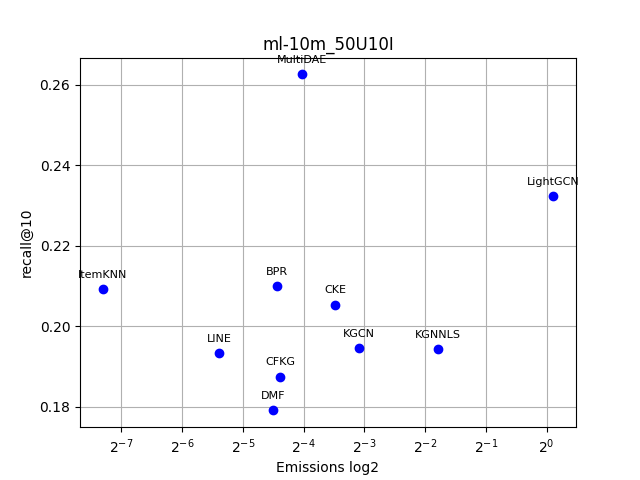
\includegraphics[width=\linewidth, trim=0 0 0 0]{images/recall@10_ml-10m_50U10I.png} &
        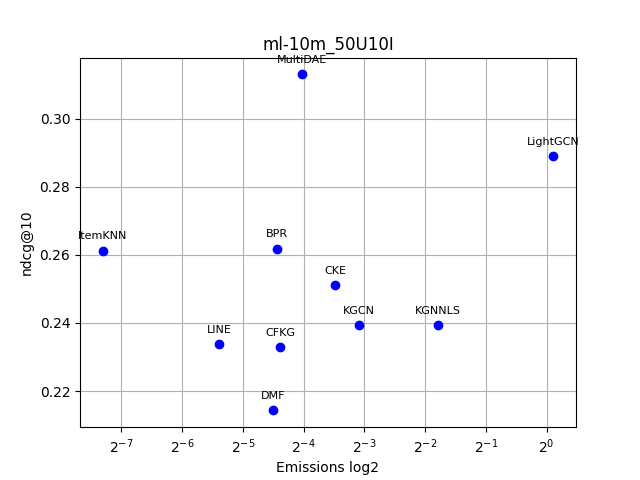
\includegraphics[width=\linewidth, trim=0 0 0 0]{images/ndcg@10_ml-10m_50U10I.png} \\
        \hline
        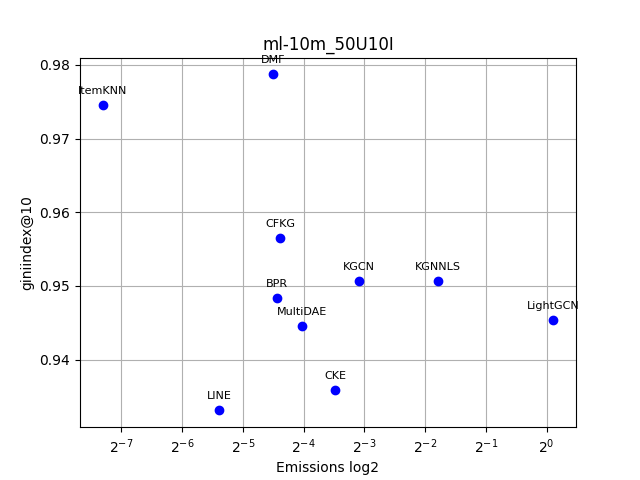
\includegraphics[width=\linewidth, trim=0 0 0 0]{images/giniindex@10_ml-10m_50U10I.png} &
        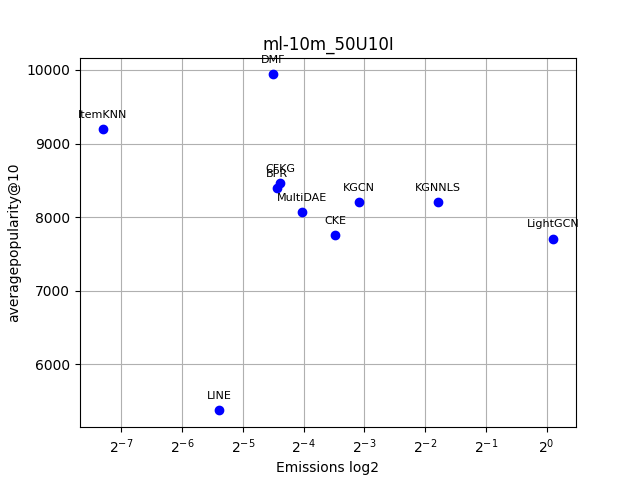
\includegraphics[width=\linewidth, trim=0 0 0 0]{images/averagepopularity@10_ml-10m_50U10I.png} \\
        \hline
    \end{tabularx}
    \caption{Trade-off con il datasetMovieLens-10M\_50U10I}
    \label{tab:emissions_info}
\end{table}


\noindent LightGCN è l'algoritmo che emette di più, osservando i valori da 5 a circa 180 volte rispetto agli altri modelli.
Emissioni cosi alte non sono però giustificate. Nelle metriche di recall e ndcg LightGCN è il secondo migliore, ma la differenza rispetto al primo è molto bassa e quindi non giustifica emissioni così alte.
ItemKNN si conferma uno dei migliori algoritmi per queste due metriche in quanto emette meno ed è uno dei più performanti.
Per quanto riguarda le metriche di Gini Index e Average Popularity possiamo notare che LightGCN è uno di migliori, ma anche in questo caso la differenza rispetto ad altri modelli non giustifica emissioni così alte. ItemKNN si conferma con il secondo peggior modello come punteggi. Line risulta essere il migliore in quanto è il secondo per basse emissioni ed ottiene i punteggi migliori. 


\subsection{Addestramento sostenibile}
\subsubsection{Parte esplorativa}
\paragraph{Primo esperimento} \textcolor{white}{.} \\
\begin{table}[H]
    \centering
    \footnotesize
    \setlength\tabcolsep{0pt}
    \begin{tabularx}{\textwidth}{|X|X|}
        \hline
        \textbf{Criterio classico} & \textbf{Criterio modificato} \\
        \hline
        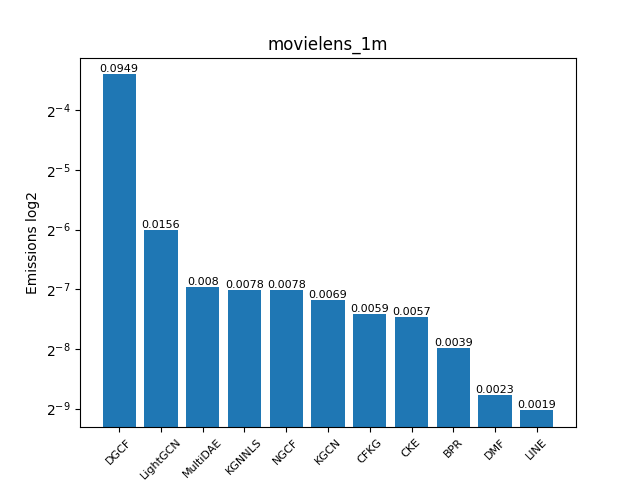
\includegraphics[width=\linewidth, trim=0 0 0 0]{images/emissions_movielens_1m_earlyClassic.png} &
        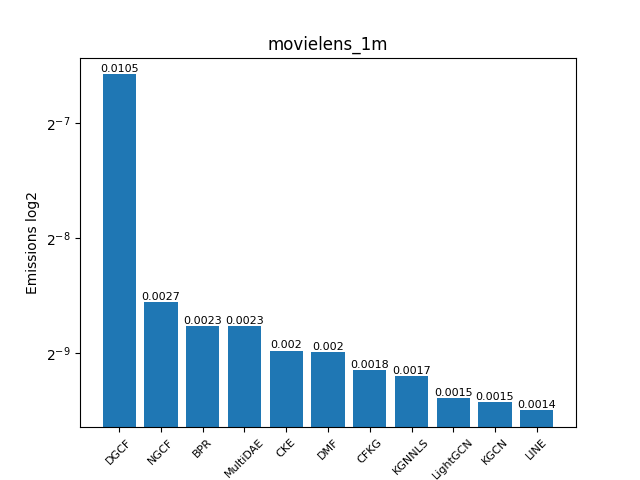
\includegraphics[width=\linewidth, trim=0 0 0 0]{images/emissions_movielens_1m_earlyModified.png} \\
        \hline
    \end{tabularx}
    \caption{Emissioni con criterio classico e modificato}
    \label{tab:emissions_info}
\end{table}

\noindent Si può dunque chiaramente notare come usando il nuovi criterio di early stopping le emissioni siano molto più basse rispetto al criterio classico.

\begin{table}[H]
    \centering
    \resizebox{\textwidth}{!}{
    \begin{tabular}{|c|c|c|c|c|}
        \hline
        \textbf{Modello} & \textbf{Emissioni criterio classico (g)} & \textbf{Emissioni criterio nuovo (g)} & \textbf{Riduzione} & \textbf{\% riduzione emissioni} \\
        \hline
        BPR & 3.9484 & 2.3033 & 1.6451 & 41.6647 \\
        \hline
        CKFG & 5.881 & 1.767 & 4.114 & 69.9418 \\
        \hline
        CKE & 5.68394 & 1.9837 & 3.70024 & 65.09955 \\
        \hline
        DMF & 2.2927 & 1.9667 & 0.326 & 14.2158 \\
        \hline
        KGCN & 6.8754 & 1.454 & 5.4214 & 78.8522 \\
        \hline
        KGNNLS & 7.763 & 1.70177 & 6.0613 & 78.0785 \\
        \hline
        LINE & 1.9128 & 1.3831 & 0.5297 & 27.6935 \\
        \hline
        MultiDAE & 8.0303 & 2.29608 & 5.73422 & 71.40737 \\
        \hline
        LightGCN & 15.626 & 1.4926 & 14.1334 & 90.4481 \\
        \hline
        NGCF & 7.7582 & 2.6601 & 5.0981 & 65.7126 \\
        \hline
        DGCF & 94.903 & 10.4625 & 84.4405 & 88.9756 \\
        \hline
    \end{tabular}
    }
    \caption{Confronto delle emissioni}
\end{table}


\noindent Si può dunque notare come in generale la percentuale di riduzione delle emissioni è molto alta



\begin{figure}[H]
    \centering
    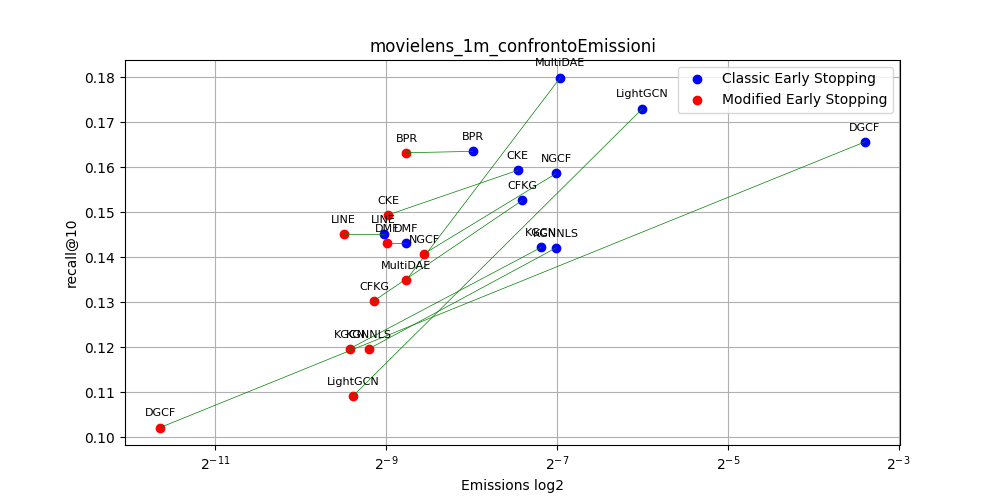
\includegraphics[width=\linewidth, trim=0 0 0 0]{images/recall@10_movielens_1m_comparison.png}
    \caption{Confronto score recall@10 con dataset MovieLens-1m}
    
\end{figure}

\begin{figure}[H]
    \centering
    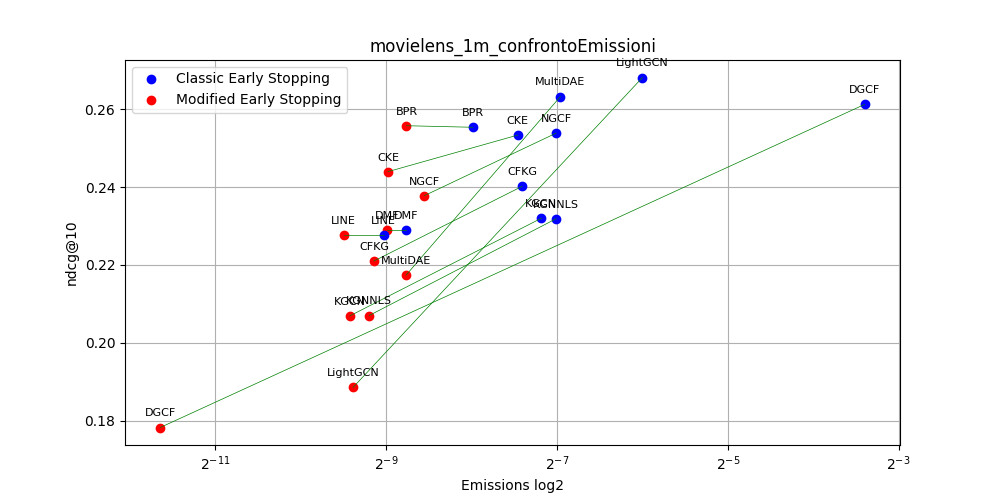
\includegraphics[width=\linewidth, trim=0 0 0 0]{images/ndcg@10_movielens_1m_comparison.png}
    \caption{Confronto score ndcg@10 con dataset MovieLens-1m}
    
\end{figure}

\begin{figure}[H]
    \centering
    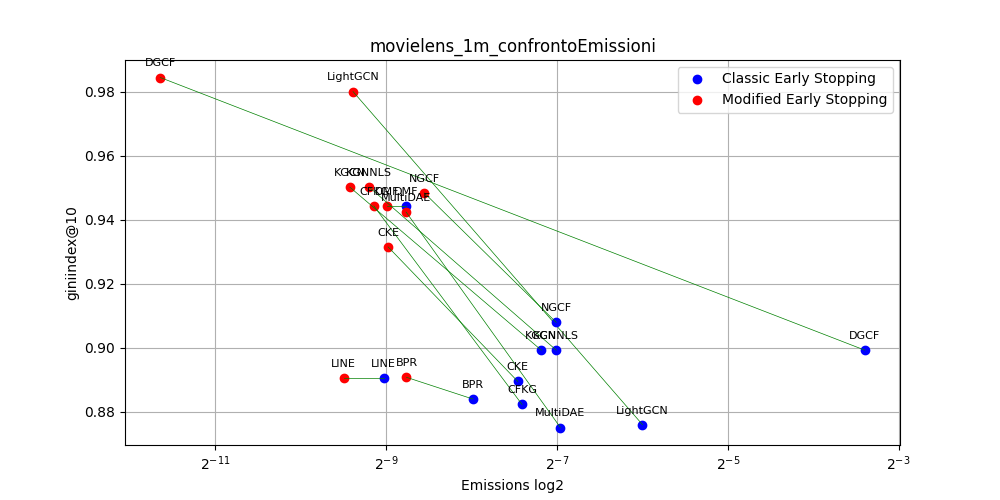
\includegraphics[width=\linewidth, trim=0 0 0 0]{images/giniindex@10_movielens_1m_comparison.png}
    \caption{Confronto score giniindex@10 con dataset MovieLens-1m}
\end{figure}

\begin{figure}[H]
    \centering
    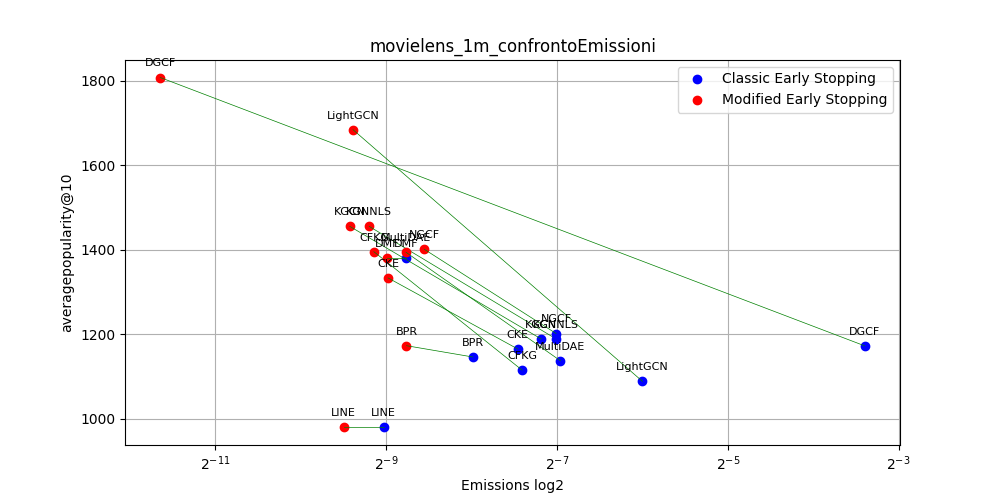
\includegraphics[width=\linewidth, trim=0 0 0 0]{images/averagepopularity@10_movielens_1m_comparison.png}
    \caption{Confronto score averagepopularity@10 con dataset MovieLens-1m}
\end{figure}





\begin{table}[H]
    \centering
    \resizebox{\textwidth}{!}{
        \begin{tabular}{|c|c|c|c|c|c|}
            \hline
            \textbf{Metrica} & \textbf{Modello} & \textbf{Score criterio classico} & \textbf{Score criterio nuovo} & \textbf{Riduzione} & \textbf{\% riduzione score} \\
            \hline
            \multirow{11}{*}{recall@10} & BPR & 0.1635 & 0.1632 & 0.0003 & 0.1835 \\ \cline{2-6}
                                         & CFKG & 0.1526 & 0.1303 & 0.0223 & 14.6134 \\ \cline{2-6}
                                         & CKE & 0.1593 & 0.1494 & 0.0099 & 6.2147 \\ \cline{2-6}
                                         & DMF & 0.1432 & 0.1432 & 0.0 & 0.0 \\ \cline{2-6}
                                         & KGCN & 0.1422 & 0.1197 & 0.0225 & 15.8228 \\ \cline{2-6}
                                         & KGNNLS & 0.1421 & 0.1197 & 0.0224 & 15.7635 \\ \cline{2-6}
                                         & LINE & 0.1451 & 0.1451 & 0.0 & 0.0 \\ \cline{2-6}
                                         & MultiDAE & 0.1799 & 0.1349 & 0.045 & 25.0139 \\ \cline{2-6}
                                         & LightGCN & 0.173 & 0.1092 & 0.0638 & 36.8786 \\ \cline{2-6}
                                         & NGCF & 0.1586 & 0.1408 & 0.0178 & 11.2232 \\ \cline{2-6}
                                         & DGCF & 0.1656 & 0.1022 & 0.0634 & 38.2850 \\ \cline{2-6}
            \hline
            \multirow{11}{*}{ndcg@10} & BPR & 0.2554 & 0.2558 & -0.0004 & -0.1566 \\ \cline{2-6}
                                       & CFKG & 0.2402 & 0.221 & 0.0192 & 7.9933 \\ \cline{2-6}
                                       & CKE & 0.2534 & 0.244 & 0.0094 & 3.7096 \\ \cline{2-6}
                                       & DMF & 0.2289 & 0.2289 & 0.0 & 0.0 \\ \cline{2-6}
                                       & KGCN & 0.232 & 0.2069 & 0.0251 & 10.819 \\ \cline{2-6}
                                       & KGNNLS & 0.2319 & 0.207 & 0.0249 & 10.737 \\ \cline{2-6}
                                       & LINE & 0.2277 & 0.2277 & 0.0 & 0.0 \\ \cline{2-6}
                                       & MultiDAE & 0.2633 & 0.2174 & 0.0459 & 17.433 \\ \cline{2-6}
                                       & LightGCN & 0.2682 & 0.1885 & 0.0797 & 29.717 \\ \cline{2-6}
                                       & NGCF & 0.2539 & 0.2378 & 0.0161 & 6.3411 \\ \cline{2-6}
                                       & DGCF & 0.2613 & 0.1782 & 0.0831 & 31.8025 \\ \cline{2-6}
            \hline
            \multirow{11}{*}{averagepopularity@10} & BPR & 1146.3572 & 1173.1199 & -26.7627 & -2.3346 \\ \cline{2-6}
                                                    & CFKG & 1115.4498 & 1395.6098 & -280.16 & -25.1163 \\ \cline{2-6}
                                                    & CKE & 1165.2413 & 1333.5153 & -168.274 & -14.4411 \\ \cline{2-6}
                                                    & DMF & 1379.7292 & 1379.7292 & 0.0 & 0.0 \\ \cline{2-6}
                                                    & KGCN & 1188.9582 & 1455.5651 & -266.6069 & -22.4236 \\ \cline{2-6}
                                                    & KGNNLS & 1188.8981 & 1455.58 & -266.6819 & -22.4310 \\ \cline{2-6}
                                                    & LINE & 979.498 & 979.498 & 0.0 & 0.0 \\ \cline{2-6}
                                                    & MultiDAE & 1137.4597 & 1394.0944 & -256.6347 & -22.5621 \\ \cline{2-6}
                                                    & LightGCN & 1088.741 & 1684.4149 & -595.6739 & -54.7122 \\ \cline{2-6}
                                                    & NGCF & 1201.8831 & 1401.4325 & -199.5494 & -16.6031 \\ \cline{2-6}
                                                    & DGCF & 1172.6874 & 1807.9828 & -635.2954 & -54.1743 \\ \cline{2-6}
            \hline
            \multirow{11}{*}{giniindex@10} & BPR & 0.8839 & 0.8907 & -0.0068 & -0.7693 \\ \cline{2-6}
                                            & CFKG & 0.8822 & 0.9443 & -0.0621 & -7.0392 \\ \cline{2-6}
                                            & CKE & 0.8894 & 0.9315 & -0.0421 & -4.7335 \\ \cline{2-6}
                                            & DMF & 0.9443 & 0.9443 & 0.0 & 0.0 \\ \cline{2-6}
                                            & KGCN & 0.8992 & 0.9502 & -0.051 & -5.6717 \\ \cline{2-6}
                                            & KGNNLS & 0.8992 & 0.9502 & -0.051 & -5.6717 \\ \cline{2-6}
                                            & LINE & 0.8904 & 0.8904 & 0.0 & 0.0 \\ \cline{2-6}
                                            & MultiDAE & 0.875 & 0.9424 & -0.0674 & -7.7029 \\ \cline{2-6}
                                            & LightGCN & 0.8759 & 0.9801 & -0.1042 & -11.8963 \\ \cline{2-6}
                                            & NGCF & 0.9079 & 0.9484 & -0.0405 & -4.4608 \\     \cline{2-6}
                                            & DGCF & 0.8992 & 0.9845 & -0.0853 & -9.4862 \\ \cline{2-6}
            \hline
        \end{tabular}
    }
    \caption{Confronto degli score tra criteri e modelli}
    \label{tab:confronto-score}
\end{table}


\begin{figure}[H]
    \centering
     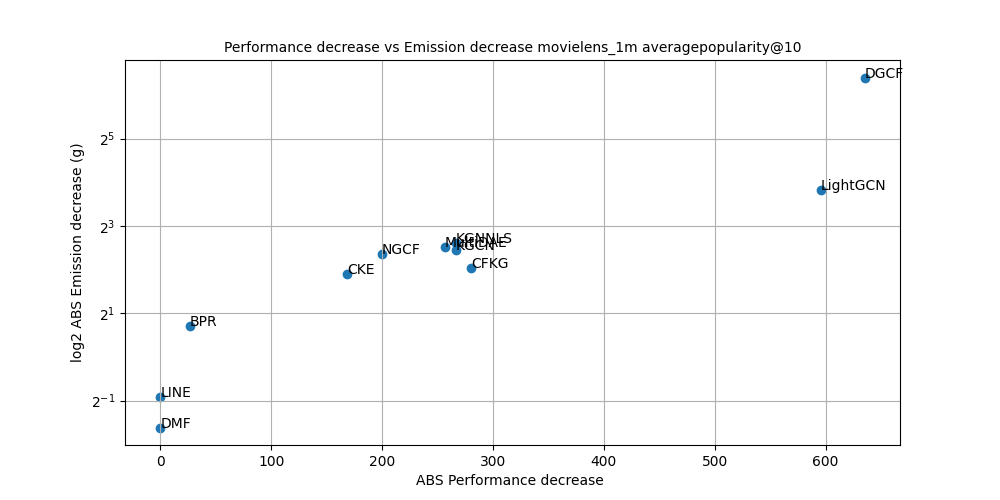
\includegraphics[width=\textwidth]{images/decrement_averagepopularity@10_movielens_1m.png}
    \caption{Decremento di averagepopularity@10}
\end{figure}

\begin{figure}[H]
    \centering
     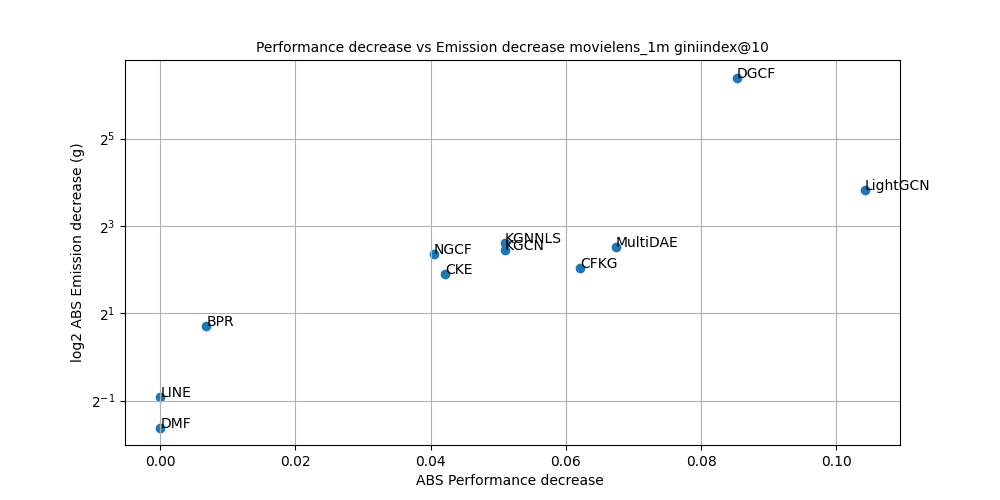
\includegraphics[width=\textwidth]{images/decrement_giniindex@10_movielens_1m.png}
    \caption{Decremento di giniindex@10}
\end{figure}

\begin{figure}[H]
    \centering
     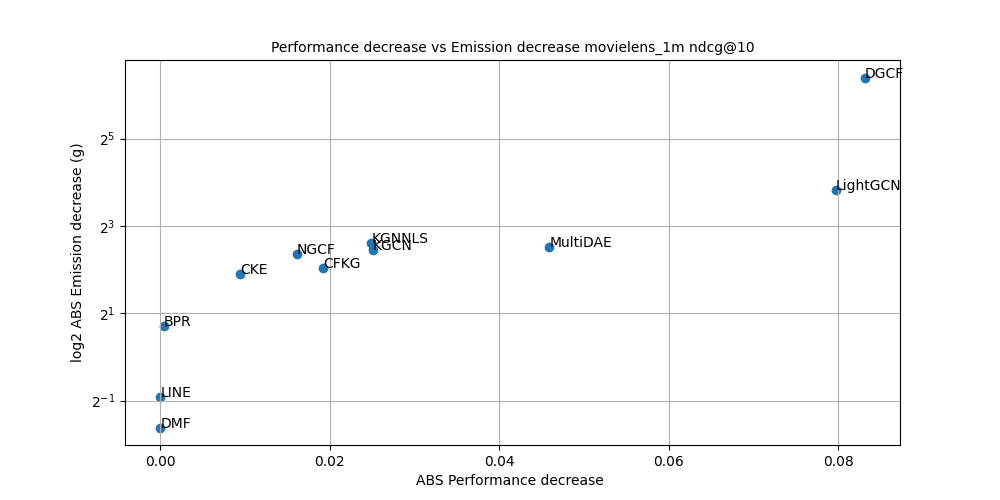
\includegraphics[width=\textwidth]{images/decrement_ndcg@10_movielens_1m.png}
    \caption{Decremento di ndcg@10}
\end{figure}

\begin{figure}[H]
    \centering
     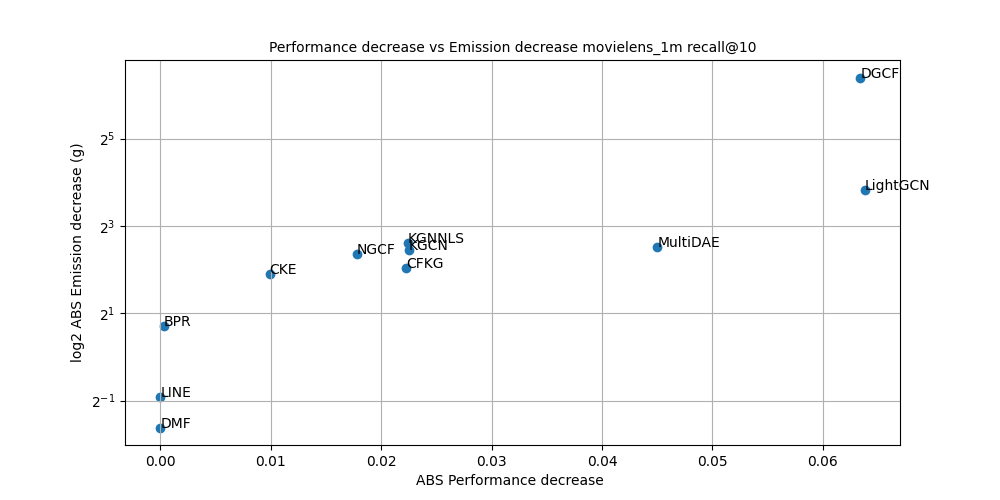
\includegraphics[width=\textwidth]{images/decrement_recall@10_movielens_1m.png}
    \caption{Decremento di recall@10}
\end{figure}


\noindent Per quanto riguarda giniindex e averagepopularity un punteggio più basso è migliore, mentre per recall e ndcg un punteggio più alto è migliore.
Ecco perchè la percentuale di riduzione degli score è negativa per giniindex e averagepopularity.

\noindent Confrontando le percentuali di riduzione delle emissioni e degli score si può notare la riduzione delle emissioni è molto più alta rispetto alla riduzione degli score.

\noindent BPR tende a mantenere le stesse perfomance con entrambi i criteri a fronte di emissioni molto più basse.
Possiamo notare come LINE e DMF non abbiano subito variazioni di score, mentre LightGCN e DGCF abbiano subito una riduzione molto alta (in percentuale comunque molto inferiore rispetto alla riduzione delle emissioni).
Probabilmente per LINE e DMF il criterio di early stopping classico ha portato ad eseguire qualche epoca in più ma che non ha portato a miglioramenti.

\paragraph{Secondo esperimento} \textcolor{white}{.} \\
\begin{table}[H]
    \centering
    \footnotesize
    \setlength\tabcolsep{0pt}
    \begin{tabularx}{\textwidth}{|X|X|}
        \hline
        \textbf{Criterio classico} & \textbf{Criterio modificato} \\
        \hline
        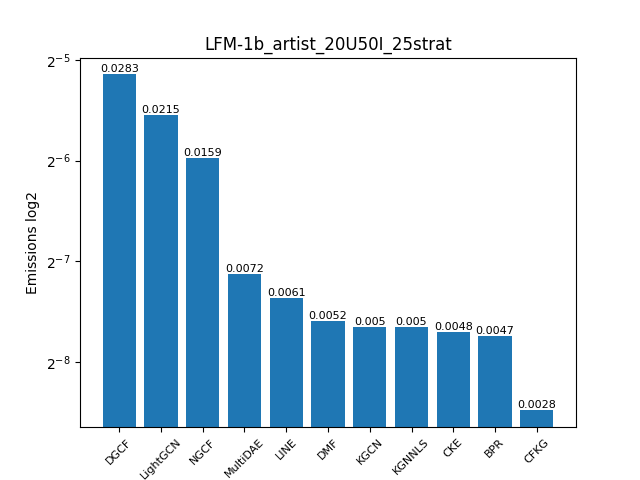
\includegraphics[width=\linewidth, trim=0 0 0 0]{images/emissions_LFM-1b_artist_20U50I_25strat_earlyClassic.png} &
        \includegraphics[width=\linewidth, trim=0 0 0 0]{images/emissions_LFM-1b_artist_20U50I_25strat_earlyModified.png} \\
        \hline
    \end{tabularx}
    \caption{Emissioni con criterio classico e modificato}
    \label{tab:emissions_info}
\end{table}



\begin{table}[H]
    \centering
    \resizebox{\textwidth}{!}{
    \begin{tabular}{|c|c|c|c|c|}
        \hline
        \textbf{Modello} & \textbf{Emissioni criterio classico (g)} & \textbf{Emissioni criterio nuovo (g)} & \textbf{Riduzione} & \textbf{\% riduzione emissioni} \\
        \hline
        BPR & 4.6785 & 4.8381 & -0.1596 & -3.4125 \\
        \hline
        CKFG & 2.8024 & 2.8539 & -0.0515 & -1.8368 \\
        \hline
        CKE & 4.8062 & 1.6694 & 3.1368 & 65.2659 \\
        \hline
        DMF & 5.1886 & 5.3978 & -0.2092 & -4.0321 \\
        \hline
        KGCN & 4.9718 & 5.0108 & -0.039 & -0.7863 \\
        \hline
        KGNNLS & 4.9701 & 5.0453 & -0.0752 & -1.5133 \\
        \hline
        LINE & 6.0602 & 6.2294 & -0.1692 & -2.7912 \\
        \hline
        MultiDAE & 7.1668 & 3.1731 & 3.9937 & 55.7245 \\
        \hline
        LightGCN & 21.4561 & 6.2812 & 15.1749 & 70.7256 \\
        \hline
        NGCF & 15.8887 & 1.0731 & 14.8156 & 93.2463 \\
        \hline
        DGCF & 28.2945 & 5.3468 & 22.9477 & 81.1035 \\
        \hline
    \end{tabular}
    }
    \caption{Confronto delle emissioni}
\end{table}


\noindent Il criterio più stringente mostra chiaramente come la riduzione delle emissioni sia inferiore rispetto al primo esperimento.
Per alcuni modelli vengono registrate addirittura delle variazioni negative, ovvero le emissioni sono aumentate rispetto al criterio classico. Questo potrebbe dipende da un picco di consumi dell'hardware in un certo momento, dovuto a qualche processo in background.
NGCF è l'unico modello in cui si registra un'aumento della percentuale di riduzione delle emissioni rispetto al primo esperimento.


\begin{figure}[H]
    \centering
    \includegraphics[width=\linewidth, trim=0 0 0 0]{images/recall@10_LFM-1b_artist_20U50I_25strat_comparison.png}
    \caption{Confronto score recall@10 con dataset LFM-1b\_artist\_20U50I\_25strat}
    
\end{figure}

\begin{figure}[H]
    \centering
    \includegraphics[width=\linewidth, trim=0 0 0 0]{images/ndcg@10_LFM-1b_artist_20U50I_25strat_comparison.png}
    \caption{Confronto score ndcg@10 con dataset LFM-1b\_artist\_20U50I\_25strat}
    
\end{figure}

\begin{figure}[H]
    \centering
    \includegraphics[width=\linewidth, trim=0 0 0 0]{images/giniindex@10_LFM-1b_artist_20U50I_25strat_comparison.png}
    \caption{Confronto score giniindex@10 con dataset LFM-1b\_artist\_20U50I\_25strat}
\end{figure}

\begin{figure}[H]
    \centering
    \includegraphics[width=\linewidth, trim=0 0 0 0]{images/averagepopularity@10_LFM-1b_artist_20U50I_25strat_comparison.png}
    \caption{Confronto score averagepopularity@10 con dataset LFM-1b\_artist\_20U50I\_25strat}
\end{figure}


\begin{table}[H]
    \centering
    \resizebox{\textwidth}{!}{
        \begin{tabular}{|c|c|c|c|c|c|}
            \hline
            \textbf{Metrica} & \textbf{Modello} & \textbf{Score criterio classico} & \textbf{Score criterio nuovo} & \textbf{Riduzione} & \textbf{\% riduzione score} \\
            \hline
            \multirow{11}{*}{recall@10} & BPR & 0.0772 & 0.0772 & 0.0 & 0.0 \\ \cline{2-6}
                                        & CFKG & 0.1387 & 0.1387 & 0.0 & 0.0 \\ \cline{2-6}
                                        & CKE & 0.1078 & 0.1066 & -0.0121 & -1.1257 \\ \cline{2-6}
                                        & DMF & 0.0698 & 0.0698 & 0.0 & 0.0 \\ \cline{2-6}
                                        & KGCN & 0.1299 & 0.1299 & 0.0 & 0.0 \\ \cline{2-6}
                                        & KGNNLS & 0.1299 & 0.1299 & 0.0 & 0.0 \\ \cline{2-6}
                                        & LINE & 0.0496 & 0.0496 & 0.0 & 0.0 \\ \cline{2-6}
                                        & MultiDAE & 0.0806 & 0.1024 & 0.0218 & 21.2891 \\ \cline{2-6}
                                        & LightGCN & 0.0773 & 0.1012 & 0.0239 & 23.6166 \\ \cline{2-6}
                                        & NGCF & 0.0183 & 0.0947 & 0.0764 & 80.6758 \\\cline{2-6}
                                        & DGCF & 0.0774 & 0.0901 & 0.0127 & 14.0954 \\ \cline{2-6}
            \hline
            \multirow{11}{*}{ndcg@10} & BPR & 0.04 & 0.04 & 0.0 & 0.0 \\ \cline{2-6}
                                      & CFKG & 0.0687 & 0.0687 & 0.0 & 0.0 \\ \cline{2-6}
                                      & CKE & 0.0532 & 0.0539 & 0.0007 & 1.2987 \\ \cline{2-6}
                                      & DMF & 0.0359 & 0.0359 & 0.0 & 0.0 \\ \cline{2-6}
                                      & KGCN & 0.0621 & 0.0621 & 0.0 & 0.0 \\ \cline{2-6}
                                      & KGNNLS & 0.0621 & 0.0621 & 0.0 & 0.0 \\ \cline{2-6}
                                      & LINE & 0.0261 & 0.0261 & 0.0 & 0.0 \\ \cline{2-6}
                                      & MultiDAE & 0.0419 & 0.0522 & 0.0103 & 19.7318 \\ \cline{2-6}
                                      & LightGCN & 0.0399 & 0.0523 & 0.0124 & 23.7094 \\ \cline{2-6}
                                      & NGCF & 0.009 & 0.0488 & 0.0398 & 81.5574 \\ \cline{2-6}
                                      & DGCF & 0.0397 & 0.0464 & 0.0067 & 14.4397 \\ \cline{2-6}
            \hline
            \multirow{11}{*}{averagepopularity@10} & BPR & 877.7191 & 877.7191 & 0.0 & 0.0 \\ \cline{2-6}
                                                  & CFKG & 686.1384 & 686.1384 & 0.0 & 0.0 \\ \cline{2-6}
                                                  & CKE & 507.6022 & 492.1156 & -15.4866 & -3.1469 \\ \cline{2-6}
                                                  & DMF & 872.5193 & 872.5193 & 0.0 & 0.0 \\ \cline{2-6}
                                                  & KGCN & 635.7879 & 635.7879 & 0.0 & 0.0 \\ \cline{2-6}
                                                  & KGNNLS & 635.7866 & 635.7866 & 0.0 & 0.0 \\\cline{2-6}
                                                  & LINE & 244.7699 & 244.7699 & 0.0 & 0.0 \\ \cline{2-6}
                                                  & MultiDAE & 929.5664 & 700.0905 & -229.4759 & -32.778 \\ \cline{2-6}
                                                  & LightGCN & 902.6965 & 680.2857 & -222.4108 & -32.6937 \\ \cline{2-6}
                                                  & NGCF & 112.7163 & 734.8359 & 622.1196 & 84.661 \\ \cline{2-6}
                                                  & DGCF & 892.5034 & 742.4452 & -150.0582 & -20.2114 \\ \cline{2-6}
            \hline
            \multirow{11}{*}{giniindex@10} & BPR & 0.9991 & 0.9991 & 0.0 & 0.0 \\ \cline{2-6}
                                            & CFKG & 0.9989 & 0.9989 & 0.0 & 0.0 \\ \cline{2-6}
                                            & CKE & 0.9929 & 0.9926 & -0.0003 & -0.0302 \\ \cline{2-6}
                                            & DMF & 0.9996 & 0.9996 & 0.0 & 0.0 \\ \cline{2-6}
                                            & KGCN & 0.9978 & 0.9978 & 0.0 & 0.0 \\ \cline{2-6}
                                            & KGNNLS & 0.9978 & 0.9978 & 0.0 & 0.0 \\ \cline{2-6}
                                            & LINE & 0.984 & 0.984 & 0.0 & 0.0 \\ \cline{2-6}
                                            & MultiDAE & 0.9995 & 0.998 & -0.0015 & -0.1503 \\ \cline{2-6}
                                            & LightGCN & 0.9993 & 0.9953 & -0.004 & -0.4019 \\ \cline{2-6}
                                            & NGCF & 0.8987 & 0.9865 & 0.0878 & 8.9002 \\ \cline{2-6}
                                            & DGCF & 0.9993 & 0.996 & -0.0033 & -0.3313 \\ \cline{2-6}
            \hline
        \end{tabular}
    }
    \caption{Confronto degli score tra criteri e modelli}
\end{table}




\begin{figure}[H]
    \centering
     \includegraphics[width=\textwidth]{images/decrement_averagepopularity@10_LFM-1b_artist_20U50I_25strat.png}
    \caption{Decremento di averagepopularity@10}
\end{figure}

\begin{figure}[H]
    \centering
     \includegraphics[width=\textwidth]{images/decrement_giniindex@10_LFM-1b_artist_20U50I_25strat.png}
    \caption{Decremento di giniindex@10}
\end{figure}

\begin{figure}[H]
    \centering
     \includegraphics[width=\textwidth]{images/decrement_ndcg@10_LFM-1b_artist_20U50I_25strat.png}
    \caption{Decremento di ndcg@10}
\end{figure}

\begin{figure}[H]
    \centering
     \includegraphics[width=\textwidth]{images/decrement_recall@10_LFM-1b_artist_20U50I_25strat.png}
    \caption{Decremento di recall@10}
\end{figure}


\noindent Si può chiaramente notare come gli algoritmi che prima avevano registrato un aumento delle emissioni abbiano le stesse performance ad ogni metrica.
Questo è un chiaro segno che in questo caso gli algoritmi in entrambi i casi abbiano terminato l'esecuzione con il criterio di early stopping classico e che le emissioni abbiano subito un picco in un certo momento dovuto ad altri fattori.
Si può chiaramente notare come, rispetto al primo esperimento, tutti gli altri modelli, ad eccezione di NGCF, abbiano subito una riduzione delle performance molto più bassa rispetto al primo esperimento a fronte di riduzione di emissioni minori, a conferma che il criterio più stringente ha permesso a questi modelli di continuare l'addestramento e dunque essere allenati per più epoche.
Un anomalia si può notare per NGCF, che ha subito una riduzione delle performance molto alta rispetto al primo esperimento a fronte di una riduzione delle emissioni molto più alte. In entrambi i casi la differenza di errore è dell'ordine dei centesimi. Questo potrebbe essere dovuto al un dataset con diverse caratteristiche rispetto al precedente.

\paragraph{Terzo esperimento} \textcolor{white}{.} \\
\begin{table}[H]
    \centering
    \footnotesize
    \setlength\tabcolsep{0pt}
    \begin{tabularx}{\textwidth}{|X|X|}
        \hline
        \textbf{Criterio classico} & \textbf{Criterio modificato} \\
        \hline
        \includegraphics[width=\linewidth, trim=0 0 0 0]{images/emissions_amazon_books_60core_kg_earlyClassic.png} &
        \includegraphics[width=\linewidth, trim=0 0 0 0]{images/emissions_amazon_books_60core_kg_earlyModified.png} \\
        \hline
    \end{tabularx}
    \caption{Emissioni con criterio classico e modificato}
    \label{tab:emissions_info}
\end{table}



\begin{table}[H]
    \centering
    \resizebox{\textwidth}{!}{
    \begin{tabular}{|c|c|c|c|c|}
        \hline
        \textbf{Modello} & \textbf{Emissioni criterio classico (g)} & \textbf{Emissioni criterio nuovo (g)} & \textbf{Riduzione} & \textbf{\% riduzione emissioni}\\
        \hline
        BPR & 34.3235 & 3.2958 & 31.0277 & 90.398\\
        \hline
        CKFG & 53.7798 & 2.4515 & 51.3283 & 95.4416\\
        \hline
        CKE & 21.1537 & 1.5824 & 19.5713 & 92.5194\\
        \hline
        DMF & 22.9403 & 8.8401 & 14.1002 & 61.4649\\
        \hline
        KGCN & 45.1294 & 2.7897 & 42.3397 & 93.8185\\
        \hline
        KGNNLS & 40.1533 & 2.8432 & 37.3101 & 92.9192\\
        \hline
        LINE & 32.5426 & 3.2539 & 29.2887 & 90.0011\\
        \hline
        MultiDAE & 30.3706 & 3.2749 & 27.0957 & 89.2169\\
        \hline
        LightGCN & 91.732 & 4.3526 & 87.3794 & 95.2551\\
        \hline
        NGCF & 49.55 & 4.0757 & 45.4743 & 91.7745\\
        \hline
    \end{tabular}
    }
    \caption{Confronto delle emissioni}
\end{table}

\noindent Come è possibile notare in questo caso la riduzione delle emissioni è molto alta per tutti i modelli, con valori che superano il 90\% per quasi tutti i modelli.


\begin{figure}[H]
    \centering
    \includegraphics[width=\linewidth, trim=0 0 0 0]{images/recall@10_amazon_books_60core_kg_comparison.png}
    \caption{Confronto score recall@10 con dataset amazon\_books\_60core\_kg}
    
\end{figure}

\begin{figure}[H]
    \centering
    \includegraphics[width=\linewidth, trim=0 0 0 0]{images/ndcg@10_amazon_books_60core_kg_comparison.png}
    \caption{Confronto score ndcg@10 con dataset amazon\_books\_60core\_kg}
    
\end{figure}

\begin{figure}[H]
    \centering
    \includegraphics[width=\linewidth, trim=0 0 0 0]{images/giniindex@10_amazon_books_60core_kg_comparison.png}
    \caption{Confronto score giniindex@10 con dataset amazon\_books\_60core\_kg}
\end{figure}

\begin{figure}[H]
    \centering
    \includegraphics[width=\linewidth, trim=0 0 0 0]{images/averagepopularity@10_amazon_books_60core_kg_comparison.png}
    \caption{Confronto score averagepopularity@10 con dataset amazon\_books\_60core\_kg}
\end{figure}


\begin{table}[H]
    \centering
    \resizebox{\textwidth}{!}{
    \begin{tabular}{|c|c|c|c|c|c|}
        \hline
        \textbf{Metrica} & \textbf{Modello} & \textbf{Score criterio classico} & \textbf{Score criterio nuovo} & \textbf{Riduzione} & \textbf{\% riduzione score} \\ \hline
        \multirow{11}{*}{recall@10} & BPR & 0.0393 & 0.0214 & 0.0179 & 45.5471 \\ \cline{2-6} 
                                     & CFKG & 0.0929 & 0.0243 & 0.0686 & 73.8428 \\ \cline{2-6} 
                                     & CKE & 0.0977 & 0.0532 & 0.0445 & 45.5476 \\ \cline{2-6} 
                                     & DMF & 0.0216 & 0.021 & 0.0006 & 2.7778 \\ \cline{2-6} 
                                     & KGCN & 0.0644 & 0.0334 & 0.031 & 48.1366 \\ \cline{2-6} 
                                     & KGNNLS & 0.0625 & 0.0333 & 0.0292 & 46.72 \\ \cline{2-6} 
                                     & LINE & 0.0391 & 0.0192 & 0.0199 & 50.8951 \\ \cline{2-6} 
                                     & MultiDAE & 0.0609 & 0.0206 & 0.0403 & 66.1741 \\ \cline{2-6} 
                                     & LightGCN & 0.0526 & 0.0196 & 0.033 & 62.7376 \\ \cline{2-6} 
                                     & NGCF & 0.0374 & 0.017 & 0.0204 & 54.5455 \\ \cline{2-6} 
        \hline
        \multirow{11}{*}{ndcg@10} & BPR & 0.0357 & 0.0202 & 0.0155 & 43.4174 \\ \cline{2-6} 
                                   & CFKG & 0.0556 & 0.0135 & 0.0421 & 75.7194 \\ \cline{2-6} 
                                   & CKE & 0.0585 & 0.0309 & 0.0276 & 47.1795 \\ \cline{2-6} 
                                   & DMF & 0.0208 & 0.0199 & 0.0009 & 4.3269 \\ \cline{2-6} 
                                   & KGCN & 0.0373 & 0.0189 & 0.0184 & 49.3298 \\ \cline{2-6} 
                                   & KGNNLS & 0.0363 & 0.0188 & 0.0175 & 48.2094 \\ \cline{2-6} 
                                   & LINE & 0.0342 & 0.0189 & 0.0153 & 44.7368 \\ \cline{2-6} 
                                   & MultiDAE & 0.0543 & 0.0192 & 0.0351 & 64.6409 \\ \cline{2-6} 
                                   & LightGCN & 0.0472 & 0.0185 & 0.0287 & 60.8051 \\ \cline{2-6} 
                                   & NGCF & 0.0339 & 0.0166 & 0.0173 & 51.0324 \\ \cline{2-6} 
        \hline
        \multirow{11}{*}{avgpopularity@10} & BPR & 109.4148 & 220.0387 & -110.6239 & -101.1051 \\ \cline{2-6} 
                                            & CFKG & 122.3777 & 366.0359 & -243.6582 & -199.1034 \\ \cline{2-6} 
                                            & CKE & 117.927 & 229.8594 & -111.9324 & -94.9167 \\ \cline{2-6} 
                                            & DMF & 158.1008 & 156.3042 & 1.7966 & 1.1364 \\ \cline{2-6} 
                                            & KGCN & 140.0346 & 256.0119 & -115.9773 & -82.8205 \\ \cline{2-6} 
                                            & KGNNLS & 147.1768 & 256.0278 & -108.851 & -73.9593 \\ \cline{2-6} 
                                            & LINE & 58.1057 & 100.9865 & -42.8808 & -73.7979 \\ \cline{2-6} 
                                            & MultiDAE & 76.5618 & 207.1265 & -130.5647 & -170.535 \\ \cline{2-6} 
                                            & LightGCN & 105.7397 & 252.0464 & -146.3067 & -138.365 \\ \cline{2-6} 
                                            & NGCF & 113.2036 & 70.9028 & 42.3008 & 37.367 \\ \cline{2-6} 
        \hline
        \multirow{11}{*}{giniindex@10} & BPR & 0.9007 & 0.9926 & -0.0919 & -10.2032 \\ \cline{2-6} 
                                        & CFKG & 0.8093 & 0.9981 & -0.1888 & -23.3288 \\ \cline{2-6} 
                                        & CKE & 0.8287 & 0.9862 & -0.1575 & -19.0057 \\ \cline{2-6} 
                                        & DMF & 0.9858 & 0.9875 & -0.0017 & -0.1724 \\ \cline{2-6} 
                                        & KGCN & 0.8637 & 0.9892 & -0.1255 & -14.5305 \\ \cline{2-6} 
                                        & KGNNLS & 0.8828 & 0.9892 & -0.1064 & -12.0526 \\ \cline{2-6} 
                                        & LINE & 0.7542 & 0.9807 & -0.2265 & -30.0318 \\ \cline{2-6} 
                                        & MultiDAE & 0.7543 & 0.9938 & -0.2395 & -31.7513 \\ \cline{2-6} 
                                        & LightGCN & 0.8761 & 0.9964 & -0.1203 & -13.7313 \\ \cline{2-6} 
                                        & NGCF & 0.9011 & 0.7956 & 0.1055 & 11.7079 \\ \cline{2-6} 
        \hline
    \end{tabular}
    }
    \caption{Performance dei modelli su diverse metriche e dataset}
\end{table}


\begin{figure}[H]
    \centering
     \includegraphics[width=\textwidth]{images/decrement_averagepopularity@10_amazon_books_60core_kg.png}
    \caption{Decremento di averagepopularity@10}
\end{figure}

\begin{figure}[H]
    \centering
     \includegraphics[width=\textwidth]{images/decrement_giniindex@10_amazon_books_60core_kg.png}
    \caption{Decremento di giniindex@10}
\end{figure}

\begin{figure}[H]
    \centering
     \includegraphics[width=\textwidth]{images/decrement_ndcg@10_amazon_books_60core_kg.png}
    \caption{Decremento di ndcg@10}
\end{figure}

\begin{figure}[H]
    \centering
     \includegraphics[width=\textwidth]{images/decrement_recall@10_amazon_books_60core_kg.png}
    \caption{Decremento di recall@10}
\end{figure}
\noindent Si può notare come le forti riduzioni di emissioni abbiano portato a una riduzione delle performance molto più alta rispetto ai due esperimenti precedenti.
DMF è l'unico modello che ha mantenuto performance quasi invarianti a fronte di una riduzione delle emissioni del 61\%. (la più bassa ma comunque molto alta).




\subsubsection{Confronto tra i criteri}

\paragraph{Primo esperimento} \textcolor{white}{.} \\
\begin{table}[H]
    \centering
    \footnotesize
    \setlength\tabcolsep{0pt}
    \begin{tabularx}{\textwidth}{|X|X|}
        \hline
        \textbf{Criterio classico} & \textbf{Criterio modificato} \\
        \hline
        \includegraphics[width=\linewidth, trim=0 0 0 0]{images/emissions_movielens_1m_40_5_earlyClassic.png} &
        \includegraphics[width=\linewidth, trim=0 0 0 0]{images/emissions_movielens_1m_40_5_earlyModified.png} \\
        \hline
    \end{tabularx}
    \caption{Emissioni con criterio classico e modificato}
    \label{tab:emissions_info}
\end{table}




\begin{table}[H]
    \centering
    \resizebox{\textwidth}{!}{
    \begin{tabular}{|c|c|c|c|c|}
        \hline
        \textbf{Modello} & \textbf{Emissioni criterio classico (g)} & \textbf{Emissioni criterio nuovo (g)} & \textbf{Riduzione} & \textbf{\% riduzione emissioni} \\
        \hline
        BPR & 3.9484 & 2.2898 & 1.6586 & 42.0068 \\
        \hline
        CKFG & 5.881 & 1.7411 & 4.1399 & 70.3944 \\
        \hline
        CKE & 5.6839 & 2.0271 & 3.6568 & 64.3357 \\
        \hline
        DMF & 2.2927 & 1.9885 & 0.3042 & 13.2688 \\
        \hline
        KGCN & 6.8754 & 3.8305 & 3.0449 & 44.2875 \\
        \hline
        KGNNLS & 7.763 & 1.7384 & 6.0246 & 77.607 \\
        \hline
        LINE & 1.9129 & 1.4341 & 0.4788 & 25.0296 \\
        \hline
        MultiDAE & 8.0303 & 2.9614 & 5.0689 & 63.68 \\
        \hline
        LightGCN & 15.626 & 1.6634 & 13.9626 & 89.3547 \\
        \hline
        NGCF & 7.7582 & 2.7574 & 5.0008 & 64.4576 \\
        \hline
        DGCF & 94.903 & 10.4183 & 84.4847 & 89.0222 \\
        \hline

    \end{tabular}
    }
    \caption{Confronto delle emissioni}
\end{table}

\noindent Possiamo notare un'elevata riduzione delle emissioni per quasi tutti i modelli.

\begin{figure}[H]
    \centering
    \includegraphics[width=\linewidth, trim=0 0 0 0]{images/recall@10_movielens_1m_40_5_comparison.png}
    \caption{Confronto score recall@10}
    
\end{figure}

\begin{figure}[H]
    \centering
    \includegraphics[width=\linewidth, trim=0 0 0 0]{images/ndcg@10_movielens_1m_40_5_comparison.png}
    \caption{Confronto score ndcg@10}
    
\end{figure}

\begin{figure}[H]
    \centering
    \includegraphics[width=\linewidth, trim=0 0 0 0]{images/giniindex@10_movielens_1m_40_5_comparison.png}
    \caption{Confronto score giniindex@10}
\end{figure}

\begin{figure}[H]
    \centering
    \includegraphics[width=\linewidth, trim=0 0 0 0]{images/averagepopularity@10_movielens_1m_40_5_comparison.png}
    \caption{Confronto score averagepopularity@10}
\end{figure}

\begin{table}[H]
    \centering
    \resizebox{\textwidth}{!}{
    \begin{tabular}{|c|c|c|c|c|c|}
        \hline
        \textbf{Metrica} & \textbf{Modello} & \textbf{Score criterio classico} & \textbf{Score criterio nuovo} & \textbf{Riduzione} & \textbf{\% riduzione score} \\ \hline
        \multirow{11}{*}{recall@10} 
            & BPR & 0.1635 & 0.1632 & 0.0003 & 0.1835 \\ \cline{2-6} 
            & CFKG & 0.1526 & 0.1303 & 0.0223 & 14.6134 \\ \cline{2-6} 
            & CKE & 0.1593 & 0.1494 & 0.0099 & 6.2147 \\ \cline{2-6} 
            & DMF & 0.1432 & 0.1432 & 0.0 & 0.0 \\ \cline{2-6} 
            & KGCN & 0.1422 & 0.1422 & 0.0 & 0.0 \\ \cline{2-6} 
            & KGNNLS & 0.1421 & 0.1197 & 0.0224 & 15.7635 \\ \cline{2-6} 
            & LINE & 0.1451 & 0.1451 & 0.0 & 0.0 \\ \cline{2-6} 
            & MultiDAE & 0.1799 & 0.1489 & 0.031 & 17.2318 \\ \cline{2-6} 
            & LightGCN & 0.173 & 0.1111 & 0.0619 & 35.7803 \\ \cline{2-6} 
            & NGCF & 0.1586 & 0.1408 & 0.0178 & 11.2232 \\ \cline{2-6} 
            & DGCF & 0.1656 & 0.1022 & 0.0634 & 38.285 \\ \hline

        \multirow{11}{*}{ndcg@10} 
            & BPR & 0.2554 & 0.2558 & -0.0004 & -0.1566 \\ \cline{2-6} 
            & CFKG & 0.2402 & 0.221 & 0.0192 & 7.9933 \\ \cline{2-6} 
            & CKE & 0.2534 & 0.244 & 0.0094 & 3.7096 \\ \cline{2-6} 
            & DMF & 0.2289 & 0.2289 & 0.0 & 0.0 \\ \cline{2-6} 
            & KGCN & 0.232 & 0.2333 & -0.0013 & -0.5603 \\ \cline{2-6} 
            & KGNNLS & 0.2319 & 0.207 & 0.0249 & 10.7374 \\ \cline{2-6} 
            & LINE & 0.2277 & 0.2277 & 0.0 & 0.0 \\ \cline{2-6} 
            & MultiDAE & 0.2633 & 0.2336 & 0.0297 & 11.2799 \\ \cline{2-6} 
            & LightGCN & 0.2682 & 0.1924 & 0.0758 & 28.2625 \\ \cline{2-6} 
            & NGCF & 0.2539 & 0.2378 & 0.0161 & 6.3411 \\ \cline{2-6} 
            & DGCF & 0.2613 & 0.1782 & 0.0831 & 31.8025 \\ \hline

        \multirow{11}{*}{avgpopularity@10} 
            & BPR & 1146.3572 & 1173.1199 & -26.7627 & -2.3346 \\ \cline{2-6} 
            & CFKG & 1115.4498 & 1395.6098 & -280.16 & -25.1163 \\ \cline{2-6} 
            & CKE & 1165.2413 & 1333.5153 & -168.274 & -14.4411 \\ \cline{2-6} 
            & DMF & 1379.7292 & 1379.7292 & 0.0 & 0.0 \\ \cline{2-6} 
            & KGCN & 1188.9582 & 1193.5298 & -4.5716 & -0.3845 \\ \cline{2-6} 
            & KGNNLS & 1188.8981 & 1455.58 & -266.6819 & -22.431 \\ \cline{2-6} 
            & LINE & 979.498 & 979.498 & 0.0 & 0.0 \\ \cline{2-6} 
            & MultiDAE & 1137.4597 & 1335.1498 & -197.69 & -17.38 \\ \cline{2-6} 
            & LightGCN & 1088.741 & 1662.4263 & -573.6853 & -52.6925 \\ \cline{2-6} 
            & NGCF & 1201.8831 & 1401.4325 & -199.5494 & -16.6031 \\ \cline{2-6} 
            & DGCF & 1172.6874 & 1807.8717 & -635.1843 & -54.1648 \\ \hline

        \multirow{11}{*}{giniindex@10} 
            & BPR & 0.8839 & 0.8907 & -0.0068 & -0.7693 \\ \cline{2-6} 
            & CFKG & 0.8822 & 0.9443 & -0.0621 & -7.0392 \\ \cline{2-6} 
            & CKE & 0.8894 & 0.9315 & -0.0421 & -4.7335 \\ \cline{2-6} 
            & DMF & 0.9443 & 0.9443 & 0.0 & 0.0 \\ \cline{2-6} 
            & KGCN & 0.8992 & 0.9012 & -0.002 & -0.2224 \\ \cline{2-6} 
            & KGNNLS & 0.8992 & 0.9502 & -0.051 & -5.6717 \\ \cline{2-6} 
            & LINE & 0.8904 & 0.8904 & 0.0 & 0.0 \\ \cline{2-6} 
            & MultiDAE & 0.875 & 0.9283 & -0.0533 & -6.0914 \\ \cline{2-6} 
            & LightGCN & 0.8759 & 0.9783 & -0.1024 & -11.6908 \\ \cline{2-6} 
            & NGCF & 0.9079 & 0.9484 & -0.0405 & -4.4608 \\ \cline{2-6} 
            & DGCF & 0.8992 & 0.9845 & -0.0853 & -9.4862 \\ \hline
    \end{tabular}
    }
    \caption{Performance dei modelli su diverse metriche e dataset}
\end{table}

\begin{figure}[H]
    \centering
     \includegraphics[width=\textwidth]{images/decrement_averagepopularity@10_movielens_1m_40_5.png}
    \caption{Decremento di averagepopularity@10}
\end{figure}

\begin{figure}[H]
    \centering
     \includegraphics[width=\textwidth]{images/decrement_giniindex@10_movielens_1m_40_5.png}
    \caption{Decremento di giniindex@10}
\end{figure}

\begin{figure}[H]
    \centering
     \includegraphics[width=\textwidth]{images/decrement_ndcg@10_movielens_1m_40_5.png}
    \caption{Decremento di ndcg@10}
\end{figure}

\begin{figure}[H]
    \centering
     \includegraphics[width=\textwidth]{images/decrement_recall@10_movielens_1m_40_5.png}
    \caption{Decremento di recall@10}
\end{figure}
\noindent Il calo delle performance abbastanza contenuto rispetto alla riduzione delle emissioni, con un decremento di averagepopularity@10 molto alto per alcuni modelli (LightGCN e DGCF in particolare).

\paragraph{Secondo esperimento} \textcolor{white}{.} \\
\begin{table}[H]
    \centering
    \footnotesize
    \setlength\tabcolsep{0pt}
    \begin{tabularx}{\textwidth}{|X|X|}
        \hline
        \textbf{Criterio classico} & \textbf{Criterio modificato} \\
        \hline
        \includegraphics[width=\linewidth, trim=0 0 0 0]{images/emissions_movielens_1m_30_5_earlyClassic.png} &
        \includegraphics[width=\linewidth, trim=0 0 0 0]{images/emissions_movielens_1m_30_5_earlyModified.png} \\
        \hline
    \end{tabularx}
    \caption{Emissioni con criterio classico e modificato}
    \label{tab:emissions_info}
\end{table}



\begin{table}[H]
    \centering
    \resizebox{\textwidth}{!}{
    \begin{tabular}{|c|c|c|c|c|}
        \hline
        \textbf{Modello} & \textbf{Emissioni criterio classico (g)} & \textbf{Emissioni criterio nuovo (g)} & \textbf{Riduzione} & \textbf{\% riduzione emissioni}\\
        \hline
        BPR & 3.9484 & 2.5219 & 1.4265 & 36.1284 \\ \hline
        CKFG & 5.881 & 1.8872 & 3.9938 & 67.9104 \\ \hline
        CKE & 5.6839 & 2.0466 & 3.6373 & 63.9932 \\ \hline
        DMF & 2.2927 & 2.0856 & 0.2071 & 9.0319 \\ \hline
        KGCN & 6.8754 & 3.796 & 3.0794 & 44.7884 \\ \hline
        KGNNLS & 7.763 & 4.3657 & 3.3973 & 43.7626 \\ \hline
        LINE & 1.9129 & 1.4314 & 0.4815 & 25.1721 \\ \hline
        MultiDAE & 8.0303 & 3.9614 & 4.0689 & 50.4865 \\ \hline
        LightGCN & 15.626 & 1.9001 & 13.7259 & 87.8402 \\ \hline
        NGCF & 7.7582 & 2.6923 & 5.0659 & 65.2979 \\ \hline
        DGCF & 94.903 & 10.4109 & 84.4921 & 89.03 \\ \hline
    \end{tabular}
    }
    \caption{Confronto delle emissioni}
\end{table}

\noindent Rispetto al primo esperimento si può facilemnte notare come una soglia più bassa abbia portato a un generale diminuzione della percentuale di riduzione delle emissioni (cioè gli algoritmi hanno eseguito un training più lungo).


\begin{figure}[H]
    \centering
    \includegraphics[width=\linewidth, trim=0 0 0 0]{images/recall@10_movielens_1m_30_5_comparison.png}
    \caption{Confronto score recall@10}
    
\end{figure}

\begin{figure}[H]
    \centering
    \includegraphics[width=\linewidth, trim=0 0 0 0]{images/ndcg@10_movielens_1m_30_5_comparison.png}
    \caption{Confronto score ndcg@10}
    
\end{figure}

\begin{figure}[H]
    \centering
    \includegraphics[width=\linewidth, trim=0 0 0 0]{images/giniindex@10_movielens_1m_30_5_comparison.png}
    \caption{Confronto score giniindex@10}
\end{figure}

\begin{figure}[H]
    \centering
    \includegraphics[width=\linewidth, trim=0 0 0 0]{images/averagepopularity@10_movielens_1m_30_5_comparison.png}
    \caption{Confronto score averagepopularity@10}
\end{figure}


\begin{table}[H]
    \centering
    \resizebox{\textwidth}{!}{
    \begin{tabular}{|c|c|c|c|c|c|}
        \hline
        \textbf{Metrica} & \textbf{Modello} & \textbf{Score criterio classico} & \textbf{Score criterio nuovo} & \textbf{Riduzione} & \textbf{\% riduzione score} \\ \hline
        \multirow{11}{*}{recall@10} 
            & BPR & 0.1635 & 0.1635 & 0.0 & 0.0 \\ \cline{2-6} 
            & CFKG & 0.1526 & 0.1301 & 0.0225 & 14.7444 \\ \cline{2-6} 
            & CKE & 0.1593 & 0.1494 & 0.0099 & 6.2147 \\ \cline{2-6} 
            & DMF & 0.1432 & 0.1432 & 0.0 & 0.0 \\ \cline{2-6} 
            & KGCN & 0.1422 & 0.1422 & 0.0 & 0.0 \\ \cline{2-6} 
            & KGNNLS & 0.1421 & 0.1423 & -0.0002 & -0.1407 \\ \cline{2-6} 
            & LINE & 0.1451 & 0.1451 & 0.0 & 0.0 \\ \cline{2-6} 
            & MultiDAE & 0.1799 & 0.1619 & 0.018 & 10.0056 \\ \cline{2-6} 
            & LightGCN & 0.173 & 0.1161 & 0.0569 & 32.8902 \\ \cline{2-6} 
            & NGCF & 0.1586 & 0.1408 & 0.0178 & 11.2232 \\ \cline{2-6} 
            & DGCF & 0.1656 & 0.1021 & 0.0635 & 38.3454 \\ \hline

        \multirow{11}{*}{ndcg@10} 
            & BPR & 0.2554 & 0.2554 & 0.0 & 0.0 \\ \cline{2-6} 
            & CFKG & 0.2402 & 0.2209 & 0.0193 & 8.035 \\ \cline{2-6} 
            & CKE & 0.2534 & 0.244 & 0.0094 & 3.7096 \\ \cline{2-6} 
            & DMF & 0.2289 & 0.2289 & 0.0 & 0.0 \\ \cline{2-6} 
            & KGCN & 0.232 & 0.2333 & -0.0013 & -0.5603 \\ \cline{2-6} 
            & KGNNLS & 0.2319 & 0.2334 & -0.0015 & -0.6468 \\ \cline{2-6} 
            & LINE & 0.2277 & 0.2277 & 0.0 & 0.0 \\ \cline{2-6} 
            & MultiDAE & 0.2633 & 0.247 & 0.0163 & 6.1907 \\ \cline{2-6} 
            & LightGCN & 0.2682 & 0.2002 & 0.068 & 25.3542 \\ \cline{2-6} 
            & NGCF & 0.2539 & 0.2378 & 0.0161 & 6.3411 \\ \cline{2-6} 
            & DGCF & 0.2613 & 0.1781 & 0.0832 & 31.8408 \\ \hline

        \multirow{11}{*}{avgpopularity@10} 
            & BPR & 1146.3572 & 1146.3572 & 0.0 & 0.0 \\ \cline{2-6} 
            & CFKG & 1115.4498 & 1361.1447 & -245.6949 & -22.0265 \\ \cline{2-6} 
            & CKE & 1165.2413 & 1333.5153 & -168.274 & -14.4411 \\ \cline{2-6} 
            & DMF & 1379.7292 & 1379.7292 & 0.0 & 0.0 \\ \cline{2-6} 
            & KGCN & 1188.9582 & 1193.5298 & -4.5716 & -0.3845 \\ \cline{2-6} 
            & KGNNLS & 1188.8981 & 1193.7263 & -4.8282 & -0.4061 \\ \cline{2-6} 
            & LINE & 979.498 & 979.498 & 0.0 & 0.0 \\ \cline{2-6} 
            & MultiDAE & 1137.4597 & 1261.7868 & -124.3271 & -10.9302 \\ \cline{2-6} 
            & LightGCN & 1088.741 & 1629.6349 & -540.8939 & -49.6807 \\ \cline{2-6} 
            & NGCF & 1201.8831 & 1401.4325 & -199.5494 & -16.6031 \\ \cline{2-6} 
            & DGCF & 1172.6874 & 1807.9008 & -635.2134 & -54.1673 \\ \hline

        \multirow{11}{*}{giniindex@10} 
            & BPR & 0.8839 & 0.8839 & 0.0 & 0.0 \\ \cline{2-6} 
            & CFKG & 0.8822 & 0.9401 & -0.0579 & -6.5631 \\ \cline{2-6} 
            & CKE & 0.8894 & 0.9315 & -0.0421 & -4.7335 \\ \cline{2-6} 
            & DMF & 0.9443 & 0.9443 & 0.0 & 0.0 \\ \cline{2-6} 
            & KGCN & 0.8992 & 0.9012 & -0.002 & -0.2224 \\ \cline{2-6} 
            & KGNNLS & 0.8992 & 0.9013 & -0.0021 & -0.2335 \\ \cline{2-6} 
            & LINE & 0.8904 & 0.8904 & 0.0 & 0.0 \\ \cline{2-6} 
            & MultiDAE & 0.875 & 0.9101 & -0.0351 & -4.0114 \\ \cline{2-6} 
            & LightGCN & 0.8759 & 0.9748 & -0.0989 & -11.2912 \\ \cline{2-6} 
            & NGCF & 0.9079 & 0.9484 & -0.0405 & -4.4608 \\ \cline{2-6} 
            & DGCF & 0.8992 & 0.9845 & -0.0853 & -9.4862 \\ \hline
    \end{tabular}
    }
    \caption{Performance dei modelli su diverse metriche e dataset}
\end{table}


\begin{figure}[H]
    \centering
     \includegraphics[width=\textwidth]{images/decrement_averagepopularity@10_movielens_1m_30_5.png}
    \caption{Decremento di averagepopularity@10}
\end{figure}

\begin{figure}[H]
    \centering
     \includegraphics[width=\textwidth]{images/decrement_giniindex@10_movielens_1m_30_5.png}
    \caption{Decremento di giniindex@10}
\end{figure}

\begin{figure}[H]
    \centering
     \includegraphics[width=\textwidth]{images/decrement_ndcg@10_movielens_1m_30_5.png}
    \caption{Decremento di ndcg@10}
\end{figure}

\begin{figure}[H]
    \centering
     \includegraphics[width=\textwidth]{images/decrement_recall@10_movielens_1m_30_5.png}
    \caption{Decremento di recall@10}
\end{figure}
\noindent Rispetto allo scorso esperimento, KGNNLS escluso, tutti i modelli hanno avuto un comportamento pressochè simile all'esperimento precedente emettendo leggermente di più. Dunque la combinazione di parametri 40 e 5 si è rivelata migliore di 30 e 5

\paragraph{Terzo esperimento} \textcolor{white}{.} \\
\begin{table}[H]
    \centering
    \footnotesize
    \setlength\tabcolsep{0pt}
    \begin{tabularx}{\textwidth}{|X|X|}
        \hline
        \textbf{Criterio classico} & \textbf{Criterio modificato} \\
        \hline
        \includegraphics[width=\linewidth, trim=0 0 0 0]{images/emissions_movielens_1m_40_6_earlyClassic.png} &
        \includegraphics[width=\linewidth, trim=0 0 0 0]{images/emissions_movielens_1m_40_6_earlyModified.png} \\
        \hline
    \end{tabularx}
    \caption{Emissioni con criterio classico e modificato}
    \label{tab:emissions_info}
\end{table}




\begin{table}[H]
    \centering
    \resizebox{\textwidth}{!}{
    \begin{tabular}{|c|c|c|c|c|}
        \hline
        \textbf{Modello} & \textbf{Emissioni criterio classico (g)} & \textbf{Emissioni criterio nuovo (g)} & \textbf{Riduzione} & \textbf{\% riduzione emissioni}\\
        \hline
        BPR & 3.9484 & 2.483 & 1.4654 & 37.1154\\ \hline
        CKFG & 5.881 & 1.8037 & 4.0773 & 69.3305\\ \hline
        CKE & 5.6839 & 2.0806 & 3.6033 & 63.3944\\ \hline
        DMF & 2.2927 & 2.9977 & 0.2949 & 12.869\\ \hline
        KGCN & 6.8754 & 3.9708 & 2.9046 & 42.2461\\ \hline
        KGNNLS & 7.763 & 1.8709 & 5.8921 & 75.8996\\ \hline
        LINE & 1.9129 & 1.396 & 0.5169 & 27.0205\\ \hline
        MultiDAE & 8.0303 & 3.048 & 4.9823 & 62.044\\ \hline
        LightGCN & 15.626 & 1.7426 & 13.8834 & 88.8482\\ \hline
        NGCF & 7.7582 & 2.821 & 4.9372 & 63.6387\\ \hline
        DGCF & 94.903 & 11.8866 & 83.0164 & 87.475\\ \hline
    \end{tabular}
    }
    \caption{Confronto delle emissioni }
\end{table}

\noindent Rispetto al primo esperimento la percentuale di riduzioni delle emissioni in generale è diminuita. Rispetto al secondo esperimento, invece, la percentuale di riduzione delle emissioni è diminuita per alcuni modelli e aumentata per altri.


\begin{figure}[H]
    \centering
    \includegraphics[width=\linewidth, trim=0 0 0 0]{images/recall@10_movielens_1m_40_6_comparison.png}
    \caption{Confronto score recall@10}
    
\end{figure}

\begin{figure}[H]
    \centering
    \includegraphics[width=\linewidth, trim=0 0 0 0]{images/ndcg@10_movielens_1m_40_6_comparison.png}
    \caption{Confronto score ndcg@10}
    
\end{figure}

\begin{figure}[H]
    \centering
    \includegraphics[width=\linewidth, trim=0 0 0 0]{images/giniindex@10_movielens_1m_40_6_comparison.png}
    \caption{Confronto score giniindex@10}
\end{figure}

\begin{figure}[H]
    \centering
    \includegraphics[width=\linewidth, trim=0 0 0 0]{images/averagepopularity@10_movielens_1m_40_6_comparison.png}
    \caption{Confronto score averagepopularity@10}
\end{figure}


\begin{table}[H]
    \centering
    \resizebox{\textwidth}{!}{
        \begin{tabular}{|c|c|c|c|c|c|}
            \hline
            \textbf{Metrica} & \textbf{Modello} & \textbf{Score criterio classico} & \textbf{Score criterio nuovo} & \textbf{Riduzione} & \textbf{\% riduzione score} \\ \hline
            \multirow{11}{*}{recall@10} 
                & BPR & 0.1635 & 0.1635 & 0.0 & 0.0 \\ \cline{2-6} 
                & CFKG & 0.1526 & 0.1301 & 0.0225 & 14.7444 \\ \cline{2-6} 
                & CKE & 0.1593 & 0.1517 & 0.0076 & 4.7709 \\ \cline{2-6} 
                & DMF & 0.1432 & 0.1432 & 0.0 & 0.0 \\ \cline{2-6} 
                & KGCN & 0.1422 & 0.1422 & 0.0 & 0.0 \\ \cline{2-6} 
                & KGNNLS & 0.1421 & 0.1232 & 0.0189 & 13.3005 \\ \cline{2-6} 
                & LINE & 0.1451 & 0.1451 & 0.0 & 0.0 \\ \cline{2-6} 
                & MultiDAE & 0.1799 & 0.1531 & 0.0268 & 14.8972 \\ \cline{2-6} 
                & LightGCN & 0.173 & 0.1126 & 0.0604 & 34.9133 \\ \cline{2-6} 
                & NGCF & 0.1586 & 0.1438 & 0.0148 & 9.3317 \\ \cline{2-6} 
                & DGCF & 0.1656 & 0.108 & 0.0576 & 34.7826 \\ \hline

            \multirow{11}{*}{ndcg@10} 
                & BPR & 0.2554 & 0.2554 & 0.0 & 0.0 \\ \cline{2-6} 
                & CFKG & 0.2402 & 0.2209 & 0.0193 & 8.035 \\ \cline{2-6} 
                & CKE & 0.2534 & 0.2482 & 0.0052 & 2.0521 \\ \cline{2-6} 
                & DMF & 0.2289 & 0.2289 & 0.0 & 0.0 \\ \cline{2-6} 
                & KGCN & 0.232 & 0.2328 & -0.0008 & -0.3448 \\ \cline{2-6} 
                & KGNNLS & 0.2319 & 0.2115 & 0.0204 & 8.7969 \\ \cline{2-6} 
                & LINE & 0.2277 & 0.2277 & 0.0 & 0.0 \\ \cline{2-6} 
                & MultiDAE & 0.2633 & 0.2372 & 0.0261 & 9.9126 \\ \cline{2-6} 
                & LightGCN & 0.2682 & 0.1955 & 0.0727 & 27.1066 \\ \cline{2-6} 
                & NGCF & 0.2539 & 0.2401 & 0.0138 & 5.4352 \\ \cline{2-6} 
                & DGCF & 0.2613 & 0.1857 & 0.0756 & 28.9323 \\ \hline

            \multirow{11}{*}{averagepopularity@10} 
                & BPR & 1146.3572 & 1146.3572 & 0.0 & 0.0 \\ \cline{2-6} 
                & CFKG & 1115.4498 & 1361.1447 & -245.6949 & -22.0265 \\ \cline{2-6} 
                & CKE & 1165.2413 & 1320.1912 & -154.9499 & -13.2977 \\ \cline{2-6} 
                & DMF & 1379.7292 & 1379.7292 & 0.0 & 0.0 \\ \cline{2-6} 
                & KGCN & 1188.9582 & 1187.2098 & 1.7484 & 0.1471 \\ \cline{2-6} 
                & KGNNLS & 1188.8981 & 1401.0945 & -212.1964 & -17.8482 \\ \cline{2-6} 
                & LINE & 979.498 & 979.498 & 0.0 & 0.0 \\ \cline{2-6} 
                & MultiDAE & 1137.4597 & 1297.2825 & -159.8228 & -14.0509 \\ \cline{2-6} 
                & LightGCN & 1088.741 & 1649.9548 & -561.2138 & -51.547 \\ \cline{2-6} 
                & NGCF & 1201.8831 & 1407.3654 & -205.4823 & -17.0967 \\ \cline{2-6} 
                & DGCF & 1172.6874 & 1760.7243 & -588.0369 & -50.1444 \\ \hline

            \multirow{11}{*}{giniindex@10} 
                & BPR & 0.8839 & 0.8839 & 0.0 & 0.0 \\ \cline{2-6} 
                & CFKG & 0.8822 & 0.9401 & -0.0579 & -6.5631 \\ \cline{2-6} 
                & CKE & 0.8894 & 0.9266 & -0.0372 & -4.1826 \\ \cline{2-6} 
                & DMF & 0.9443 & 0.9443 & 0.0 & 0.0 \\ \cline{2-6} 
                & KGCN & 0.8992 & 0.8984 & 0.0008 & 0.089 \\ \cline{2-6} 
                & KGNNLS & 0.8992 & 0.945 & -0.0458 & -5.0934 \\ \cline{2-6} 
                & LINE & 0.8904 & 0.8904 & 0.0 & 0.0 \\ \cline{2-6} 
                & MultiDAE & 0.875 & 0.9204 & -0.0454 & -5.1886 \\ \cline{2-6} 
                & LightGCN & 0.8759 & 0.9767 & -0.1008 & -11.5082 \\ \cline{2-6} 
                & NGCF & 0.9079 & 0.9481 & -0.0402 & -4.4278 \\ \cline{2-6} 
                & DGCF & 0.8992 & 0.982 & -0.0828 & -9.2082 \\ \hline
        \end{tabular}
    }
    \caption{Performance dei modelli su diverse metriche e dataset}
\end{table}



\begin{figure}[H]
    \centering
     \includegraphics[width=\textwidth]{images/decrement_averagepopularity@10_movielens_1m_40_6.png}
    \caption{Decremento di averagepopularity@10}
\end{figure}

\begin{figure}[H]
    \centering
     \includegraphics[width=\textwidth]{images/decrement_giniindex@10_movielens_1m_40_6.png}
    \caption{Decremento di giniindex@10}
\end{figure}

\begin{figure}[H]
    \centering
     \includegraphics[width=\textwidth]{images/decrement_ndcg@10_movielens_1m_40_6.png}
    \caption{Decremento di ndcg@10}
\end{figure}

\begin{figure}[H]
    \centering
     \includegraphics[width=\textwidth]{images/decrement_recall@10_movielens_1m_40_6.png}
    \caption{Decremento di recall@10}
\end{figure}

\noindent Rispetto al primo esperimento la riduzione delle performance sono diminuite (cioè gli algoritmi hanno performato meglio). Anche rispetto al secondo esperimento (con alcune eccezzioni come KGNNLS) le performance sono più alte, anche se di poco.

\paragraph{Quarto esperimento} \textcolor{white}{.} \\
\begin{table}[H]
    \centering
    \footnotesize
    \setlength\tabcolsep{0pt}
    \begin{tabularx}{\textwidth}{|X|X|}
        \hline
        \textbf{Criterio classico} & \textbf{Criterio modificato} \\
        \hline
        \includegraphics[width=\linewidth, trim=0 0 0 0]{images/emissions_movielens_1m_30_6_earlyClassic.png} &
        \includegraphics[width=\linewidth, trim=0 0 0 0]{images/emissions_movielens_1m_30_6_earlyModified.png} \\
        \hline
    \end{tabularx}
    \caption{Emissioni con criterio classico e modificato}
    \label{tab:emissions_info}
\end{table}



\begin{table}[H]
    \centering
    \resizebox{\textwidth}{!}{
    \begin{tabular}{|c|c|c|c|c|}
        \hline
        \textbf{Modello} & \textbf{Emissioni criterio classico (g)} & \textbf{Emissioni criterio nuovo (g)} & \textbf{Riduzione} & \textbf{\% riduzione emissioni}\\
        \hline
        BPR & 3.9484 & 3.1221 & 0.8263 & 20.93\\ \hline
        CFKG & 5.881 & 1.9202 & 3.9608 & 67.35\\ \hline
        CKE & 5.6839 & 2.078 & 3.6059 & 63.44\\ \hline
        DMF & 2.2927 & 1.9962 & 0.2965 & 12.93\\ \hline
        KGCN & 6.8754 & 3.9292 & 2.9462 & 42.85\\ \hline
        KGNNLS & 7.763 & 4.7984 & 2.9646 & 38.19\\ \hline
        LINE & 1.9129 & 1.3937 & 0.5192 & 27.14\\ \hline
        MultiDAE & 8.0303 & 3.7405 & 4.2898 & 53.42\\ \hline
        LightGCN & 15.626 & 2.1161 & 13.5099 & 86.46\\ \hline
        NGCF & 7.7582 & 2.885 & 4.8732 & 62.81\\ \hline
        DGCF & 94.903 & 12.0604 & 82.8426 & 87.2918\\ \hline
    \end{tabular}
    }
    \caption{Confronto delle emissioni }
\end{table}


\noindent Rispetto a tutti e tre gli esperimenti precedenti la percentuale di riduzioni delle emissioni in generale è diminuita, dunque gli algoritmi hanno emesso di più.


\begin{figure}[H]
    \centering
    \includegraphics[width=\linewidth, trim=0 0 0 0]{images/recall@10_movielens_1m_30_6_comparison.png}
    \caption{Confronto score recall@10}
    
\end{figure}

\begin{figure}[H]
    \centering
    \includegraphics[width=\linewidth, trim=0 0 0 0]{images/ndcg@10_movielens_1m_30_6_comparison.png}
    \caption{Confronto score ndcg@10}
    
\end{figure}

\begin{figure}[H]
    \centering
    \includegraphics[width=\linewidth, trim=0 0 0 0]{images/giniindex@10_movielens_1m_30_6_comparison.png}
    \caption{Confronto score giniindex@10}
\end{figure}

\begin{figure}[H]
    \centering
    \includegraphics[width=\linewidth, trim=0 0 0 0]{images/averagepopularity@10_movielens_1m_30_6_comparison.png}
    \caption{Confronto score averagepopularity@10}
\end{figure}


\begin{table}[H]
    \centering
    \resizebox{\textwidth}{!}{
        \begin{tabular}{|c|c|c|c|c|c|}
            \hline
            \textbf{Metrica} & \textbf{Modello} & \textbf{Score criterio classico} & \textbf{Score criterio nuovo} & \textbf{Riduzione} & \textbf{\% riduzione score} \\ \hline
            \multirow{11}{*}{recall@10} 
                & BPR & 0.1635 & 0.1635 & 0.0 & 0.0 \\ \cline{2-6} 
                & CFKG & 0.1526 & 0.1344 & 0.0182 & 11.9266 \\ \cline{2-6} 
                & CKE & 0.1593 & 0.1517 & 0.0076 & 4.7709 \\ \cline{2-6} 
                & DMF & 0.1432 & 0.1432 & 0.0 & 0.0 \\ \cline{2-6} 
                & KGCN & 0.1422 & 0.1422 & 0.0 & 0.0 \\ \cline{2-6} 
                & KGNNLS & 0.1421 & 0.1421 & 0.0 & 0.0 \\ \cline{2-6} 
                & LINE & 0.1451 & 0.1451 & 0.0 & 0.0 \\ \cline{2-6} 
                & MultiDAE & 0.1799 & 0.1624 & 0.0175 & 9.7276 \\ \cline{2-6} 
                & LightGCN & 0.173 & 0.1204 & 0.0526 & 30.4046 \\ \cline{2-6} 
                & NGCF & 0.1586 & 0.1438 & 0.0148 & 9.3317 \\ \cline{2-6} 
                & DGCF & 0.1656 & 0.108 & 0.0576 & 34.7826 \\ \hline

            \multirow{11}{*}{ndcg@10} 
                & BPR & 0.2554 & 0.2554 & 0.0 & 0.0 \\ \cline{2-6} 
                & CFKG & 0.2402 & 0.2245 & 0.0157 & 6.5362 \\ \cline{2-6} 
                & CKE & 0.2534 & 0.2482 & 0.0052 & 2.0521 \\ \cline{2-6} 
                & DMF & 0.2289 & 0.2289 & 0.0 & 0.0 \\ \cline{2-6} 
                & KGCN & 0.232 & 0.2328 & -0.0008 & -0.3448 \\ \cline{2-6} 
                & KGNNLS & 0.2319 & 0.2327 & -0.0008 & -0.345 \\ \cline{2-6} 
                & LINE & 0.2277 & 0.2277 & 0.0 & 0.0 \\ \cline{2-6} 
                & MultiDAE & 0.2633 & 0.2463 & 0.017 & 6.4565 \\ \cline{2-6} 
                & LightGCN & 0.2682 & 0.2064 & 0.0618 & 23.0425 \\ \cline{2-6} 
                & NGCF & 0.2539 & 0.2401 & 0.0138 & 5.4352 \\ \cline{2-6} 
                & DGCF & 0.2613 & 0.1857 & 0.0756 & 28.9323 \\ \hline

            \multirow{11}{*}{averagepopularity@10} 
                & BPR & 1146.3572 & 1146.3572 & 0.0 & 0.0 \\ \cline{2-6} 
                & CFKG & 1115.4498 & 1338.642 & -223.1922 & -20.0092 \\ \cline{2-6} 
                & CKE & 1165.2413 & 1320.1912 & -154.9499 & -13.2977 \\ \cline{2-6} 
                & DMF & 1379.7292 & 1379.7292 & 0.0 & 0.0 \\ \cline{2-6} 
                & KGCN & 1188.9582 & 1187.2098 & 1.7484 & 0.1471 \\ \cline{2-6} 
                & KGNNLS & 1188.8981 & 1187.2158 & 1.6823 & 0.1415 \\ \cline{2-6} 
                & LINE & 979.498 & 979.498 & 0.0 & 0.0 \\ \cline{2-6} 
                & MultiDAE & 1137.4597 & 1238.6498 & -101.1901 & -8.8961 \\ \cline{2-6} 
                & LightGCN & 1088.741 & 1585.7381 & -496.9971 & -45.6488 \\ \cline{2-6} 
                & NGCF & 1201.8831 & 1407.3654 & -205.4823 & -17.0967 \\ \cline{2-6} 
                & DGCF & 1172.6874 & 1760.6621 & -587.9747 & -50.1391 \\ \hline

            \multirow{11}{*}{giniindex@10} 
                & BPR & 0.8839 & 0.8839 & 0.0 & 0.0 \\ \cline{2-6} 
                & CFKG & 0.8822 & 0.9367 & -0.0545 & -6.1777 \\ \cline{2-6} 
                & CKE & 0.8894 & 0.9266 & -0.0372 & -4.1826 \\ \cline{2-6} 
                & DMF & 0.9443 & 0.9443 & 0.0 & 0.0 \\ \cline{2-6} 
                & KGCN & 0.8992 & 0.8984 & 0.0008 & 0.089 \\ \cline{2-6} 
                & KGNNLS & 0.8992 & 0.8983 & 0.0009 & 0.1001 \\ \cline{2-6} 
                & LINE & 0.8904 & 0.8904 & 0.0 & 0.0 \\ \cline{2-6} 
                & MultiDAE & 0.875 & 0.9054 & -0.0304 & -3.4743 \\ \cline{2-6} 
                & LightGCN & 0.8759 & 0.9709 & -0.095 & -10.846 \\ \cline{2-6} 
                & NGCF & 0.9079 & 0.9481 & -0.0402 & -4.4278 \\ \cline{2-6} 
                & DGCF & 0.8992 & 0.982 & -0.0828 & -9.2082 \\ \hline
        \end{tabular}
    }
    \caption{Performance dei modelli su diverse metriche e dataset}
\end{table}



\begin{figure}[H]
    \centering
     \includegraphics[width=\textwidth]{images/decrement_averagepopularity@10_movielens_1m_30_6.png}
    \caption{Decremento di averagepopularity@10}
\end{figure}

\begin{figure}[H]
    \centering
     \includegraphics[width=\textwidth]{images/decrement_giniindex@10_movielens_1m_30_6.png}
    \caption{Decremento di giniindex@10}
\end{figure}

\begin{figure}[H]
    \centering
     \includegraphics[width=\textwidth]{images/decrement_ndcg@10_movielens_1m_30_6.png}
    \caption{Decremento di ndcg@10}
\end{figure}

\begin{figure}[H]
    \centering
     \includegraphics[width=\textwidth]{images/decrement_recall@10_movielens_1m_30_6.png}
    \caption{Decremento di recall@10}
\end{figure}

\noindent Rispetto ai 3 esperimenti la percentuale di riduzione delle performance è diminuita. Per ora dunque questo è l'esperimento che ha emesso di più e performato.

\paragraph{Quinto esperimento} \textcolor{white}{.} \\ 
\begin{table}[H]
    \centering
    \footnotesize
    \setlength\tabcolsep{0pt}
    \begin{tabularx}{\textwidth}{|X|X|}
        \hline
        \textbf{Criterio classico} & \textbf{Criterio modificato} \\
        \hline
        \includegraphics[width=\linewidth, trim=0 0 0 0]{images/emissions_movielens_1m_40_7_earlyClassic.png} &
        \includegraphics[width=\linewidth, trim=0 0 0 0]{images/emissions_movielens_1m_40_7_earlyModified.png} \\
        \hline
    \end{tabularx}
    \caption{Emissioni con criterio classico e modificato}
    \label{tab:emissions_info}
\end{table}



\begin{table}[H]
    \centering
    \resizebox{\textwidth}{!}{
    \begin{tabular}{|c|c|c|c|c|}
        \hline
        \textbf{Modello} & \textbf{Emissioni criterio classico (g)} & \textbf{Emissioni criterio nuovo (g)} & \textbf{Riduzione} & \textbf{\% riduzione emissioni} \\
        \hline
        BPR & 3.9484 & 3.2382 & 0.7102 & 17.9867 \\ \hline
        CFKG & 5.881 & 1.9178 & 3.9632 & 67.3907 \\ \hline
        CKE & 5.6839 & 2.32 & 3.3639 & 59.1839 \\ \hline
        DMF & 2.2927 & 1.9929 & 0.2998 & 13.0788 \\ \hline
        KGCN & 6.8754 & 4.0376 & 2.8378 & 41.2747 \\ \hline
        KGNNLS & 7.763 & 2.0222 & 5.7408 & 73.9507 \\ \hline
        LINE & 1.9129 & 1.3883 & 0.5246 & 27.4219 \\ \hline
        MultiDAE & 8.0303 & 3.1853 & 4.845 & 60.3338 \\ \hline
        LightGCN & 15.626 & 1.8528 & 13.7732 & 88.1427 \\ \hline
        NGCF & 7.7582 & 3.1472 & 4.611 & 59.4342 \\ \hline
        DGCF & 94.903 & 13.3956 & 81.5074 & 85.885 \\ \hline
    \end{tabular}
    }
    \caption{Confronto delle emissioni }
\end{table}


\noindent Rispetto al quarto esperimento la percentuale di riduzioni delle emissioni in generale è diminuita, dunque gli algoritmi hanno emesso di più.
Ci sono poche eccezioni che potrebbero essere dovute alla presenza di processi in background sulla macchina che hanno portato a un consumo leggermente più elevato dell'hardware.


\begin{figure}[H]
    \centering
    \includegraphics[width=\linewidth, trim=0 0 0 0]{images/recall@10_movielens_1m_40_7_comparison.png}
    \caption{Confronto score recall@10}
    
\end{figure}

\begin{figure}[H]
    \centering
    \includegraphics[width=\linewidth, trim=0 0 0 0]{images/ndcg@10_movielens_1m_40_7_comparison.png}
    \caption{Confronto score ndcg@10}
    
\end{figure}

\begin{figure}[H]
    \centering
    \includegraphics[width=\linewidth, trim=0 0 0 0]{images/giniindex@10_movielens_1m_40_7_comparison.png}
    \caption{Confronto score giniindex@10}
\end{figure}

\begin{figure}[H]
    \centering
    \includegraphics[width=\linewidth, trim=0 0 0 0]{images/averagepopularity@10_movielens_1m_40_7_comparison.png}
    \caption{Confronto score averagepopularity@10}
\end{figure}


\begin{table}[H]
    \centering
    \resizebox{\textwidth}{!}{
        \begin{tabular}{|c|c|c|c|c|c|}
            \hline
            \textbf{Metrica} & \textbf{Modello} & \textbf{Score criterio classico} & \textbf{Score criterio nuovo} & \textbf{Riduzione} & \textbf{\% riduzione score} \\ \hline
            \multirow{11}{*}{recall@10} & BPR      & 0.1635                  & 0.1635                    & 0.0               & 0.0               \\ \cline{2-6}
                                         & CFKG     & 0.1526                  & 0.1344                    & 0.0182            & 11.9266           \\ \cline{2-6}
                                         & CKE      & 0.1593                  & 0.1543                    & 0.005             & 3.1387            \\ \cline{2-6}
                                         & DMF      & 0.1432                  & 0.1432                    & 0.0               & 0.0               \\ \cline{2-6}
                                         & KGCN     & 0.1422                  & 0.1422                    & 0.0               & 0.0               \\ \cline{2-6}
                                         & KGNNLS   & 0.1421                  & 0.1255                    & 0.0166            & 11.6819           \\ \cline{2-6}
                                         & LINE     & 0.1451                  & 0.1451                    & 0.0               & 0.0               \\ \cline{2-6}
                                         & MultiDAE & 0.1799                  & 0.1549                    & 0.025             & 13.8966           \\ \cline{2-6}
                                         & LightGCN & 0.173                   & 0.1161                    & 0.0569            & 32.8902           \\ \cline{2-6}
                                         & NGCF     & 0.1586                  & 0.1479                    & 0.0107            & 6.7465            \\ \cline{2-6}
                                         & DGCF     & 0.1656                  & 0.1111                    & 0.0545            & 32.9106           \\ \hline
            \multirow{11}{*}{ndcg@10}   & BPR      & 0.2554                  & 0.2554                    & 0.0               & 0.0               \\ \cline{2-6}
                                         & CFKG     & 0.2402                  & 0.2245                    & 0.0157            & 6.5362            \\ \cline{2-6}
                                         & CKE      & 0.2534                  & 0.2515                    & 0.0019            & 0.7498            \\ \cline{2-6}
                                         & DMF      & 0.2289                  & 0.2289                    & 0.0               & 0.0               \\ \cline{2-6}
                                         & KGCN     & 0.232                   & 0.232                     & 0.0               & 0.0               \\ \cline{2-6}
                                         & KGNNLS   & 0.2319                  & 0.2159                    & 0.016             & 6.8995            \\ \cline{2-6}
                                         & LINE     & 0.2277                  & 0.2277                    & 0.0               & 0.0               \\ \cline{2-6}
                                         & MultiDAE & 0.2633                  & 0.2392                    & 0.0241            & 9.1531            \\ \cline{2-6}
                                         & LightGCN & 0.2682                  & 0.2002                    & 0.068             & 25.3542           \\ \cline{2-6}
                                         & NGCF     & 0.2539                  & 0.2433                    & 0.0106            & 4.1749            \\ \cline{2-6}
                                         & DGCF     & 0.2613                  & 0.1921                    & 0.0692            & 26.483            \\ \hline
            \multirow{11}{*}{averagepopularity@10} & BPR      & 1146.3572              & 1146.3572                 & 0.0               & 0.0               \\ \cline{2-6}
                                                     & CFKG     & 1115.4498              & 1338.642                  & -223.1922         & -20.0092          \\ \cline{2-6}
                                                     & CKE      & 1165.2413              & 1288.1031                 & -122.8618         & -10.5439          \\ \cline{2-6}
                                                     & DMF      & 1379.7292              & 1379.7292                 & 0.0               & 0.0               \\ \cline{2-6}
                                                     & KGCN     & 1188.9582              & 1188.9582                 & 0.0               & 0.0               \\ \cline{2-6}
                                                     & KGNNLS   & 1188.8981              & 1399.9527                 & -211.0546         & -17.7521          \\ \cline{2-6}
                                                     & LINE     & 979.498                & 979.498                   & 0.0               & 0.0               \\ \cline{2-6}
                                                     & MultiDAE & 1137.4597              & 1291.1089                 & -153.6492         & -13.5081          \\ \cline{2-6}
                                                     & LightGCN & 1088.741               & 1629.6349                 & -540.8939         & -49.6807          \\ \cline{2-6}
                                                     & NGCF     & 1201.8831              & 1359.7681                 & -157.885          & -13.1365          \\ \cline{2-6}
                                                     & DGCF     & 1172.6874              & 1708.6632                 & -535.9758         & -45.7049          \\ \hline
            \multirow{11}{*}{giniindex@10} & BPR      & 0.8839                  & 0.8839                    & 0.0               & 0.0               \\ \cline{2-6}
                                           & CFKG     & 0.8822                  & 0.9367                    & -0.0545           & -6.1777           \\ \cline{2-6}
                                           & CKE      & 0.8894                  & 0.92                      & -0.0306           & -3.4405           \\ \cline{2-6}
                                           & DMF      & 0.9443                  & 0.9443                    & 0.0               & 0.0               \\ \cline{2-6}
                                           & KGCN     & 0.8992                  & 0.8992                    & 0.0               & 0.0               \\ \cline{2-6}
                                           & KGNNLS   & 0.8992                  & 0.942                     & -0.0428           & -4.7598           \\ \cline{2-6}
                                           & LINE     & 0.8904                  & 0.8904                    & 0.0               & 0.0               \\ \cline{2-6}
                                           & MultiDAE & 0.875                   & 0.9185                    & -0.0435           & -4.9714           \\ \cline{2-6}
                                           & LightGCN & 0.8759                  & 0.9748                    & -0.0989           & -11.2912          \\ \cline{2-6}
                                           & NGCF     & 0.9079                  & 0.9397                    & -0.0318           & -3.5026           \\ \cline{2-6}
                                           & DGCF     & 0.8992                  & 0.9791                    & -0.0799           & -8.8857           \\ \hline
        \end{tabular}
    }
    \caption{Performance dei modelli su diverse metriche e dataset }
\end{table}



\begin{figure}[H]
    \centering
     \includegraphics[width=\textwidth]{images/decrement_averagepopularity@10_movielens_1m_40_7.png}
    \caption{Decremento di averagepopularity@10}
\end{figure}

\begin{figure}[H]
    \centering
     \includegraphics[width=\textwidth]{images/decrement_giniindex@10_movielens_1m_40_7.png}
    \caption{Decremento di giniindex@10}
\end{figure}

\begin{figure}[H]
    \centering
     \includegraphics[width=\textwidth]{images/decrement_ndcg@10_movielens_1m_40_7.png}
    \caption{Decremento di ndcg@10}
\end{figure}

\begin{figure}[H]
    \centering
     \includegraphics[width=\textwidth]{images/decrement_recall@10_movielens_1m_40_7.png}
    \caption{Decremento di recall@10}
\end{figure}

\noindent Rispetto all'ultimo esperimento ci sono modelli che hanno performato meglio, dunque percentuale di riduzione dello score minore, mentre altri hanno performato peggio, dunque la percentuale di riduzione dello score è maggiore. In generale le variazioni tendono a essere minime in entrambi i casi

\paragraph{Sesto esperimento} \textcolor{white}{.}\\
\begin{table}[H]
    \centering
    \footnotesize
    \setlength\tabcolsep{0pt}
    \begin{tabularx}{\textwidth}{|X|X|}
        \hline
        \textbf{Criterio classico} & \textbf{Criterio modificato} \\
        \hline
        \includegraphics[width=\linewidth, trim=0 0 0 0]{images/emissions_movielens_1m_30_7_earlyClassic.png} &
        \includegraphics[width=\linewidth, trim=0 0 0 0]{images/emissions_movielens_1m_30_7_earlyModified.png} \\
        \hline
    \end{tabularx}
    \caption{Emissioni con criterio classico e modificato}
    \label{tab:emissions_info}
\end{table}


\begin{table}[H]
    \centering
    \resizebox{\textwidth}{!}{
        \begin{tabular}{|c|c|c|c|c|}
            \hline
            \textbf{Modello} & \textbf{Emissioni criterio classico (g)} & \textbf{Emissioni criterio nuovo (g)} & \textbf{Riduzione} & \textbf{\% riduzione emissioni} \\
            \hline
            BPR      & 3.9484   & 3.16     & 0.7884 & 19.9686\\ \hline
            CFKG     & 5.881    & 4.8334   & 1.0476 & 17.8139\\ \hline
            CKE      & 5.6839   & 2.3175   & 3.3664 & 59.2271\\ \hline
            DMF      & 2.2927   & 1.9826   & 0.3101 & 13.5251\\ \hline
            KGCN     & 6.8754   & 4.0424   & 2.833  & 41.2058\\ \hline
            KGNNLS   & 7.763    & 4.963    & 2.8    & 36.0686\\ \hline
            LINE     & 1.9129   & 1.435    & 0.4779 & 24.9825\\ \hline
            MultiDAE & 8.0303   & 3.9954   & 4.0349 & 50.2465\\ \hline
            LightGCN & 15.626   & 2.0841   & 13.5419 & 86.6623\\ \hline
            NGCF     & 7.7582   & 3.1251   & 4.6331 & 59.7184\\ \hline
            DGCF     & 94.903   & 13.3787  & 81.5243 & 85.9028\\ \hline
        \end{tabular}
    }
    \caption{Confronto delle emissioni }
\end{table}


\noindent Rispetto al quinto esperimento la percentuale di riduzioni delle emissioni in generale è diminuita, dunque gli algoritmi hanno emesso di più.
Ci sono poche eccezioni che potrebbero essere dovute alla presenza di processi in background sulla macchina che hanno portato a un consumo leggermente più elevato dell'hardware.


\begin{figure}[H]
    \centering
    \includegraphics[width=\linewidth, trim=0 0 0 0]{images/recall@10_movielens_1m_30_7_comparison.png}
    \caption{Confronto score recall@10}
    
\end{figure}

\begin{figure}[H]
    \centering
    \includegraphics[width=\linewidth, trim=0 0 0 0]{images/ndcg@10_movielens_1m_30_7_comparison.png}
    \caption{Confronto score ndcg@10}
    
\end{figure}

\begin{figure}[H]
    \centering
    \includegraphics[width=\linewidth, trim=0 0 0 0]{images/giniindex@10_movielens_1m_30_7_comparison.png}
    \caption{Confronto score giniindex@10}
\end{figure}

\begin{figure}[H]
    \centering
    \includegraphics[width=\linewidth, trim=0 0 0 0]{images/averagepopularity@10_movielens_1m_30_7_comparison.png}
    \caption{Confronto score averagepopularity@10}
\end{figure}


\begin{table}[H]
    \centering
    \resizebox{\textwidth}{!}{
        \begin{tabular}{|c|c|c|c|c|c|}
            \hline
            \textbf{Metrica} & \textbf{Modello} & \textbf{Score criterio classico} & \textbf{Score criterio nuovo} & \textbf{Riduzione} & \textbf{\% riduzione score} \\ \hline
            \multirow{11}{*}{recall@10} 
            & BPR      & 0.1635 & 0.1635 & 0.0      & 0.0       \\ \cline{2-6}
            & CFKG     & 0.1526 & 0.1526 & 0.0      & 0.0       \\ \cline{2-6}
            & CKE      & 0.1593 & 0.1543 & 0.005    & 3.1387    \\ \cline{2-6}
            & DMF      & 0.1432 & 0.1432 & 0.0      & 0.0       \\ \cline{2-6}
            & KGCN     & 0.1422 & 0.1422 & 0.0      & 0.0       \\ \cline{2-6}
            & KGNNLS   & 0.1421 & 0.1421 & 0.0      & 0.0       \\ \cline{2-6}
            & LINE     & 0.1451 & 0.1451 & 0.0      & 0.0       \\ \cline{2-6}
            & MultiDAE & 0.1799 & 0.1655 & 0.0144   & 8.0044    \\ \cline{2-6}
            & LightGCN & 0.173  & 0.1204 & 0.0526   & 30.4046   \\ \cline{2-6}
            & NGCF     & 0.1586 & 0.1479 & 0.0107   & 6.7465    \\ \cline{2-6}
            & DGCF     & 0.1656 & 0.1112 & 0.0544   & 32.8502   \\ \hline
            \multirow{11}{*}{ndcg@10} 
            & BPR      & 0.2554 & 0.2554 & 0.0      & 0.0       \\ \cline{2-6}
            & CFKG     & 0.2402 & 0.2402 & 0.0      & 0.0       \\ \cline{2-6}
            & CKE      & 0.2534 & 0.2515 & 0.0019   & 0.7498    \\ \cline{2-6}
            & DMF      & 0.2289 & 0.2289 & 0.0      & 0.0       \\ \cline{2-6}
            & KGCN     & 0.232  & 0.232  & 0.0      & 0.0       \\ \cline{2-6}
            & KGNNLS   & 0.2319 & 0.2319 & 0.0      & 0.0       \\ \cline{2-6}
            & LINE     & 0.2277 & 0.2277 & 0.0      & 0.0       \\ \cline{2-6}
            & MultiDAE & 0.2633 & 0.2503 & 0.013    & 4.9373    \\ \cline{2-6}
            & LightGCN & 0.2682 & 0.2064 & 0.0618   & 23.0425   \\ \cline{2-6}
            & NGCF     & 0.2539 & 0.2433 & 0.0106   & 4.1749    \\ \cline{2-6}
            & DGCF     & 0.2613 & 0.1923 & 0.069    & 26.4064   \\ \hline
            \multirow{11}{*}{averagepopularity@10} 
            & BPR      & 1146.3572 & 1146.3572 & 0.0      & 0.0       \\ \cline{2-6}
            & CFKG     & 1115.4498 & 1115.4498 & 0.0      & 0.0       \\ \cline{2-6}
            & CKE      & 1165.2413 & 1288.1031 & -122.8618 & -10.5439  \\ \cline{2-6}
            & DMF      & 1379.7292 & 1379.7292 & 0.0      & 0.0       \\ \cline{2-6}
            & KGCN     & 1188.9582 & 1188.9582 & 0.0      & 0.0       \\ \cline{2-6}
            & KGNNLS   & 1188.8981 & 1188.8981 & 0.0      & 0.0       \\ \cline{2-6}
            & LINE     & 979.498   & 979.498   & 0.0      & 0.0       \\ \cline{2-6}
            & MultiDAE & 1137.4597 & 1219.8457 & -82.386  & -7.243    \\ \cline{2-6}
            & LightGCN & 1088.741  & 1585.7381 & -496.9971 & -45.6488 \\ \cline{2-6}
            & NGCF     & 1201.8831 & 1359.7681 & -157.885  & -13.1365 \\ \cline{2-6}
            & DGCF     & 1172.6874 & 1708.7667 & -536.0793 & -45.7137 \\ \hline
            \multirow{11}{*}{giniindex@10} 
            & BPR      & 0.8839 & 0.8839 & 0.0      & 0.0       \\ \cline{2-6}
            & CFKG     & 0.8822 & 0.8822 & 0.0      & 0.0       \\ \cline{2-6}
            & CKE      & 0.8894 & 0.92   & -0.0306  & -3.4405   \\ \cline{2-6}
            & DMF      & 0.9443 & 0.9443 & 0.0      & 0.0       \\ \cline{2-6}
            & KGCN     & 0.8992 & 0.8992 & 0.0      & 0.0       \\ \cline{2-6}
            & KGNNLS   & 0.8992 & 0.8992 & 0.0      & 0.0       \\ \cline{2-6}
            & LINE     & 0.8904 & 0.8904 & 0.0      & 0.0       \\ \cline{2-6}
            & MultiDAE & 0.875  & 0.9016 & -0.0266  & -3.04     \\ \cline{2-6}
            & LightGCN & 0.8759 & 0.9709 & -0.095   & -10.846   \\ \cline{2-6}
            & NGCF     & 0.9079 & 0.9397 & -0.0318  & -3.5026   \\ \cline{2-6}
            & DGCF     & 0.8992 & 0.9791 & -0.0799  & -8.8857   \\ \hline
        \end{tabular}
    }
    \caption{Performance dei modelli su diverse metriche e dataset}
\end{table}



\begin{figure}[H]
    \centering
     \includegraphics[width=\textwidth]{images/decrement_averagepopularity@10_movielens_1m_30_7.png}
    \caption{Decremento di averagepopularity@10}
\end{figure}

\begin{figure}[H]
    \centering
     \includegraphics[width=\textwidth]{images/decrement_giniindex@10_movielens_1m_30_7.png}
    \caption{Decremento di giniindex@10}
\end{figure}

\begin{figure}[H]
    \centering
     \includegraphics[width=\textwidth]{images/decrement_ndcg@10_movielens_1m_30_7.png}
    \caption{Decremento di ndcg@10}
\end{figure}

\begin{figure}[H]
    \centering
     \includegraphics[width=\textwidth]{images/decrement_recall@10_movielens_1m_30_7.png}
    \caption{Decremento di recall@10}
\end{figure}

\noindent Rispetto all'ultimo esperimento in generale tutti i modelli hanno performato meglio, portando diversi a performare come con il criterio classico.


\subsubsection{Studio di sensibilità dei criteri}

\begin{figure}[H]
    \includegraphics[width=\textwidth]{images/sensibility_recall@10.png}
    \caption{Sensibilità dei parametri rispetto a recall@10}
\end{figure}

\begin{figure}[H]
    \includegraphics[width=\textwidth]{images/sensibility_ndcg@10.png}
    \caption{Sensibilità dei parametri rispetto a ndcg@10}
\end{figure}

\begin{figure}[H]
    \includegraphics[width=\textwidth]{images/sensibility_averagepopularity@10.png}
    \caption{Sensibilità dei parametri rispetto a averagepopularity@10}
\end{figure}

\begin{figure}[H]
    \includegraphics[width=\textwidth]{images/sensibility_giniindex@10.png}
    \caption{Sensibilità dei parametri rispetto a giniindex@10}
\end{figure}

\noindent Osservando i grafici di sensibilità dei parametri rispetto alle metriche, si può notare che gli algoritmi non rispondono tutti allo stesso modo alle variazioni dei parametri.
Nello specifico, valutando i grafici e le tabelle di confronto, si possono fare le seguenti considerazioni
\begin{itemize}
    \item \textbf{BPR}: Per questo algoritmo la soglia di tolleranza sembra essere il parametro predominante. Infatti l'algoritmo in tutti i casi ha basse perdite di performance. Per quanto riguarda le emissioni, invece, la soglia di tolleranza influisce pareccchio. Dunque, l'esperimento con soglia 40 e 6 epoche sembra essere quello con il miglior tradeoff tra emissioni e performance.
    \item \textbf{CFKG}: Anche in questo caso la soglia sembra avere più impatto rispetto al numero delle epoche. Anche in questo caso l'esperimento con soglia 40 e 6 epoche sembra essere quello con il miglior tradeoff tra emissioni e performance.
    \item \textbf{CKE}: Nel caso del CKE sono invece le epoche consecutive a influire maggiormente sui risultati. Infatti gli esperimenti con 5 epoche consecutive sono quelli con riduzione maggiore, seguono gli esperimenti con 6 epoche consecutive e infine quelli con 7 epoche consecutive. Anche in questo caso l'esperimento con soglia 40 e 6 epoche sembra essere quello con il miglior tradeoff tra emissioni e performance.
    \item \textbf{DMF}: Per quanto riguarda il DMF non sembra esserci un parametro predominante. Infatti, in generale, le performance sono molto simili tra i vari esperimenti. I risultati mostran che gli esperimenti con soglia 30 e 7 epoche e soglia 40 e 7 epoche siano quello con il miglior tradeoff tra emissioni e performance. Tuttavia la soglia 40 è intuitivamente più flessibile. Si conclude che la soglia 40 e 7 epoche sia il miglior tradeoff tra emissioni e performance.
    \item \textbf{KGCN}: Per il KGCN il numero di epoche consecutive ha il maggior impatto. Le performance in tutti gli esperimenti sono rimaste abbastanza stabili, dunque il miglior tradeoff tra emissioni e performance sembra essere soglia 40 e 5 epoche.
    \item \textbf{KGNNLS}: In questo caso la soglia di tolleranza sembra essere il parametro predominante. Gli esperimenti con soglia 30 hanno risultati molto simili tra loro, mentre in quelli con soglia 40 anche il numero di epoche consecutive ha un impatto. In generale, l'esperimento con soglia 40 e 5 epoche sembra essere quello con il miglior tradeoff tra emissioni e performance.
    \item \textbf{LINE}: Anche in questo caso la soglia di tolleranza sembra essere il parametro predominante. L'algoritmo si mantiene stabile in tutti gli esperimenti per quanto riguarda le performance. I dati suggeriscono che l'esperimento con soglia 40 e 7 epoche sia quello con il miglior tradeoff tra emissioni e performance
    \item \textbf{MultiDAE}: Anche in questo caso la soglia di tolleranza sembra essere il parametro predominante. Fissando la soglia, maggiore è il numero delle epoche consecutive e minori sono le perdite. In questo caso l'esperimento con soglia 40 e 7 epoche sembra essere quello con il miglior tradeoff tra emissioni e performance.
    \item \textbf{LightGCN}: Anche in questo caso la soglia di tolleranza sembra essere il parametro predominante. I dati sembrano suggerire che l'esperimento con soglia 40 e 6 epoche sia quello con il miglior tradeoff tra emissioni e performance.
    \item \textbf{NGCF}: In questo caso le epoche consecutive sembrano essere il parametro predominante. Fissate le epoche consecutive, la perdita di performance è quasi la stessa mentre la riduzione di emissioni si ottiene con una soglia più alta. I dati sembrano suggerire che gli esperimenti con soglia 30 e 5 epoche e soglia 40 e 5 epoche siano quelli con il miglior tradeoff tra emissioni e performance. Tuttavia la soglia 40 è intuitivamente più flessibile. Si conclude che la soglia 40 e 5 epoche sia il miglior tradeoff tra emissioni e performance.
    \item \textbf{DGCF}: Anche in questo le epoche consecutive sembrano essere il parametro predominante.Fissate queste ultime, la riduzione di performance e di emissioni è quasi la stessa al variare della soglia. Dunque la configurazione migliore sembra essere soglia 40 e 6 epoche.
\end{itemize}


\subsection{Analisi dei risultati}

Qui di seguito sono riportati le risposte alle domande di ricerca ottenute dall'analisi dei dati.
\paragraph*{RQ1} \textcolor{white}{.}\\
Si può facilmente notare come il trade-off emissioni-performance sia decisamente a svantaggio dell'DGCF. Infatti, a fronte di emissioni molto elevate, le performance risultato spesso essere peggiori di modelli molto più semplici.
Con i due dataset più grandi possiamo notare come in generale ItemKNN risulti essere uno degli algoritmi con il miglior trade-off emissioni-performance nelle metriche di ranking, mentre LINE risulta essere il migliore nelle metriche di popolarità e equità nelle distribuzioni.
Al diminuire della dimensione del dataset DGCF comincia a comportarsi meglio nelle metriche di popolarità e equità, ma le sue emissioni rimangono sempre molto alte e non giustificano una possibile scelta di questo modello.
ItemKNN comincia a non performare bene nelle metriche di ranking, mentre migliora nelle metriche di popolarità e equità, arrivando anche a risultare il migliore

\paragraph*{RQ2} \textcolor{white}{.}\\
I risultati ottenuti mostrano come è possibile utilizzare un criterio di early stopping per ridurre le emissioni di CO2 senza compromettere le performance dei modelli in modo significativo. La parte esplorativa ha fatto emergere i seguenti punti:
\begin{itemize}
    \item La dimensione del dataset influenza il criterio di early-stopping. Infatti, a parità di parametri del criterio di early-stopping basato sulle emissioni, i dataset più grandi tendono ad avere un trade-off peggiore tra emissioni e performance rispetto ai dataset più piccoli.
    \item Non tutti gli algoritmi rispondono allo stesso modo al criterio di erly-stopping. Infatti alcuni algoritmi (come DMF) in generale rispondono bene al criterio, mostrando un ottimo trade-off tra emissioni e performance, mentre altri (come DGCF) mostrano un trade-off molto peggiore in quanto abbiamo una notevole riduzione delle emissioni che però porta a un elevata e significativa riduzione delle performance.
    \item In generale i modelli di Collaborative Filtering tendono a rispondere meglio al criterio di early-stopping rispetto ai modelli Knowledge Aware. In particolare questi modelli in generale riducono di molto tempi di esecuzione ed emissioni mantenendo performance simili mentre i modelli Knowledge Aware tendono a ridurre sia performance che emissioni in modo significativo. In particolare i modelli di Knowledge Aware tendono a richiedere uso di parametri "più stringenti" (soglia più piccola e numero di epoche consecutive maggiori) rispetto ai modelli di Collaborative Filtering perchè richiedono più epoche per convergere.
\end{itemize}

\noindent A seconda del dataset e del modello la riduzione delle emissioni varia dal 5\% al 90\% rispetto al criterio classico mentre la riduzione delle performance, varia dallo 0\% al 90\% (in alcuni casi si ha un decremento anche del 200\%). In generale a basse percentuali di riduzione di emissioni corrispondono basse percentuali di riduzione di performance e viceversa, dunque si può concludere che il criterio di early-stopping implementato offre un buon trade-off tra emissioni e performance.\\


\paragraph*{RQ3} \textcolor{white}{.}\\
Appare subito evidente come il criterio più stringente (cioè che richiede condizioni più \textit{difficili} da verificare) \textbf{soglia 30, epoche 7} risulti essere quello che si avvicina di più al criterio classico, sia in emissioni che in performance. Il criterio meno stringente invece \textbf{soglia 40, epoche 5} è quello che più si discosta dal criterio classico, sia in emissioni che in performance.\\
La seguente tabella riassume i risultati ottenuti per i vari modelli con il dataset MovieLens 1M:
\begin{table}[H]
    \centering
    \resizebox{\textwidth}{!}{
        \begin{tabular}{|c|c|c|}
            \hline
            \textbf{Modello} & \textbf{Parametro dominante} & \textbf{Miglior combinazione (soglia, epoche)} \\
            \hline
            BPR      & Soglia & 40, 6 \\ \hline
            CFKG     & Soglia & 40, 6 \\ \hline
            CKE      & Epoche & 40, 6 \\ \hline
            DMF      & Soglia & 40, 7 \\ \hline
            KGCN     & Epoche & 40, 5 \\ \hline
            KGNNLS   & Soglia & 40, 5 \\ \hline
            LINE     & Soglia & 40, 7 \\ \hline
            MultiDAE & Soglia & 40, 7 \\ \hline
            LightGCN & Soglia & 40, 6 \\ \hline
            NGCF     & Epoche & 40, 5 \\ \hline
            DGCF     & Epoche & 40, 6 \\ \hline
        \end{tabular}
    }
    \caption{Riassunto dei risultati per il dataset MovieLens 1M}
\end{table}

\begin{table}[H]
    \centering
    \resizebox{\textwidth}{!}{
        \begin{tabular}{|c|c|c|c|}
    \hline
    \textbf{Numero modelli} & \textbf{Elenco modelli} & \textbf{ \% modelli} & \textbf{Parametro dominante} \\ \hline
    7 & BPR,CFKG, DMF, KGNNLS, LINE, MultiDAE, LightGCN   & 63.64 & Soglia \\ \hline
    4 & CKE, KGCN, NGCF, DGCF & 36.36 & Epoche \\ \hline
\end{tabular}
    }
    \caption{Confronto tra i parametri del criterio}
    \end{table}

\noindent E' possibile concludere che in generale la soglia di tolleranza è il parametro che ha più impatto sulle performance e sulle emissioni. In generale, la soglia 40 e 6 epoche sembra essere il miglior tradeoff tra emissioni e performance.\\

\noindent I modelli possono essere divisi in due categorie: \textbf{Collaborative Filtering} e \textbf{Knowledge Aware}. I modelli di Collaborative Filtering sono BPR, DMF, NGCF, LightGCN, MultiDAE, DGCF e LINE. I modelli Knowledge Graph sono CFKG, CKE, KGCN e KGNNLS.\\

\begin{table}[H]
    \centering
    \resizebox{\textwidth}{!}{
        \begin{tabular}{|c|c|c|c|}
            \hline
            \textbf{Tipo di Modello} & \textbf{Parametro predominante} & \textbf{Numero di Modelli} & \textbf{Modelli} \\ \hline
            Collaborative Filtering & Soglia & 5 & BPR, DMF, LightGCN, MultiDAE, LINE \\ \hline
            Collaborative Filtering & Epoche & 2 & NGCF, DGCF \\ \hline
            Knowledge Aware & Soglia & 2 & CFKG, KGNNLS \\ \hline
            Knowledge Aware & Epoche & 2 & CKE, KGCN \\ \hline
        \end{tabular}
    }
    \caption{Riassunto dei parametri dominanti per tipo di modello}
\end{table}

\noindent Osservando questa tabella e i dati a disposizione si può concludere che:
\begin{itemize}
    \item I modelli Collaborative Filtering modelli tendono a utilizzare maggiormente il parametro di soglia.
    \item i modelli Knowledge Aware tendono a utilizzare maggiormente il parametro di epoche consecutive
\end{itemize}
    \newpage
    \section{Conclusioni e sviluppi futuri}
\subsection{Conclusioni}
Vengono qui brevemente riassunti i risultati ottenuti e le conclusioni a cui si è giunti in seguito al lavoro svolto.
\begin{itemize}
    \item \textbf{Benchmarking}: Vengono confermate le ipotesi iniziali per cui modelli più complessi emettono molta più CO2 rispetto a modelli più semplici senza però ottenere un miglioramento significativo delle metriche di valutazione (a volte addirittura peggiori). Si può notare inoltre come alcuni modelli tendono ad avere performance simili con qualsiasi dataset, mentre altri variano molto in base al dataset utilizzato.
    \item \textbf{Lavoro sul regressore}: Il regressore proposto ha ottenuto risultati peggiori rispetto al lavoro iniziale. Il dataset a disposizione sicuramente risulta essere più grande e vario nelle feature di input rispetto a quello utilizzato inizialmente, ma risultata essere molto sbilanciato nella feature di output in quando ci sono modelli che, a prescindere dal dataset, svettano rispetto agli altri in emissioni di molto e ciò ha portato il regressore a non riuscire a generalizzare bene
    \item \textbf{Addestramento sostenibile}: Il lavoro svolto ha portato a risultati interessanti. Si è dimostrato che è possibile addestrare un modello di Recommender System in maniera sostenibile, riducendo le emissioni di CO2 rispetto all'addestramento standard mantenendo però delle performance accettabili. Sono anche stati individuati dei pattern che possono aiutare a comprendere quali parametri del criterio di early stopping influenzino maggiormente l'addestramento in determinati contesti.
\end{itemize}
\subsection{Sviluppi futuri}
Il lavoro svolto ha dunque sicuramente mosso dei passi in avanti in ambito Recommender Systems e sostenibilità ambientale, ma siamo solo agli inizi. Ci sono diverse direzioni in cui si potrebbe andare per migliorare il sistema proposto:
\begin{itemize}
    \item \textbf{Benchmarking}: E' necessario effettuare più esperimenti variando i dataset, i modelli ma sopratutto l'hardware su cui si effettuano gli addestramenti. Questo permetterebbe di avere una visione più chiara delle prestazioni in relazione alle emissioni di CO2.
    \item \textbf{Lavoro sul regressore}: Con molti più dati a disposizione il regressore potrebbe essere addestrato su un dataset più grande e più vario. Inoltre, si potrebbero provare diverse architetture di rete neurale (oltre ai classici regressori), altri regressori e lavorare su diversi iperparametri per cercare di ottenere un modello più accurato.
    \item \textbf{Addestramento sostenibile}: Anche in questo caso variare dataset, modelli, hardware e parametri di early stopping (soglia e epoche consecutive) potrebbe portare a risultati interessanti che potrebbero confermare o smentire le ipotesi fatte in questo lavoro.
    \item \textbf{Lavorare sugli iperparametri}: Gli esperimenti effettuati in questo lavoro sono stati effettuati con i parametri di default. Gli stessi esperimenti (Benchmarking, regressore e addestramento sostenibile) potrebbero essere ripetuti con la ricerca degli iperparametri migliori per ogni modello e confrontare poi con i risultati ottenuti con i parametri di default. In questo modo si potrebbe vedere se le emissioni emesse per la ricerca degli iperparametri sono giustificate dai risultati ottenuti (quindi elevati miglioramenti).
\end{itemize}
    \newpage
    \bibliography{bibliografiaMia.bib}
    \newpage
    \section*{Ringraziamenti}

Prima di tutto, vorrei ringraziare...
\end{document}
